\documentclass[11pt]{article}
\usepackage[utf8]{inputenc}
\usepackage[spanish, es-tabla]{babel}
\usepackage{amsmath}
\usepackage{amsfonts}
\usepackage{amssymb}
\usepackage{amsthm}
\usepackage{makeidx}
\usepackage[pdftex]{graphicx}
\usepackage[a4paper, margin=2.75cm, bottom=3.25cm, top=2.25cm]{geometry}
\usepackage[hidelinks,breaklinks]{hyperref}
\usepackage[usenames, dvipsnames]{color}
\usepackage{float}
\usepackage{afterpage}
\usepackage{array}
\usepackage{multirow}
\usepackage{forloop}
\usepackage{longtable}
\usepackage{ulem} % Arregla los problemas asociados a underline
\setlength{\parindent}{0pt}
\usepackage{footnote}
\usepackage{pdfpages}
\usepackage{enumerate}
\usepackage{titling}
\newcommand\blankpage{%
    \null
    \thispagestyle{empty}%
    \addtocounter{page}{-1}%
    \newpage}
% Necesitamos resetear las secciones en cada tema
% Redefinición del comando para hacer el título, y que se centre horizontal y verticalmente
\makeatletter 
\@addtoreset{section}{part}
\makeatother  
\makeatletter
\renewcommand{\@maketitle}{%
\newpage
\null
\vfill
\begingroup
\let\footnote\thanks
\centering
{\LARGE\@title}\vskip1.5em
{\large\@author}\vskip1em
{\large\@date}\vskip0.1em
\endgroup
\vfill
}
\makeatother

\title{Ingeniería del Software}
\author{Escuela Técnica Superior de Ingeniería\\Universidad de Santiago de Compostela}
\date{Curso 2019--2020}

\begin{document}
\renewcommand\partname{Tema} %Cambio de "parte" por "tema"

% PORTADA
\pagenumbering{gobble}% Remove page numbers (and reset to 1)
\maketitle
\newpage

% DISCLAIMER
\vspace*{\fill}
\begin{center}
    \textbf{Los autores de este documento informan:}\\
\end{center}
\vspace*{0.6em}
\begin{center}
    Este documento se encuentra bajo la licencia EUPL V1.1.\\
\end{center}
\begin{center}
    Como el CMMI, este documento se encuentra en una mejora continua de su calidad. En caso de encontrar
    fallos ortográficos, discrepancias con el temario de la asignatura, o querer ampliar sus contenidos, por favor, considere el colaborar con el repositorio oficial disponible en:
    \url{https://github.com/alvrogd/ENSO_DENSO}.
\end{center}
\vspace*{0.6em}
\begin{center}
    \uline{Contribuidores (en orden cronológico)}:\\
    \begin{itemize}
        \item[] \hspace{2.33in}\href{https://github.com/Zambumon}{\texttt{@Zambumon}}
        \item[] \hspace{2.23in}\href{https://github.com/manudroid19}{\texttt{@manudroid19}}
        \item[] \hspace{2.385in}\href{https://github.com/alvrogd}{\texttt{@alvrogd}}
    \end{itemize}
\end{center}
\vspace*{\fill}
\blankpage

% ÍNDICE
\pagenumbering{arabic}
\tableofcontents
\newpage
% CADA TEMA
\part{El Software}

\paragraph{Software}
% Instrucciones de ordenador que cuando se ejecutan proporcionan la función y el comportamiento deseado, estructuras de datos que facilitan a los programas manipular adecuadamente la información, y documentos que describen la operación y el uso de los programas.
% \\\\
\textit{Pressman} define el software como el conjunto de \textbf{código, estructuras de datos y documentación} asociados a un sistema computacional. Es habitualmente, el componente de un sistema que presenta mayores problemas durante el desarrollo.

\paragraph{Ingeniería del Software}
Es aquella disciplina que se encarga de establecer un orden en el desarrollo de sistemas de software.

\paragraph{Crisis del software}
Durante los primeros años del desarrollo del software, al no utilizarse metodología ninguna, los programas contenian numerosos errores e inconsistencias que obligaban a continuas modificaciones. Al final, se hacía más rápido y, por lo tanto barato, empezar de cero a realizar un software, que acabaría presentando los mismos problemas.

\section{Características}
Principalmente, el software se diferencia al presentar una \textbf{naturaleza lógica} (es inmaterial); por ello, se dice que el \textbf{software se desarrolla, no se fabrica} en sentido estricto.  A pesar de muchas similitudes (fases de análisis, diseño, etc.), el software se diferencia de los productos de otras ingenierías por lo siguiente:
\begin{enumerate}

    \item \textbf{Costes de replicación negligibles}:
          En el caso del software, la mayor parte de la inversión se concentra en las fases de ingeniería previas a la producción, dado que, al ser un producto inmaterial, la replicación del producto no presenta problemas técnicos, no requiere un control individualizado, y el coste unitario resulta prácticamente nulo.
          \begin{figure}[h]
            \centering
            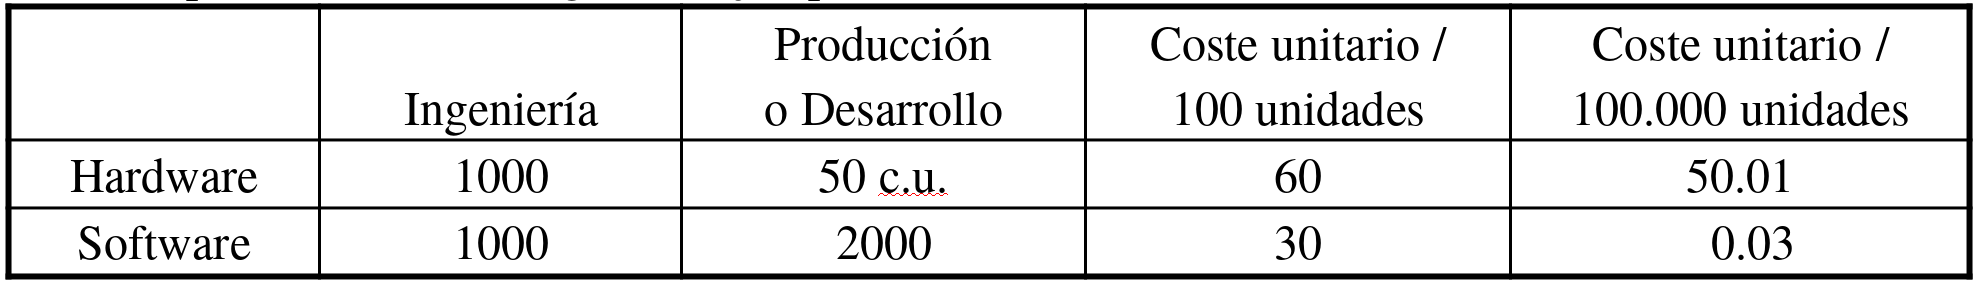
\includegraphics[width=0.8\textwidth]{Resources/Tema1/CostesProduccion.png}
            \caption{Influencia de los costes de ingeniería en el coste total del producto.}
        \end{figure}
          
    \item \textbf{Curva de fallos con respecto al tiempo diferente}:
          El software no se estropea con el tiempo; sin embargo es común aplicar ciertos cambios al mismo durante su ciclo de vida debidos al mantenimiento. Por ello, es probable que se introduzcan nuevos errores, que se acumulan con el tiempo, degradando la calidad. \textbf{El software no se estropea, pero se deteriora}.
          \begin{figure}[h]
            \centering
            \includegraphics[width=0.4\textwidth]{Resources/fallosSoftwareReales.png}
            \includegraphics[width=0.4\textwidth]{Resources/fallosHardware.png}
            \caption{Curva de fallos del Software (Izquierda) y del Hardware (Derecha). Obsérvese como en el caso del software el índice de fallos se va acumulando. Idealmente, el software solo presentaría fallos al principio de su vida por errores no detectados durante el desarrollo.}
        \end{figure}
    \item \textbf{Baja reutilización de las partes}:
          Por lo general el software se construye a medida como un conjunto, provocando que la reutilización sea baja; consecuentemente, se perjudica el desarrollo del software. Existe una tendencia al alza en la reutilización de artefactos (no tienen por qué ser código) gracias a:
          \begin{itemize}
              \item La elaboración de librerías y frameworks.
              \item Aplicación de técnicas de programación estructurada, modular y orientada a objetos.
              \item Aplicación de patrones de diseño, que supone el poder reutilizar diseños, el lugar de solo código.
          \end{itemize}
          Una empresa debería identificar los artefactos reutilizables con los que cuente, para que sus empleados los utilicen.
\end{enumerate}

\section{Atributos deseables en el software}
Todo software debería contar con las siguientes características:
\begin{itemize}
    \item \textbf{Mantenibilidad}: Facilidad para realizar cambios.
    \item \textbf{Confiabilidad}: Capacidad para seguir funcionando de manera segura y correcta.
    \item \textbf{Eficiencia}: Utilización de la mínima cantidad necesaria de recursos.
    \item \textbf{Usabilidad}: Facilidad con la que las personas utilizan el software.
\end{itemize}

\subsection{Aplicaciones del software}
Es difícil clasificarlas y carece de mucho valor hacerlo. \textit{Pressman} lo hace de la siguiente forma:
\begin{itemize}
    \item \textbf{Software de sistemas}: Sirven a otros programas.
    \item \textbf{Software de aplicación}: Programas independientes que resuelven una necesidad específica.
    \item \textbf{Software científico y de ingeniería}: ``Devoradores de números''.
    \item \textbf{Software empotrado}: Reside en una memoria de sólo lectura de pequeños chips, y con funciones limitadas y muy específicas.
    \item \textbf{Software de línea de productos}: \textit{Middleware}; cuentan con una capacidad específica que muchos clientes pueden usar (procesador de textos, por ejemplo).
    \item \textbf{Aplicaciones web}.
    \item \textbf{Inteligencia artificial}: \textit{Redes neuronales} (máquinas de estados \textbf{NO}).
\end{itemize}
El objetivo de todo software es desempeñar una determinada función cumpliendo una serie de requisitos.

\section{Software heredado}
Se trata de software \textbf{desarrollado hace décadas} %CORBA 
que además \textbf{ha ido sufriendo cambios} a lo largo del tiempo para adaptarse a los requisitos cambiantes del negocio. Estos dos factores hacen que sea muy difícil, y por lo tanto caro, de tratar, \uline{y usualmente es crítico para los negocios} (COBOL). Como es de esperar, probablemente se sustente sobre procesos de desarrollo desfasados, y malas prácticas (falta de documentación, por ejemplo). \textit{Pressman} aconseja tocarlo lo mínimo posible, al menos mientras no sea necesario.

\section{Principales problemas asociados a la producción del software}
Muchos expertos argumentan que la crisis del software nunca se ha solucionado, y es que esta ingeniería arrastra desde hace tiempo los siguientes \textbf{problemas crónicos}, causados por las propias características del software y por los errores de quiénes intervienen en su producción:
\begin{enumerate}
    \item \textbf{Imprecisión en la planificación, y estimación de costes temporales y monetarios}: Es frecuente que surjan imprevistos al abordar proyectos de cierta complejidad, dando lugar a desviaciones. Además, sin una planificación detallada, es imposible hacer una estimación de costes e identificar las tareas conflictivas. Entre las causas podemos citar la falta de recogida de datos de proyectos anteriores (no acumular experiencia), y la tradicional falta de experiencia de los gestores de proyecto (gente que no tiene ni idea de software gestionando proyectos o viceversa).
    \item \textbf{Baja productividad}: Los proyectos de software tienen a una duración mayor a lo esperada y, por lo tanto, mayores costes, y menor productividad y beneficios. Entre los múltiples motivos, se encuentran las especificaciones ambiguas o incorrectas, la poca comunicación con el cliente hasta la entrega, con sus consecuentes cambios de última hora, y la falta de documentación. Este problema culmina con que sea más costoso realizar una modificación sobre un programa que el rehacerlo.
    \item \textbf{Mala calidad}: El que las especificaciones sean ambiguas o incorrectas, junto con falta de realización de pruebas exahustivas, propicia la entrega de software con muchos errores, y por lo tanto incrementa los costes durnte el mantenimiento.
    \item \textbf{Insatisfacción del cliente}: Debida a los problemas anteriores, los clientes suelen quedar poco satisfechos con los resultados.
\end{enumerate}
\newpage
\part{El proceso}

\section{Conceptos}

\paragraph{Ingeniería del Software} Aplicación de un enfoque sistemático, disciplinado y cuantificable hacia el desarrollo, operación y mantenimiento del software; es decir, la aplicación de la ingeniería al software (IEEE).\\

Es necesaria para \uline{identificar y conocer las causas de los problemas en el desarrollo del software}, combinando las metodologías necesarias, dado que no van a desaparecer de la noche a la mañana. Está implícita la existencia de fases, de modo que la ingeniería del software proporciona una metodología que indica en cada momento los pasos a seguir, así como permite identificar en qué parte del proceso de ingeniería estamos y cuán bien lo estamos haciendo.

\paragraph{Tarea} Cualquier acción que transforma una entrada en salidas; el objetivo debe de ser pequeño y bien definido. \textit{Por ejemplo: ejecución del caso de prueba}.


\paragraph{Actividad} Conjunto de tareas que producen un producto importante del trabajo. \textit{Por ejemplo: desarrollo de un plan de pruebas.}

\paragraph{Proceso} Conjunto de actividades, y tareas que se ejecutan para llevar a cabo algún producto de trabajo. Este conjunto es \textbf{adaptable} a las necesidades del que lo utiliza. \textit{Por ejemplo: Validación}.

\paragraph{Modelo de los procesos} Descripción de los procesos involucrados en el desarrollo del software sin especificar cómo se desarrollan: \textit{Por ejemplo: IEEE 1074, ISO 12207-1 e ISO/IEC TR 15504-2}.

\paragraph{Métodos y procedimientos} Determinan el modo en el que se \textit{ejecutan las tareas}, determinando qué técnicas se utilizan en cada fase y cómo. \textit{Por ejemplo: IEEE 1008}.

\paragraph{Técnica} Cualquier recurso utilizado para llevar a cabo una tarea. Normalmente se habla de gráficos con apoyos textuales. \textit{Por ejemplo: Cobertura de caminos}.

\paragraph{Herramienta} Cualquier software que ayude en cualquier etapa del desarrollo. \textit{Por ejemplo: JUnit}.


\section{Procesos para la construcción del software}


La construcción del software incluye una serie de actividades que se empiezan a estandarizar. \textit{Pressman} la divide en \textbf{3 fases}:

\begin{enumerate}
    \item \textbf{Fase de definición}: Se centra en el \textbf{qué}, intentando identificar la información a procesar, la función y rendimiento esperados, las restricciones de diseño, las interfaces a utilizarse, los sistemas operativos y de hardware a utilizar, y los criterios de validación. Se identifican 3 actividades:
    \begin{itemize}
        \item \textbf{Análisis del sistema}: Define el papel de cada elemento relacionado con el sistema informático a desarrollar.
        \item \textbf{Análisis de requisitos del software}: Proporciona el ámbito del software y su relación con el resto de componentes del sistema.
        \item \textbf{Planificación}: Organización de las tareas que se llevarán a cabo en el proyecto.
    \end{itemize}
    El análisis y definición de requisitos es una tarea que debe ser llevada a cabo conjuntamente por el desarrollador de software y el cliente. \uline{Esta etapa produce el documento de especificación de requisitos del software.}
    \item \textbf{Desarrollo}: Se intenta definir \textbf{cómo} han de diseñarse las estructuras de datos, cómo ha de implementarse la función dentro de una arquitectura software, cómo han de implementarse los detalles procedimentales, cómo han de caracterizarse las interfaces, cómo ha de traducirse el diseño en un lenguaje de programación y cómo han de realizarse la pruebas. Se definen 3 actividades: 
    \begin{itemize}
        \item \textbf{Diseño del software}.
        \item \textbf{Codificación}.
        \item \textbf{Pruebas}.
    \end{itemize}
    \item \textbf{Mantenimiento}: Se centra en el cambio asociado a la corrección de errores, a las adaptaciones requeridas a medida que evoluciona el entorno del software, y a los cambios debidos a las mejoras producidas por los requisitos cambiantes del cliente. Se definen 4 actividades:
    \begin{itemize}
        \item \textbf{Adaptación} (cambio del entorno).
        \item \textbf{Corrección} (errores).
        \item \textbf{Mejora} (cambios en los requisitos).
        \item \textbf{Prevención} (mejor ingeniería).
    \end{itemize}
\end{enumerate}

\textbf{Nota:} \textit{Estas actividades se aplican de forma iterativa según la última versión de Pressman. Por ejemplo, un proceso de mantenimiento, como puede ser la corrección de un error grande, encajaría como una iteración de este modelo y no como una actividad concreta.}

\subsection{Norma IEEE 1074 -- 2006}
Proporciona el conjunto de actividades que constituyen los procesos que son necesarios para el correcto desarrollo y mantenimiento del software. Los procesos se dividen en 4 secciones lógicas:

\begin{enumerate}
    \item \textbf{Modelo del Ciclo de Vida Software}. Actividades para seleccionar el modelo de ciclo que \textbf{mejor se adapte} al proyecto; es necesario escoger uno. Además, \uline{la versión de 2006 requiere que se evalúe el riesgo}.
    \item \textbf{Grupos de Actividades de Gestión del Proyecto}. Son los procesos que inician, supervisan y controlan los proyectos de software a lo largo de su ciclo de vida.
          \begin{itemize}
              \item \textbf{Iniciación del proyecto}: Se crea el ciclo de vida y se definen las métricas para la gestión del proyecto.
              \item \textbf{Planificación y control del proyecto}: Se desarrollan planes para la evaluación, gestión de la configuración, instalación, integración, etc.
              \item \textbf{Monitorización y control}: Actividades de gestión de riesgos, gestión de proyecto, mejoras del ciclo de vida, recolección y análisis de métricas, y cierre del proyecto.
          \end{itemize}
    \item \textbf{Grupos de Actividades Orientadas al desarrollo}. Comprenden los procesos que se realizan antes, durante y después del desarrollo software.
          \begin{itemize}
              \item Pre--desarrollo:
                    \begin{itemize}
                        \item Análisis de la necesidad del sistema.
                        \item Asignación de requisitos del sistema al software y al hardware (solo si se trabajará con ambos).
                    \end{itemize}
              \item Desarrollo:
                    \begin{itemize}
                        \item Análisis de requisitos.
                        \item Diseño de arquitectura, BBDD, interfaces\ldots
                        \item Implementación (codificación, documentación, integración, gestión de versiones\ldots).
                    \end{itemize}
              \item Post--desarrollo:
                    \begin{itemize}
                        \item Instalación.
                        \item Operación y Soporte.
                        \item Mantenimiento.
                        \item Retirada.
                    \end{itemize}
          \end{itemize}
    \item \textbf{Grupos de Actividades de Soporte}: Necesarios para asegurar terminación y \textbf{calidad de los procesos} y, por lo tanto, del proyecto.
          \begin{itemize}
              \item Verificación y Validación (aseguramiento de la calidad).
              \item Gestión de Configuración Software.
              \item Desarrollo de documentación.
              \item Formación.
          \end{itemize}
\end{enumerate}

\subsection{Norma ISO 12207--1}
Define una serie de actividades que se realizan en la construcción del software, agrupadas en \textbf{cinco procesos principales, ocho de soporte, y cuatro de la organización}. \uline{No fomenta ningún modelo concreto de ciclo de vida, gestión del software o método de ingeniería}, ni prescribe cómo realizar las actividades o cómo organizarlas, aunque sí realiza una distinción entre el sistema y el software que se realiza para este.

\subsubsection{Procesos principales}
Los procesos principales resultan \uline{útiles a las personas que inician o realizan el desarrollo, la explotación o el mantenimiento del software durante su ciclo de vida}. Consisten en:
\begin{enumerate}
    \item \textbf{Proceso de adquisición}: Contiene las actividades realizadas por el cliente para adquirir un software. \textit{Ej: Solicitud de ofertas, o selección del suministrador}.
    \item \textbf{Proceso de suministro}: Contiene las actividades que realiza el suministrador. Incluye la preparación de la oferta para responder a una solicitud, y la identificación de los recursos y procedimientos para garantizar el éxito del proyecto.
    \item\textbf{Proceso de desarrollo}: Contiene numerosas actividades:
    \begin{itemize}
        \item \uline{Análisis de requisitos del sistema}: Funcionales y no funcionales.
        \item \uline{Diseño de la arquitectura del sistema}: Principales componentes de hardware y software.
        \item \uline{Análisis de los requisitos del software}: Se definen y documentan (pruebas de aceptación).
        \item \uline{Diseño de la arquitectura del software}: Se transforman los requisitos en una estructura de alto nivel en la que se pueden identificar los componentes principales. Se elabora una versión previa de los manuales, se define qué deben cumplir las pruebas de estos componentes, y se planifica la integración.
        \item \uline{Diseño detallado del software}: Se diseña de forma detallada cada componente de software. Se actualizan los manuales, se define qué deben cumplir las pruebas de estos componentes, y se planifican las pruebas unitarias.
        \item \uline{Codificación y prueba}: Se desarrollan y documentan los componentes software, y se prueba cada uno. Se actualizan los manuales.
        \item \uline{Integración del software}: Se integran los componentes del software y se prueban según sea necesario. Se actualizan los manuales.
        \item \uline{Prueba del software}: En función de los requisitos especificados para él.
        \item \uline{Integración del sistema}: Integración de elementos software y hardware.
        \item \uline{Prueba del sistema}: De acuerdo con los requisitos de cualificación especificados para el sistema.
        \item \uline{Instalación}: En el entorno de explotación final.
        \item \uline{Soporte del proceso de aceptación}: Apoyo a la revisión de aceptación y prueba por parte del comprador.
    \end{itemize}
    \item \textbf{Proceso de explotación}: Contiene la explotación del software y el soporte operativo a los usuarios.
    \item \textbf{Proceso de mantenimiento}: Modificación del código o documentación del software, como consecuencia de errores o deficiencias, mejoras, adaptaciones, y migraciones o retiradas del sistema.
\end{enumerate}

\subsubsection{Procesos de soporte}
Sirven de apoyo al resto y se aplican en cualquier punto del ciclo de vida.
\begin{enumerate}
    \item \textbf{Proceso de documentación}: Registra la información producida por cualquier proceso o actividad del ciclo de vida.
    \item \textbf{Proceso de gestión de la configuración}: Procesos administrativos para contar una línea base de los elementos configurables del software, hacer el control de cambio sobre estos elementos, registrar su estado y peticiones de cambio, asegurar su consistencia y corrección si es necesaria, y controlar su almacenamiento y distribución.
    \item \textbf{Proceso de aseguramiento de la calidad}: Asegurar que los procesos y productos cumplen con los requisitos especificados y se ajustan a los planes establecidos.
    \item \textbf{Proceso de verificación}: Determina si los requisitos de un sistema o del software están completos y son correctos, y si los \textbf{productos software de cada fase} del ciclo de vida cumplen los requisitos o condiciones impuestos en fases previas.
    \item \textbf{Proceso de validación}: Sirve para determinar si el \textbf{sistema o software final} cumple con los requisitos previstos para su uso.
    \item \textbf{Proceso de revisión conjunta}: Evaluación del estado del software y sus productos en su conjunto.
    \item \textbf{Proceso de auditoría}: Permite determinar, mediante hitos predeterminados, si se han cumplido los requisitos, los planes y el contrato.
    \item \textbf{Proceso de resolución de problemas}: Analiza y elimina los problemas descubiertos durante el desarrollo, la explotación, el mantenimiento u otro proceso.
\end{enumerate}

\subsubsection{Procesos de la organización}
Ayudan a conseguir que la organización sea más efectiva. Se llevan a cabo fuera del ámbito de proyectos y contratos específicos.

\begin{enumerate}
    \item \textbf{Proceso de gestión}: Planificación, seguimiento y control, evaluación, etc.; es decir, actividades genéricas para la gestión de procesos.
    \item \textbf{Proceso de infraestructura}: Dota a los demás procesos de la infraestructura necesaria, incluyendo hardware, software, normas, herramientas\ldots
    \item \textbf{Proceso de mejora}: Referente a los procesos del ciclo de vida.
    \item \textbf{Proceso de formación}: Mantener al personal formado.
\end{enumerate}

\subsection{Norma ISO/IEC TR 15504--2 (2003)}
Se puede considerar una ampliación a la norma ISO 12207 – 1 ya que \uline{amplía o añade procesos}. Además de ello, también expresa la capacidad que una empresa ha logrado en el desarrollo de un proceso. Los procesos que se añaden son los siguientes:

\begin{itemize}
    \item Procesos Principales: \textbf{Obtención de requisitos} (necesidades y requisitos del cliente).
    \item Procesos de Organización: \textbf{Gestión de recursos humanos} (proporcionar a la organización y proyectos los individuos con las habilidades y conocimiento efectivos), \textbf{alineamiento de la organización} (visión, cultura y compresión de los objectivos común), \textbf{medida} (recogida y análisis de datos relativos a los productos desarrollados) y \textbf{reutilización}. \textbf{El proceso de gestión, de los procesos de la organización, se divide} ahora en:
          \begin{itemize}
              \item Gestión \textbf{general}: Iniciación y realización de cualquier proceso.
              \item Gestión del \textbf{proyecto}: Asegurar que un proyecto produzca el resultado esperado, cumpliendo con los requisitos.
              \item Gestión de \textbf{calidad}: Con el objetivo de satisfacer al cliente.
              \item Gestión de \textbf{riesgos}: Identificar y reducir continuamente riesgos en un proyecto a lo largo de su ciclo de vida.
          \end{itemize}
\end{itemize}


\subsection{Norma ISO 12207 (2008)}

Esta actualización hace un \uline{mayor énfasis en la distinción entre el sistema y el software} realizado para este, al agrupar los procesos en dos categorías, los \textit{System Context Processes} y los \textit{Software Context Processes}.

\textbf{Descripción de procesos en la Norma ISO 12207 (2008):}

\begin{enumerate}
    \item \textbf{Identificador}: Categoría y número secuencial.
    \item \textbf{Título}.
    \item \textbf{Propósito}.
    \item \textbf{Resultados observables}.
    \item \textbf{Actividades y tareas}.
\end{enumerate}


\section{Evaluación del proceso software}
Como respuesta a los problemas generados por desarrollar software sin seguir un proceso o una metodología orientados a la calidad, las empresas se interesaron en encontrar y seguir procesos que les garantizasen los resultados. Sin embargo, en muchos casos se aplicaban de forma incompleta e inconsistente. De ello, surge una serie de métodos de evaluación y mejora de los procesos de la ingeniería del software.
\\\\
Objetivos:
\begin{itemize}
    \item \uline{De cara al contratante} de la empresa de software, proporcionar una medida de \textbf{cuán confiable} es que la empresa ofrezca sus servicios de creación y mantenimiento de software en tiempo y forma.
    \item \uline{De cara a la desarrolladora}, pretenden guiarla en la \textbf{mejora continua de sus procesos} de ingeniería.
\end{itemize}

\begin{figure}[H]
    \centering
    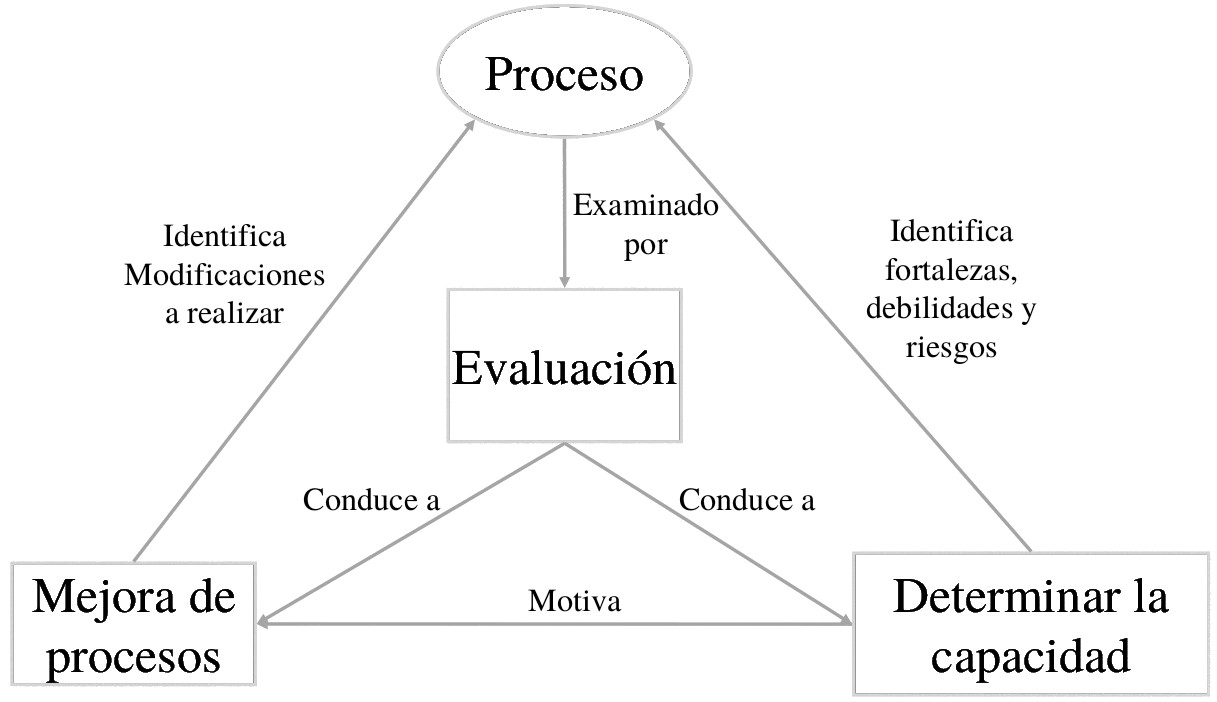
\includegraphics[width=0.6\linewidth]{Resources/evaluacionSoftware}
    \caption{Esquema de la evaluación del proceso software.}
    \label{fig:evaluacionSoftware}
\end{figure}

\subsection{Capability Maturity Model Integration (CMMI)}

Es un modelo que centra su evaluación en un total de 22 \textbf{áreas del proceso} categorizadas en:

\begin{itemize}
    \item Gestión de procesos.
    \item Gestión de proyectos.
    \item Ingeniería.
    \item Soporte.
\end{itemize}

Existen dos versiones del modelo:

\paragraph{Modelo continuo} Define el nivel de \uline{capacidad de cada una de las áreas del proceso} (es decir, de manera independiente entre ellas), mediante \textbf{metas genéricas} y \textbf{prácticas genéricas} que se aplican a cada área/proceso (las prácticas convierten una meta en un conjunto de actividades). Cada meta se corresponde a su vez con un nivel de capacidad. Por lo tanto, para alcanzar un nivel de capacidad particular en un proceso determinado, se debe alcanzar su meta genérica en él.\\

Los niveles de capacidad para un proceso son:

\begin{enumerate}
    \setcounter{enumi}{-1}
    \item \textbf{Incompleto}: El área del proceso aún no se realiza, o todavía no alcanza todas las metas para el nivel 1 de capacidad.
    \item \textbf{Realizado}: Todas las metas específicas del área han sido satisfechas.
    \item \textbf{Gestionado}: Además, el trabajo del área se ajusta a una política organizacional definida (control, revisión y evaluación), y se implica al cliente cuando sea necesario.
    \item \textbf{Definido}: Además, el proceso contribuye al proceso organizacional.
    \item \textbf{Cuantitativamente gestionado}: Además, el área se controla y mejora mediante mediciones cuantitativas.
    \item \textbf{En optimización (o en proceso de mejora)}: Ademas, el área se adapta y mejora mediante medios cuantitativas a las necesidades cambiantes del cliente.
\end{enumerate}

Adicionalmente, cada área del proceso tiene un conjunto de \textbf{metas específicas} a alcanzar en ella, así como las \textbf{prácticas específicas} requeridas para ellas.\\

Mediante el establecimiento de metas, se pretende definir las características que deben existir para que las actividades del área del proceso sean efectivas. 

\paragraph{Modelo discreto} Permite establecer el nivel de \uline{madurez global de los proyectos y de la organización}. Mientras que define las mismas áreas y metas específicas para cada proceso, la principal diferencia entre las dos versiones es que el modelo discreto solo define las metas generales 2 y 3 tal y como se habían descrito, junto con cinco niveles de madurez, en vez de cinco niveles de capacidad (\textit{un nivel de madurez es para un conjunto de áreas, mientras que un nivel de capacidad es para cada área, tal y como se muestra a continuación}):

\begin{enumerate}
    \item Nivel por defecto.
    \item Se deben cumplir las metas generales 2 para cada para siete áreas del proceso.
    \item Se deben cumplir las metas generales 2 y 3 para 18 áreas del proceso.
    \item Solo añade 2 áreas del proceso, que deben cumplir las metas generales 2 y 3.
    \item Solo añade 2 áreas del proceso, que deben cumplir las metas generales 2 y 3.
\end{enumerate}

\textbf{Nota:} \textit{La diferencia entre las dos versiones es meramente organizacional, y los contenidos son equivalentes.}

\paragraph{Standard CMMI Appraisal Method for Process Improvement (SCAMPI)}

Método oficial mediante el cual realizar análisis de calidad en CMMI, con el objetivo de identificar los puntos fuertes y débiles de procesos, revelar riesgos, y determinar los niveles de capacidad y madurez.\\

\newpage
\part{Ciclos de vida}

\paragraph{Ciclo de vida}  Sucesión de etapas por las que pasa el software desde que se concibe hasta que se deja de utilizar.

\paragraph{Etapa del ciclo} Lleva asociada una serie de tareas y de documentos \textit{(en sentido amplio: software)} de \textbf{salida} que serán la \textbf{entrada} de la fase siguiente.

\paragraph{Elección de un ciclo de vida} Se realiza de acuerdo con la naturaleza del proyecto, los métodos a usar, y los controles y entregas requeridos.

\section{Ciclo de vida en cascada}
\begin{figure}[H]
   \centering
   \includegraphics[width=0.7\linewidth]{Resources/cicloCascada}
   \caption{Etapas del ciclo de vida en cascada.}
   \label{fig:procesoCascada}
\end{figure}
El ciclo de vida en cascada es el más antiguo, surgido directamente de la copia del ciclo convencional de una ingeniería. Exige un enfoque sistemático y \textbf{secuencial} del desarrollo de software. Se dice que el modelo en cascada está guiado por documentos, ya que \textbf{nunca empieza la siguiente fase antes de que presente el documento de la anterior} (Tabla \ref{tab:cascadaDocumentos}).\\

\begin{table}[H]
   \centering
   \resizebox{\textwidth}{!}{%
      \begin{tabular}{|l|l|}
         \hline
         \multicolumn{1}{|c|}{\textbf{Proceso}} & \multicolumn{1}{c|}{\textbf{Documentos Producidos}}        \\ \hline
         Especificaciones del sistema.          & Especificación funcional. Arquitectura del sistema         \\ \hline
         Análisis de requisitos                 & Documento de requisitos                                    \\ \hline
         Diseño de la arquitectura del software & Especificación de la arquitectura                          \\ \hline
         Diseño de interfaces                   & Especificación del diseño                                  \\ \hline
         Codificación                           & Código de programa                                         \\ \hline
         Prueba de unidades                     & Informe de pruebas de unidad                               \\ \hline
         Prueba de módulos                      & Informe de pruebas de módulo                               \\ \hline
         Prueba de integración                  & Informe de prueba de integración y manual de usuario final \\ \hline
         Prueba del sistema                     & Informe de prueba del sistema                              \\ \hline
         Prueba de aceptación                   & Sistema final más la documentación                         \\ \hline
      \end{tabular}%
   }
   \caption{Ejemplo de documentos producidos en un ciclo de vida en cascada. \textit{No tiene que tener exactamente las mismas fases que el ciclo en cascada por defecto.}}
   \label{tab:cascadaDocumentos}
\end{table}

\subsection{Fases}
\begin{enumerate}

   \item \textbf{Ingeniería y análisis del sistema}: Define las interrelaciones del software con otros elementos del sistema más complejo en el que esté englobado; es decir, se asignan funciones del sistema al software. Por tanto, comprende los requisitos globales a nivel de sistema, mediante un análisis y diseño a alto nivel.

   \item \textbf{Análisis de requisitos del software}: Análisis detallado de los componentes del sistema implementados mediante software incluyendo \textbf{datos} a manejar, \textbf{funciones} a desarrollar, \textbf{interfaces}, y \textbf{rendimiento} esperado.
   
   \textbf{Nota:} \textit{Los requisitos, tanto del sistema como del software, deben documentarse y revisarse con el cliente.}

   \item \textbf{Diseño}: En cuanto a estructura de los datos, arquitectura de las aplicaciones, estructura interna de los programas, y las interfaces. Es un proceso que traduce los requisitos en una representación del software que permita conocer la arquitectura, funcionalidad e incluso la calidad antes de codificar.

   \item \textbf{Codificación}: Traducción del diseño a un formato que sea legible para la máquina.
   
   \textbf{Nota:} \textit{Como se puede observar, estas primeras fases del ciclo de vida consisten básicamente en una traducción de documentos.}

   \item \textbf{Prueba}: Verificar que no se hayan producido errores en alguna de las fases de traducción anteriores. Deben probarse todas las sentencias de todos los módulos, y no solo los casos ``normales''.

   \item \textbf{Utilización}: Entrega del software al cliente y comienzo de su vida útil. Es una etapa que se solapa con las posteriores.
   
   \item \textbf{Mantenimiento}: El software sufrirá cambios a lo largo de su vida útil debido a que el cliente detecte errores, que se produzcan cambios en alguno de los componentes del sistema, o que el cliente requiera modificaciones funcionales. Estos cambios requieren volver atrás en el ciclo de vida (etapas de codificación, diseño o incluso análisis), en función de la magnitud del cambio.
   
   \textbf{Nota:} \textit{El modelo en cascada, a pesar de ser lineal, contiene flujos que permiten la vuelta atrás. Además del mantenimiento, se puede volver desde cualquier fase a la anerior si se detectan fallos. Estas vueltas atrás no son controladas y quedan reflejadas en el modelo.}

  \item \textbf{Sustitución}: Cualquier aplicación acaba siendo sistituida. Es una tarea que debe planificarse cuidadosamente y, si es posible por fases:
  
  \begin{enumerate}
      \item Trasvase de la información que maneja el sistema viejo al formato del nuevo.
      \item Mantención de los dos sistemas funcionando en paralelo para comprobar que el nuevo funciona correctamente.
      \item Sustitución completa del sistema antiguo.
  \end{enumerate}
\end{enumerate}

\subsection{Aportaciones}
\begin{itemize}
   \item Es el más simple, conocido y fácil de usar.
   \item Los procesos definidos se \textbf{formalizan} en normas, \textit{sabes lo que tienes que hacer en cada momento}.
   \item Permite generar software eficientemente, y de acuerdo a las especificaciones: no sobrepasar fechas de entrega ni costes esperados.
   \item Al final de cada fase, los interesados pueden comprobar el estado del proyecto.
\end{itemize}

\subsection{Problemas}
\begin{itemize}
   \item En realidad los \textbf{proyectos no siguen un ciclo de vida estrictamente secuencial}, sino que siempre hay iteraciones. Un claro ejemplo de ello es la fase de mantenimiento, aunque es frecuente detectar errores en cualquiera de las otras fases. 
   \item No siempre se pueden establecer los requisitos desde el primer momento, sino lo normal es que se vayan aclarando y refinando a lo largo de todo el proyecto. Es habitual que los clientes no tengan el conocimiento de la importancia de la fase de análisis, o bien no hayan pensado en detalle qué quieren del software.
   \item Hasta que se llega a la fase final, no se dispone de una versión operativa del programa. Esto no resulta óptimo, dado que la mayor parte de los fallos suelen detectarse una vez el cliente puede probar el programa; al final del proyecto, es cuando más costosos son de corregir, y cuando más prisas hay.
   \item Se producen estados de bloqueo, dado que una fase no puede comenzar sin los documentos de salida de la anterior.
\end{itemize}

\textbf{Nota:} \textit{A pesar de ello, es mucho mejor desarrollar software siguiendo el modelo de ciclo de vida en cascada, que hacerlo sin ningún tipo de guías.}


\section{Construcción de prototipos}

Este ciclo de vida palia directamente las deficiencias del ciclo de vida en cascada de que:

\begin{itemize}
   \item Sea difícil tener claros todos los requisitos al inicio del proyecto.
   \item No se disponga de una versión operativa del programa hasta las fases finales.
\end{itemize}

\subsection{Sistemas que resultan ser buenos candidatos}

\begin{itemize}
   \item Resulta idóneo en \textbf{proyectos con un nivel alto de incertidumbre}, donde los requisitos no están nada claros en primera instancia, ya que se provee un \textbf{método para obtener los requisitos de forma fiable} a través del feedback del usuario. Por lo tanto, debería omitirse ante problemas bien comprendidos.
   \item También es de especial interés en aplicaciones que presenten mucha interacción con el usuario, o algoritmos evolutivos.
   \item La aplicación no debe contar con una gran complejidad, o las ventajas de la construcción de prototipos se verán superadas por el esfuerzo de un prototipo que habrá que desechar o modiificar mucho.
   \item El cliente debe estar dispuesto a probar un prototipo.
\end{itemize}

%Foto de ciclo prototipos
\begin{figure}[H]
   \centering
   \includegraphics[width=0.7\linewidth]{Resources/construccionPrototipos.png}
   \caption{Etapas del paradigma de la construcción de prototipos.}
   \label{fig:construccionPrototipos}
\end{figure}

\subsection{Beneficios de los prototipos}

\begin{itemize}
   \item Permiten probar la eficiencia en condiciones similares a las que existirán durante la Utilización del sistema.
   \item Permiten mostrar al cliente la E/S de datos en la aplicación, para detectar problemas en la especificación.
   \item Gran parte del trabajo realizado puede ser utilizado en el diseño final. El diseño se paracerá cada vez más al del producto final, meintras que los componentes codificados deberán ser generalmente optimizados.
   \item Los prototipos permiten analizar \textbf{alternativas y viabilidades}, refinando el resultado final o abortándolo antes de invertir demasiado dinero en el mismo.
\end{itemize}

\subsection{Formas de prototipos}

\begin{itemize}
   \item En papel o ejecutable, que describa la interacción con el usuario.
   \item Que implemente subconjuntos de la funcionalidad requerida, para evaluar el rendimiento.
   \item Que realice todo o en parte, pero con características que todavía deban ser mejoradas.
\end{itemize}

\subsection{Construcción de un prototipo}

\begin{enumerate}
   \item Realizar un modelo del sistema a partir de los requisitos conocidos. No es necesario realizar una definición completa de estos.
   \item Diseñar rápidamente el prototipo, centtrándose en la arquitectura del sistema y en las interfaces, antes que en aspectos procedimentales.
   \item Construir el prototipo, mediante una codificación rápiday que facilite el desarrollo incremental. Es irrelevante la calidad obtenida.
   \item Presentar el prototipo al cliente para que lo pruebe y sugiera modificaciones.
   \item Con estos comentarios, proceder a construir un nuevo prototipo, y así sucesivamente, hasta que los requisitos queden completamente formalizados y se pueda comenzar a desarrollar el producto final.
\end{enumerate}

\textbf{Nota:} \textit{Como se puede comprobar, el prototipado es una técnica que sirve fundamentalmente para la fase de análisis de requisitos.}\\

\textbf{Nota:} \textit{El prototipo no es el sistema final.}

\subsection{Problemas}
\begin{itemize}
   \item En muchas ocasiones, el prototipo, que carece de calidad, pasa a ser parte del sistema final por presiones, o bien por que los técnicos se hayan acostumbrado a él.
   \item Es \textbf{posible que nunca se llegue a la fase de construcción} por falta de recursos, lo cual da lugar a los problemas característicos de un software construido sin seguir procesos de ingeniería al emplear el prototipo como sistema final.
   \item Es imposible una \textbf{predicción de costes} fiable.
\end{itemize}


\section{Ciclo de vida incremental}
% foto de incrementos
\begin{figure}[H]
   \centering
   \includegraphics[width=0.7\linewidth]{Resources/cicloIncremental.png}
   \caption{Etapas del ciclo de vida incremental.}
   \label{fig:procesoIncremental}
\end{figure}

Combina elementos del \textbf{modelo lineal} en cascada con la \textbf{filosofía iterativa} de construcción de prototipos. Para ello, se va creando el sistema software mediante incrementos, aportando nuevas funcionalidades o requisitos. De este modo el software ya no se ve como un producto con una fecha de entrega, sino como una \textbf{integración de sucesivos refinamientos}.\\

A diferencia del modelo por prototipos, el incremental se centra en obtener un producto operativo en cada iteración; los primeros incrementos simplemente son versiones incompletas del producto final.

\paragraph{Incrementos} Componentes funcionales del sistema. Cada incremento es una parte completa y funcional del sistema por sí misma.

\subsection{Sistemas que resultan ser buenos candidatos}

\begin{itemize}
   \item Entornos con incerditumbre.
\end{itemize}

\textbf{Nota:} \textit{Nótese que se adapta bien a entornos de incertidumbre, mientras que el modelo basado en prototipos es más propio de entornos de \uline{alta} incertidumbre.}

\subsection{Ventajas}

\begin{itemize}
   \item Soluciona parte de los problemas del modelo en cascada, al mejorar la \textbf{comunicación con el cliente}, y al existir \textbf{detecciones de errores} con más atelación.
   \item Favorece la modulación del software al ser un modelo iterativo.
\end{itemize}

\subsection{Desventajas}

\begin{itemize}
   \item Dado que la parte de requisitos no se encuentra en la fase iterativa, es difícil ver si estos son válidos, y se siguen detectando relativamente tarde, al haberse construido ya productos operativos en cada iteración (mismos problemas que con el ciclo en cascada).
\end{itemize}


\section{Técnicas de cuarta generación}

Son un conjunto diverso de métodos y herramientas con el objetivo de facilitar el desarrollo de software, al permitir especificar características del software a alto nivel, y generar código fiente automáticamente a partir de estas especificaciones:

\begin{itemize}
   \item Acceso a bases de datos utilizando lenguajes de consulta de alto nivel, sin ser necesario conocer la estructura de esta.
   \item Generación de código.
   \item Generación de pantallas y entornos gráficos.
   \item Generación de informes.
\end{itemize}

Con esta automatización, se reduce la duración de las fases del ciclo de vida clásico, especialmente de la codificación.\\

A pesar de ello, estas técnicas no han obtenido los resultados previstos cuando se comenzaron a desarrollar, con intenciones de eliminar la necesidad de la codificación manual y de incluso analistas. Por lo menos, consiguen eliminar las tareas más repetivivas y tediosas.

\subsection{Críticas más habituales}

\begin{itemize}
   \item No son más fáciles de utilizar que los lenguajes de tercera generación.
   \item El código fuente que producen es ineficiente.
   \item Solo son generalmente aplicables al software de gestión.
\end{itemize}


\section{Modelo en espiral}

\begin{figure}[H]
   \centering
   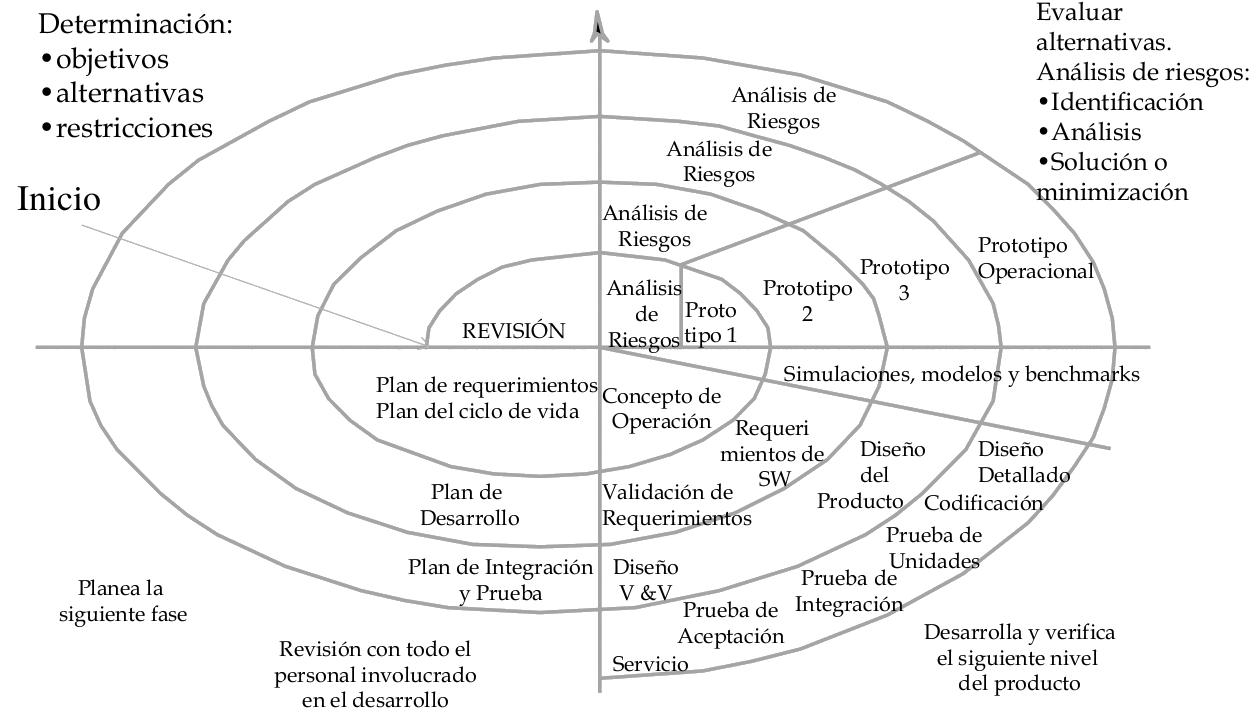
\includegraphics[width=0.9\linewidth]{Resources/Tema3/modeloEspiral.png}
   \caption{Etapas del modelo en espiral.}
   \label{fig:modeloEspiral}
\end{figure}

Es un \textbf{modelo iterativo que combina las principales ventajas del modelo de ciclo de vida en cascada y el modelo de construcción de prototipos}. Su principal característica es incorporar el \textbf{análisis de riesgos} en el propio ciclo de vida, de modo que los prototipos son usados para reducir el riesgo, incluso permitiendo finalizar el proyecto antes de embarcarse en el desarrollo final si no se considera viable.\\

\textbf{Nota:} \textit{Mientras que el modelo iterativo toma la filosofía \uline{iterativa} del desarrollo de prototipos, el modelo en espiral toma directamente las ventajas de realizar prototipos.}


\subsection{Descripción del modelo}

El proceso se representa como una espiral, en donde cada ciclo representa una fase del proceso, en función de lo que mejor se ajuste al proyecto; por ejemplo, el ciclo más interno puede relacionarse con la factibilidad, el siguiente con la definición de requistios, el siguiente, con el diseño, etc. Siempre se actúa en función a los riesgos que el proyecto presente, y por ello se incluyen las actividades de la gestión de riesgos para reducirlos.

Se definen un total de cuatro sectores:

\begin{enumerate}
   \item \textbf{Definición de objetivos}: Objetivos de la fase actual y restricciones con las que deben alcanzarse. Finaliza con la identificación de diferentes alternativas que permitirían alcanzar estos objetivos.
   \item \textbf{Análisis de riesgos}: Se identifican los riesgos de las diferentes alternativas, así como tratarlos, con el objetivo de escoger una de las alternativas.
   \item \textbf{Desarrollo y validación}: Se realiza el análisis de viabilidad de las alternativas y, si se ha reducido el riesgo a niveles aceptables, se realizan las actividades de ingeniería que construyen el producto; es decir, se general entregables de los procesos clásicos, siguiendo, por ejemplo, un ciclo en cascada.
   \item \textbf{Revisión y planificación}: \uline{Todas las personas implicadas}, incluso clientes, revisan los productos desarrolladores y se planificaría la ejecución del siguiente ciclo. Se finaliza con la toma de decisión de finalizar o continuar el proyecto.
\end{enumerate}


\subsection{Ventajas}

\begin{itemize}
   \item Es mucho más realista que el ciclo de vida clásico.
   \item Permite la utilización de prototipos en cualquier etapa de la evolución del proyecto.
   \item Existe un reconocimiento explícito de las alternativas para realizar un proyecto.
   \item Existe una identificación de los riesgos, junto con las diferentes maneras de tratarlos, eliminando las ilusiones de avance.
   \item Se adapta a cualquier tipo de actividad, incluso alejadas de un ciclo de vida tradicional, como la consulta a asesores externos.
\end{itemize}


\subsection{Desventajas}
\begin{itemize}
   \item El modelo en espiral se adapta bien a los desarrollos internos, pero necesita un ajuste para la contración de software, al no contar con la flexibilidad para ajustar el desarrollo etata por etapa (por ejemplo, aplazar decisiones, pararse en miniespirales para realizar secciones críticas con precaución, etc.).
   \item Requiere expertos en la evaluació de riesgos, para realizar evaluaciones apropiadas y no abocarse al desastre.
   \item Resulta difícil de controlar, y de convencer al cliente de que es manejable.
\end{itemize}

\textbf{Nota:} \textit{En todo caso, podría plantearse la realización de un contracto como una iteración del ciclo en espiral}.


\subsection{Análisis de riesgos}

\subsubsection{Definiciones}

\paragraph{Activos} Elementos de un sistema de información que soportan los objetivos de la organización (presentan un cierto valor). Por ejemplo: equipamiento, redes de comunicación, instalaciones, personas, etc.

\paragraph{Amenazas} Qué puede pasarles a los activos, perjudicándolos consecuentemente. Pueden ser de origen natural, del entorno de trabajo, por defectos en el producto, y causados por las personas de forma accidental o deliberada.

\paragraph{Contramedidas} Medidas de protección desplegadas para que las amenazas no causen tanto daño.

\paragraph{Riesgo} Estimación del grado de exposición a que una amenaza se materialice sobre uno o más activos, causando perjuicios a la organización.

\paragraph{Análisis de riesgos} Proceso para estimar la magnitud de los riesgos a los que está expuesta una organización.

\paragraph{Proceso de gestión de riesgos} Proceso destinado a modificar un riesgo, para reducir su impacto.

\begin{figure}[H]
   \centering
   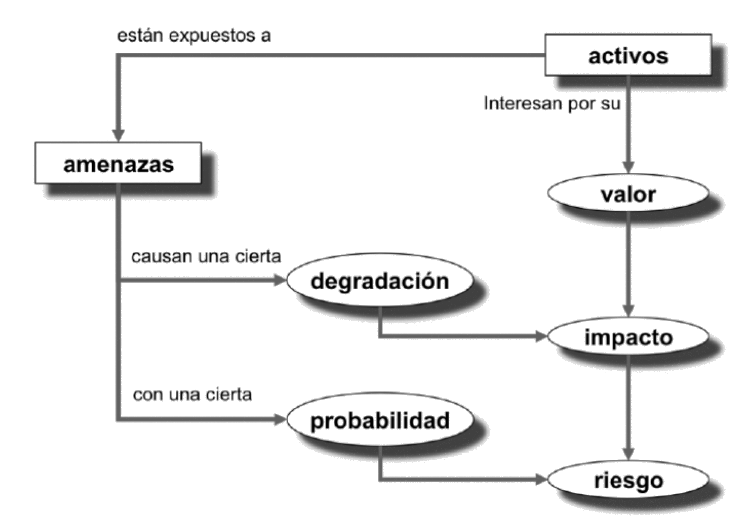
\includegraphics[width=0.6\linewidth]{Resources/Tema3/relacionesDefinicionesRiesgos.png}
   \caption{Elementos del análisis de riesgos potenciales.}
   \label{fig:relacionesDefinicionesRiesgos}
\end{figure}

\subsubsection{Anticipación a los riesgos}

Consta de cuatro actividades principales:

\begin{enumerate}
   \item \textbf{Identificar los riesgos} Se identifican los activos relevantes, a qué amenazas están expuestos, y los riesgos asociados. \textit{Sommerville} clasifica los riesgos en:
      
      \begin{itemize}
         \item Del negocio: Afectan a la organización (riesgos de mercado, mala reputación\ldots).
         \item Del proyecto: Afectan a la calendarización y los recursos.
         \item Del producto: Afectan a la calidad del producto.
      \end{itemize}

   \item \textbf{Análisis de riesgos}: Se evalua, empleando una escala a intervalos y según la experiencia de los expertos, la probabilidad de que cada riesgo ocurra (baja, moderada y alta, por ejemplo), así como sus consecuencias o impacto (catastrófico, grave, tolerable y e insignificante, por ejemplo). A pesar de emplear una escala a intervalos, cada uno de estos debe sustentarse sobre medidas objetivas; por ejemplo, un riesgo tolerable será aquel cuyo impacto no excede los márgenes temporales o económicos del proyecto. Esta actividad concluye con la elaboración de una lista ordenada de riesgos por importancia.

   \item \textbf{Planificación de riesgos}:
         Tras escoger aquellos riesgos más prioritarios, se establecen estrategias para gestionarlos, en base a la experiencia de nuevo:
         \begin{itemize}
            \item Estrategias de prevención.
            \item Estrategias de minimización.
            \item Planes de contingencia: estar preparados para lo peor.
            \item Transferencia: subcontratación de expertos que gestionen y \uline{se responsabilicen} de la gestión del riesgo.
         \end{itemize}
   \item \textbf{Gestión de riesgos}: Supervisar el desarrollo del proyecto continuamente, de forma que se detecten los riesgos tan pronto como aparezcan. Para ello, se definen indicadores cuatificables para cada riesgo, así como sus umbrales de alerta.
\end{enumerate}

\begin{figure}[H]
   \centering
   \includegraphics[width=0.7\linewidth]{Resources/administracionRiesgo.jpg}
   \caption{Administración del riesgos.}
   \label{fig:administracionRiesgo}
\end{figure}





\section{Metodologías ágiles}

Cabe destacar, en todo lo visto hasta el momento, el esfuerzo puesto en:

\begin{itemize}
   \item Documentar los proyectos.
   \item Buscar posibles fallos y seguir las correcciones y modificaciones que suponen, en lugar de centrarse en construir el software en sí.
   \item Garantizar la calidad del producto mediante un seguimiento riguroso de los procesos de construcción.
   \item Modificar los documentos resultantes, dado que no permanecen inmutables en el tiempo.
\end{itemize}

Como se puede ver, estas metodologías pesadas presentan una aproximación sistemática y disciplinada, con procesos fuertemente orientados a la documentación: la documentación no es un objetivo sino el medio para lograrlo y con calidad, y el formalismo da calidad a pesar de ralentizar el desarrollo.
%Sorprendente estos dos párrafos están bien.

El desarrollo ágil defiende la renuncia a utilizar estos modelos perfectos, se basa únicamente en que sean lo \uline{suficientemente buenos}. Tratan de \textbf{centrar los esfuerzos en presentar un incremento software ejecutable}, restando importancia a los productos de trabajo intermedio, que no siempre es bueno.\\

En el manifiesto para el desarrollo ágil, firmado por \textit{Kent Beck} entre otros, se establecía la valoración de:

\begin{itemize}
   \item Individuos e intenciones sobre los procesos.
   \item software en funcionamiento sobre la documentación.
   \item Colaboración con el cliente sobre el contrato.
   \item Respuesta al cambio sobre el seguimiento de un plan.
\end{itemize}

Como se puede ver, estos modelos resultan ser una corriente opuesta a la tradicional, no con el objetivo de eliminarlos, sino de solventar sus limitadas capacidades de adaptación al cambio, dada la fragilidad de los requisitos y la variabilidad del entorno, y la disciplina de trabajo exigida a las personas.\\

\subsection{Variabilidad del entorno}

Las metodologías ligeras proponen una aproximación incremental en donde se valora la entrega frecuente; por ejemplo, desarrollando incrementos tras un par de semanas o de meses. Estos son valorados por el cliente, entrando a ser partícipe del proceso de software, para que ofrezca el \textit{feedback} necesario, como nuevos requisitos o prioridades.

\subsection{Fragilidad por las debilidades humanas}

En contraposición a exigir una gran disciplina al personal para asegurar que los procesos se desarrollan correctamente, las metodologías ligeras aceptan tolerancia en la aplicación de los modelos, permitiendo que estos se adapten al equipo, y no al revés.\\

Algunos de los rasgos con los que las personas deberían contar son: competencia, enfoque común (entregar un incremento a tiempo), colaboración entre todos los \textit{stakeholders}, habilidades y técnicas para la toma de decisiones, capacidad de resolución de problemas ambigüos (debido al cambio), confianza y respeto mutuo, y organización propia para lograr los objetivos.

\subsection{Diferentes modelos de proceso}

\begin{itemize}
   \item Programación Extrema (PE).
   \item Desarrollo Adaptativo del Software (DAS).
   \item SCRUM.
   \item Cristal.
   \item Desarrollo conducido por características (DCC).
   \item Modelado Ágil.
\end{itemize}

\subsection{Modelado ágil}

A \textbf{alto nivel}, es una \textbf{colección de valores, pricipios y prácticas} (en resumen, buenas prácticas) que poder aplicar para realizar modelado y documentación de forma efectiva y ligera en un proyecto de desarrollo de software. Por ejemplo, es habitual la práctica de \textit{Test-Driven Development}, que consta a su vez de las dos prácticas de \textit{Test-First Development} y de refactorización.\\

Al final, el modelado ágil puede ser tomado más como una filosofía que como una metodología:

\begin{itemize}
   \item Modelar con un propósito: Trabajar siempre con un objetivo en mente.
   \item Conocer los modelos y notaciones disponibles, y usar el más apropiado para cada situación.
   \item Viajar ligero: Conservar sólo la documentación o modelos que proporcionarán valor a largo plazo, y que deberán recibir por lo tanto un mantenimiento.
   \item El contenido es más importante que la representación: Solo es necesario que un modelo pueda ser interpretado por la audiencia a la que está dirigido.
   \item Adaptar a las necesidades del equpo.
\end{itemize}

\subsection{Programación extrema}

\begin{figure}[H]
   \centering
   \includegraphics[width=0.7\linewidth]{Resources/programacionExtrema.jpg}
   \caption{Etapas de la programación extrema.}
   \label{fig:programacionExtrema}
\end{figure}

Utiliza, preferiblemente, un enfoque orientado a objetos, y abarca un conjunto de reglas y prácticas que ocurren las siguientes cuatro actiividades:

\begin{enumerate}

   \item \textbf{Planificación}:
         
      \begin{itemize}
            \item \textbf{Creación de historias de usuario}: Describen características y funcionalidades requeridas (permiten establecer requisitos); cada historia se asemeja a un caos de uso, es escrita por el cliente, y este le asigna una prioridad.
            \item \textbf{Estimación del tiempo de implementación}: Los miembros del equipo evalúan cada historia y asignan un coste en semanas de desrollo; si es superior a tres semanas, se segmenta la historia.\\
            \textbf{Nota:} \textit{Pueden escribirse historias en cualquier momento.}
            \item \textbf{Plan de construcción}: Los clientes y el equipo se reúnen para decidir qué historias hay en el siguiente incremento del software, priorizando siguiendo una de las siguientes vías:
                  \begin{itemize}
                     \item Todas las historias serán implementadas de un modo inmediato.
                     \item Las historias con \textbf{valor más alto} se implementarán al \textbf{principio}.
                     \item Las historias de \textbf{mayor riesgo} se implementarán al \textbf{principio}.
                  \end{itemize}
            \item \textbf{Cálculo de la velocidad del proyecto}: Tras cada lanzamiento, se recoge el número de historias implementadas, con la intención de:
                  \begin{itemize}
                     \item Ayudar a estimar futuras fechas de entrega y programaciones.
                     \item Determinar si, hasta el momento, ya se ha realizado algún compromiso no viable.
                  \end{itemize}
         \end{itemize}


   \item \textbf{Diseño}: Sigue el principio KISS (\textit{Keep It Simple, Stupid}), de modo que solo se implementa lo requerido, y se apoya en:
         % https://en.wikipedia.org/wiki/KISS_principle El stupid es importante. Porque somos estúpidos y debemos recordarlo.
         \begin{itemize} %Mejor así.
            \item \textbf{Tarjetas CRC} (Colaborador--Responsabilidad--Clase).
            \item \textbf{Soluciones de Pico}: Si se presenta un problema difícil, se recomienda construir un prototipo para probar dicha parte y analizarlo, de modo que se reduzca el riesgo a la hora de comenzar la verdadera implementación.
            \item \textbf{Refabricación} (\textit{Refactoring}): Cambiar un sistema de software de tal manera que no altere el comportamiento externo del código y que mejore la estructura interna (mejorar el diseño del código después de que haya sido escrito).
            \item \textbf{Diseño como artefacto}: Se permite la modificación del diseño durante todas las fases de la construcción.
         \end{itemize}

   \item \textbf{Codificación}:
   
   \begin{itemize}
      \item Después de realizar el trabajo de diseño preliminar, se prefiere crear las \textbf{pruebas de unidad que ejerciten cada una de las historias, antes que el código} de las clases. Así, el desarrollador se centra en implementar lo necesario para pasar la prueba de unidad y, una vez escrito el código, puede evaluarse de inmediato.
      \item Un concepto clave durante la codificación es la programación en pareja, con el objetivo de mejorar la capacidad de resolución de problemas y asegurar la calidad. En la práctica, cada persona tiene un papel sutilmente diferente.
      \item Una vez unos desarrolladores finalizan su trabajo, el código escrito debe integrarse con el trabajo de otros; mediante esta estrategia de integración continua, se evitan mayores problemas de compatibilidad e interfaz. Se realizan ``pruebas de humo'', que son pruebas de integración poco exhaustivas de todo el sistema con las que detectar los errores más importantes.
   \end{itemize}

   \item \textbf{Pruebas}:
         \begin{itemize}
            \item \textbf{Pruebas diarias}: Comprenderían, principalmente, las pruebas de unidad e integración, y deberían organizarse de forma que puedan ser automatizadas. Así, si se realizan a diario, se proporciona al equipo un indicador de progreso, así como una alarma fiable en caso de que las cosas vayan mal.
            \item \textbf{De aceptación o del cliente}: Estando especificadas por el cliente, se enfocan en las características generales y la funcionalidad del sistema, siempre sobre aspectos que el cliente pueda revisar. Se derivan de las historias de usuario implementadas.
         \end{itemize}
\end{enumerate}

\newpage
\part{Análisis de requisitos}

\section{Introducción}

En todos los modelos de ciclos de vida existe la fase de \textbf{análisis de requisitos}, en la cual se estudian las características y funciones del sistema, la definición de los requisitos del software y del sistema del que forma parte, la planificación inicial del proyecto, y tareas de análisis de riesgos. Este análisis se centra en la \uline{información, funcional y de comportamiento del problema}, el cual se divide en partes que se modelan para comprenderlo mejor, con el objetivo de desarrollar una \textbf{especificación de requisitos}, en donde se describe el problema analizado y la solución propuesta.\\

Como se puede prever, esta especificación se convierte en base de todas las actividades que siguen y, por ende, tiene una gran influencia en la calidad de la solución implementada finalmente. El principal problema es que, \uline{al inicio de un proyecto, es difícil tener una idea clara y segura de los requisitos del sistema y del software}, para comprender qué debe realizar este último; por ello, algunos de los ciclos de vida estudiados proponen enfoques cícliclos de refinamiento de los requisitos.

\subsection{Requisito}

Se define como una condición o capacidad que necesita el usuario para resolver un problema o conseguir un objetivo determinado. Por extensión, se corresponde también con las condiciones o capacidades que debe cumplir o poseer un sistema para satisfacer un contrato, una norma o una especificación.

\subsubsection{Características comunes a todos los requisitos}

\begin{itemize}
    \item Son una abstracción de las características del sistema (modelan el mismo).
    \item Representan el sistema de forma jerárquica, particionando el problema en varios niveles de detalle.
    \item Definen interfaces del sistema, tanto externas como internas.
    \item Sirven de base para las etapas posteriores del ciclo de vida.
    \item Existen requisitos de usuario, de sistema, esenciales, y de implementación.
    \item No prestan demasiada atención a las restricciones o criterios de validación (exceptuando los métodos de especificación formal).
\end{itemize}

\subsubsection{Clasificación de los requisitos}
\begin{itemize}
    \item \textbf{Requisitos funcionales}: Servicios que proveerá el sistema, concretando de qué manera reaccionará a entradas particulares, y cómo se comportará en situaciones particulares; también declaran lo que el sistema no debe hacer. \textit{Ejemplo: El usuario tendrá la posibilidad de buscar por tamaño}.
    
    Si un requisito funcional no se cumple, el sistema se verá degradado al no contener toda su funcionalidad.

    \item \textbf{Requisitos no funcionales}: Restricciones sobre los servicios o funciones ofrecidos por el sistema; es decir, no se refieren directamente a las funciones específicas del sistema, sino a propiedades de estas. Pueden ser temporales, de fiabilidad, de robustez, de capacidad, de ajuste a estándares, etc.; además, deben expresarse de forma cuantitativa. \textit{Ejemplo: La duración de la sesión ha de ser superior a 30 minutos}.
    
    Con frecuencia hacen referencia al sistema como un todo, por lo que los fallos en ellos lo inutilizan.

    \item \textbf{Requisitos del dominio}: Provienen del entorno en el que se realiza la aplicación, reflejando por lo tanto las características de este, y pueden ser funcionales o no funcionales. Dada esta naturaleza, presentan la dificultad de que sean expresados en un lenguage específico de la aplicación en donde el analista no comprenda todos los detalles. \textit{Ejemplo: usar el formato DICOM en medicina es a la vez un requisito no funcional y de entorno}.
    
    Es importante respetarlos dado que es imposible que el sistema trabaje satisfactoriamente si se incumplen.
\end{itemize}

\textbf{Nota:} \textit{Al expresar requisitos funcionales, es necesario ser precavido si se emplea el lenguaje natural, dado que puede dar lugar fácilmente a ambigüedades e inconsistencias.}

\subsection{Análisis de requisitos}

De forma concisa, y visto todo lo anterior, se podría decir que es el proceso de \textbf{estudio de las necesidades de los usuarios} para llegar a una definición de los requisitos obtenidos, incluyendo el proceso de refinamiento de los mismos.
\\\\
Cabe destacar que, dadas todas las dificultades que puede presentar, y presentará con alta probabilidad, es una fase que tiende a extenderse indefinidamente. El tiempo que se le dedique dependerá al final del propio proyecto, pero puede emplearse la regla de 40--20--40 como una guía; \textit{por norma general, se debería dedicar un 40\% del tiempo de desarrollo de un proyecto al análisis y diseño, un 20\% a la codificación, y un 40\% a la fase de pruebas.}

\subsection{Personal implicado}

\begin{enumerate}
    \item \textbf{Analista} (comprometido): Es el encargado de la comunicación con el usuario/cliente (no saben qué información es necesaria para el desarollo) y los desarrolladores de software (no conocen el dominio de explotación), \textbf{sirviendo de puente} entre ambos; por ello, es además habitual que esté presente en todas las revisiones que se hagan a lo largo del desarrollo del proyecto.
    
    Para esta labor, debe contar con las capacidades de comunicarse con múltiples personas, cada una con una visión distinta del problema, extraer información de ellas y reorganizarla para sintetizar soluciones (traducir ideas vagas de necesidades de software en funciones y restricciones concretas) y hacer de mediador. Para ello, es además probable que requiera conocimientos sobre el campo de actividad del cliente.

    \item \textbf{Stakeholders} (involucrados, que son meros observadores, o comprometidos): Personal involucrado en el proyecto, incluidos los usuarios/cliente, y que tiene influencia directa o indirecta sobre los requisitos del sistema.
\end{enumerate}


\subsection{Razones por las que el análisis de requisitos es difícil}

Esencialmente, es porque consiste en la \textbf{traducción de vagas necesidades de software}, en lenguaje natural que puede ser ambiguo, a un \textbf{conjunto concreto de funciones y restricciones}. Concretamente, \textit{Sommerville} establece las siguientes razones:

\begin{itemize}
    \item Los stakeholders a menudo no conocen realmente lo que desean obtener del sistema excepto en términos generales.
    \item Los stakeholders expresan los requisitos con sus propios términos y con conocimiento implícito, lo cual debe ser interpretado por los ingenieros.
    \item Diferentes stakeholders tienen requisitos distintos que expresan de varias formas. Los ingenieros de requisitos tienen que descubrir todas las fuentes potenciales de requisitos, así como las partes comunes y en conflicto.
    \item Puede haber condicionantes políticos y de la organización.
    \item Siempre se desarrolla el proyecto en un entorno variable, y será inevitable que algunos requisitos puedan cambiar con el paso del tiempo, así como que surjan algunos nuevos.
\end{itemize}

\section{Obtención de requisitos}

El proceso de análisis de requisitos tiene las siguientes fases:

\begin{itemize}
    \item \textbf{Identificar las fuentes de información} relevantes para el proyecto.
    \item \textbf{Realizar las preguntas apropiadas} para comprender sus necesidades.
    \item \textbf{Analizar la información recogida} para detectar aspectos poco claros.
    \item \textbf{Confirmar con los usuarios} lo que se ha comprendido de los requisitos.
    \item \textbf{Sintetizar los requisitos} en un documento de especificación apropiado.
\end{itemize}

\subsection{Técnicas de comunicación y de recogida de información}

Aparecen a raíz de uno de los problemas más comunes: cómo poner en contacto a usuarios y técnicos para establecer unos requisitos entendibles y aceptados por todos.

\begin{enumerate} % No añado definiciones de términos ya vistos en IPO
    \item \textbf{Entrevistas}.
    \item \textbf{Desarrollo conjunto de aplicaciones} (JAD): Se crean equipos de usuarios y analistas que determinan conjuntamente las características que debe tener el software; el involucrar al usuario implica una mayor probabilida de éxito. \textit{Por ejemplo, TFEA}.
    \item \textbf{Prototipado}.
    \item \textbf{Observación}: \textit{In situ}.
    \item \textbf{Estudio de documentación}.
    \item \textbf{Cuestionarios}.
    \item \textbf{Brainstorming}: Se sugiere toda clase de ideas \uline{sin juzgarse su validez}, para luego analizar cada propuesta de modo detallado.
    \item \textbf{Escenarios/casos de uso}.
\end{enumerate}

\textbf{Nota:} \textit{En la práctica, es habitual utilizar combinaciones de diversas técnicas}.

\subsection{TFEA}

Son un conjunto \textbf{T}écnicas para \textbf{F}acilitar la \textbf{E}specificación de una \textbf{A}plicación, que se acerca al concepto de brainstorming (propuesta de ideas y debate para alcanzar un consenso).\\

La correspondiente metodología de trabajo sería:

\begin{enumerate}
    \item Reuniones preliminares con el cliente en las que \textbf{aclarar el ámbito del problema y los objetivos de una solución}. Debería obtenerse un documento con una descripción del problema, junto con dichos objetivos, e incluso una propuesta de solución si se puede concretar en el momento.
    \item Convocatoria de reunión entre el analista, el cliente y el equipo de desarollo. Habiendo conocido de antemano el anterior documento, cada uno crea además \textbf{listas individuales} de:
        \begin{enumerate}[a.]
            \item Objetos del sistema y del entorno.
            \item Operaciones que realizan estos objetos o que los relacionan.
            \item Restricciones.
            \item Rendimiento.
        \end{enumerate}
    \item Al comienzo de la reunión \textbf{se discute la necesidad y justificación del proyecto}. Si todo el mundo está de acuerdo en desarrollar el proyecto, se prosigue con la creación de una lista conjunta a partir de las individuales, \uline{sin eliminar nada}.
    \item \textbf{Discusión de la lista conjunta}, para añadir, eliminar o modificar elementos.
    \item Redacción de \textbf{miniespecificaciones} de cada elemento (breves definiciones).
    \item Redacción de un \textbf{borrador de la especificación del proyecto}, junto con las miniespecificaciones, por parte del analista.
\end{enumerate}

Este enfoque presenta numerosas ventajas, como la comunicación multilateral de todos los involucrados en el proyecto, el refinamiento instantáneo y en equipo de los requisitos, y la obtención de un documento de base para el proceso de análisis.


\section{Análisis de requisitos del sistema}

El objetivo es \textbf{conseguir representar un sistema en su totalidad}, incluyendo hardware, software y personas, mostrando la relación entre diversos componentes y \textbf{sin entrar en la estructura interna} de los mismos.\\

El análisis del sistema consta de varias fases.

\subsection{Identificación de las necesidades del cliente}

El analista de sistemas debe \textbf{definir los elementos de un sistema informático dentro del contexto del sistema en que va a ser usado}. Debe distinguir, desde uno de los dos siguientes puntos de vista, entre:

\begin{itemize}
    \item Requisitos imprescindibles (lo que el cliente necesita) e imprescindibles (lo que le será útil pero no necesita).
    \item Requisitos normales (vitales), esperados (importantes), y estimulantes (quedaría bien).
\end{itemize}

Así, el analista \uline{parte de los objetivos y restricciones definidos en la obtención de requisitos}, y representa la función del sistema, la información que maneja, sus interfaces, y el rendimiento y restricciones del mismo.\\

El proyecto \uline{habitúa comenzar con un concepto más bien vago} y ambiguo de cuál es la función deseada, por lo que el analista debe \textbf{delimitar el funcionamiento del sistema} durante todo este procedimiento.

\subsection{Análisis de alternativas}

Una vez delimitado el sistema, el analista debe proceder a la \uline{asignación de funciones}; cada función del sistema debe ser asignada a alguno de sus componentes (sean software o no). Cada opción de asignación debe ser valorada, en cuanto a ventajas y desventajas, para poder decidirse por una de ellas.\\

Además de proponer soluciones propias, el ingeniero de sistemas debería valorar también la adopción de soluciones estándar disponibles en el mercado, frente al riesgo de desarrollar una solución propia.\\

\textbf{Nota:} \textit{Como se ha podido ver, la labor del analista de sistemas consiste en asignar, a cada elemento del sistema, un ámbito de funcionamiento y de rendimiento. El ingeniero del software se encargará de refinar el componente software para producir un elemento funcional que sea integrable con el resto del sistema}.\\

Para distinguir entre cada una de las alternativas, pueden emplearse técnicas como el \textbf{análisis paramétrico} (fijar unos parámetros de evaluación a tener en cuenta), diagramas \textbf{DAFO} (Debilidades, Amenazas, Fortalezas y Oportunidades) o el \textbf{valor monetario esperado} (EMV).
    \begin{table}[h]
        \centering
        \resizebox{0.75\textwidth}{!}{%
            \begin{tabular}{l|l|l|l|}
                \cline{2-4}
                \multicolumn{1}{c|}{\textbf{}}             & \multicolumn{1}{c|}{\textbf{Alternativa 1}} & \multicolumn{1}{c|}{\textbf{Alternativa 2}} & \multicolumn{1}{c|}{\textbf{Alternativa 3}} \\ \hline
                \multicolumn{1}{|l|}{Inversión inicial}    & Nula                                        & Moderada                                    & Grande                                      \\ \hline
                \multicolumn{1}{|l|}{Coste funcionamiento} & Grande                                      & Moderado                                    & Moderado                                    \\ \hline
                \multicolumn{1}{|l|}{Tiempo amortización}  & Nulo                                        & Moderado                                    & Grande                                      \\ \hline
                \multicolumn{1}{|l|}{Fiabilidad}           & Moderada                                    & Pequeña                                     & Grande                                      \\ \hline
                \multicolumn{1}{|l|}{Mantenimiento}        & Nulo                                        & Grande                                      & Moderado                                    \\ \hline
                \multicolumn{1}{|l|}{Flexibilidad}         & Alta                                        & Nula                                        & Alta                                        \\ \hline
            \end{tabular}%
        }
        \caption{Análisis paramétrico de un sistema de clasificación de paquetes.}
        \label{tab:analisisParametrico}
    \end{table}

    \begin{figure}[H]
        \centering
        \includegraphics[width=0.7\linewidth]{Resources/emv}
        \caption{EMV de un sistema de clasificación de paquetes.}
        \label{fig:emv}
    \end{figure}

\subsection{Evaluación de la viabilidad del sistema}

Dado que los recursos siempre son limitados, \textbf{debe determinarse la viabilidad del proyecto lo antes posible}, para no invertir recursos y tiempo en el desarrollo de proyectos que resulten inviables finalmente. Para ello, el sistema debería poder implantarse con las restricciones de coste y tiempo con las tecnologías actuales, y con un alcance que le resulta útil al usuario.\\

\textbf{Nota:} \textit{El estudio de viabilidad está muy relacionado con el análisis de riesgos}.

\begin{itemize}
    \item \textbf{Viabilidad económica}: Comparar los costes de desarrollo con los beneficios que producirá. Mientras que los costes de desarrollo pueden ser cuantificados fácilmente, los beneficios futuros son difíciles de determinar; algunos pueden ser tangibles (mayor rapidez en algunas tareas), pero otros muchos son intangibles (satisfacción de uso). Los costes y beneficios pueden ser directos o indirectos dependiendo si se pueden relacionar directamente con la implantación del software.
    
    Al final, la única forma de demostrar los beneficios será \uline{comparando los modos de trabajo con el nuevo sistema, frente a los actuales} (dismunición del tiempo de determinadas tareas, menor necesidad de mano de obra, aumento de productividad\ldots) al ser aspectos evaluables cuantitativamente.
    \item \textbf{Viabilidad técnica}: Determinar si es posible desarrollar o no el proyecto teniendo en cuenta sus restricciones, y los recursos humanos y tecnológicos a nuestra disposición. Además, deben estudiarse las características técnicas del nuevo sistema (capacidad, rendimiento, fiabilidad, seguridad, etc.) para complementar el análisis de coste--beneficio. 
    \item \textbf{Viabilidad legal}.
    \item \textbf{Viabilidad operativa}: Si es posible integrar el producto de forma efectiva en la organización de destino.
    \item \textbf{Viabilidad de plazos}.
\end{itemize}

\begin{figure}[H]
    \centering
    \includegraphics[width=0.4\linewidth]{Resources/PMI}
    \caption{La calidad del software está restringida en mayor medida, pero no únicamente, por el tiempo, el coste y el alcance.}
    \label{fig:PMI}
\end{figure}

\subsection{Representación de la arquitectura del sistema}

El sistema debe \textbf{ser modelado} como un conjunto de componentes y relaciones entre ellos para \textbf{servir de base al trabajo posterior}. Para ello, se emplea habitualmente una representación en diagrama de bloques que represente los subsistemas implicados en él y la interconexión entre ellos.\\

\textit{Pressman} propone el uso de los \textbf{diagramas de arquitectura}, que se dividen en \uline{cinco regiones}. De esta forma, permiten además identificar el entorno de una parte del sistema, de forma que se distingan claramente sus interfaces externas.\\

\begin{figure}[H]
    \centering
    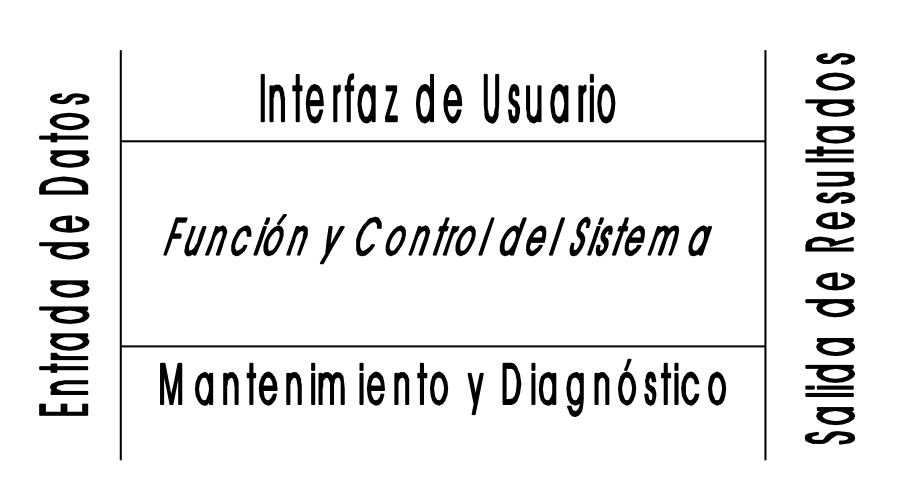
\includegraphics[width=0.6\linewidth]{Resources/Tema4/diagramaArquitectura.png}
    \caption{Diagrama de arquitectura de un sistema.}
\end{figure}

Si la complejidad del sistema lo requiere, puede formarse una jerarquía de niveles en la que el nivel superior se represente el sistema mediante un \uline{diagrama de contexto} (es el diagrama de arquitectura), y se irá detallando en sucesivos \uline{diagramas de flujo} (especifican el flujo de información en los subsistemas).

\begin{itemize}
    \item \textbf{Diagrama de contexto}: Representa el sistema en relación con su entorno, definiendo sus límites, y mostrando todos los productores y consumidores de información. Para ello, el sistema se encuentra en el centro del diagrama mientras que, a su alrededor, se sitúan las entidades o agentes externos, en sus correspondientes regiones, con los que se el sistema se relaciona mediante flujos de información.
        \begin{figure}[H]
            \centering
            \includegraphics[width=0.5\linewidth]{Resources/contextdiagram}
            \caption{Ejemplo de diagrama de contexto.}
            \label{fig:diagramaDeContexto}
        \end{figure}
    \item \textbf{Diagrama de flujo de arquitectura}: Determinan el flujo de entre los diferentes subsistemas a través de diagramas de flujo convencionales. Cada subsistema puede dar lugar a un diagrama de flujo, que pueden ser descompuestos a su vez en nuevos subsistemas, y ocupa una región del diagrama dependiendo de cuál sea su función (adquisición de datos, salida de datos, intefaz, etc.).
        \begin{figure}[H]
            \centering
            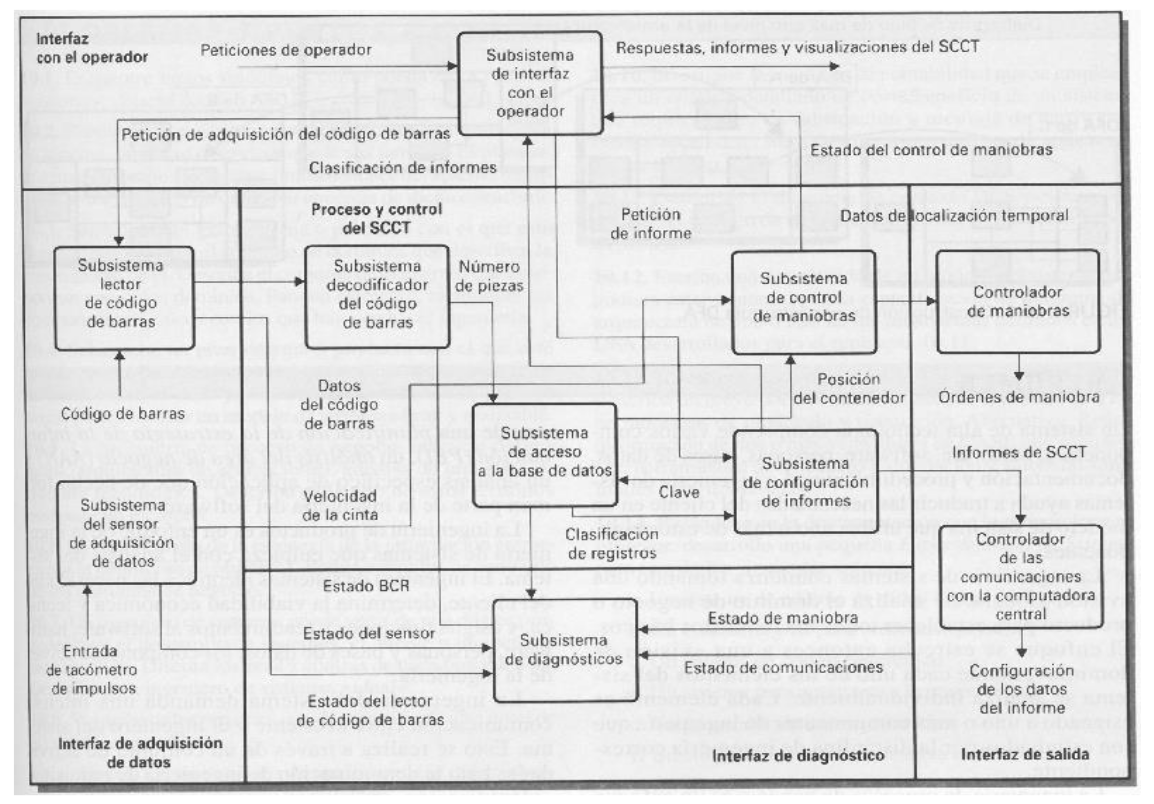
\includegraphics[width=0.8\linewidth]{Resources/Tema4/diagramaFlujo.png}
            \caption{Ejemplo de diagrama de contexto.}
            \label{fig:diagramaDeContexto}
        \end{figure}
\end{itemize}

\textbf{Nota:} \textit{Debe mantenerse la \uline{consistencia} entre los diagramas de distinto nivel. Al expandir un determinado subsistema en un diagrama de flujo, los flujos de información que conectan dicho subsitema con otros o con agentes externos deben figurar también. Estos flujos tendrán un extremo libre, que será el que los conectaba con dichos elementos que quedan fuera del ámbito del nuevo diagrama de flujo.
}

\section{Especificación del sistema}

Es un documento que sirve de base para analizar más adelante cada uno de los componentes que intervienen en el sistema, sean hardware, software o personas. Para ello, se describe \textbf{la función, rendimiento y restricciones que debe cumplir el sistema, limitando e indicando también el papel e interfaz de cada uno de sus compoentes}.\\

Este documento debería permitir al cliente comprobar si en análisis del ingeniero del sistema satisface sus necesidades, por lo que debe ser revisado de forma conjunta para comprobar si:

\begin{itemize}
    \item Se ha delimitado corectamente el ámbito del proyecto.
    \item Se han definido correctamente la funcionalidad, las interfaces y el rendimiento.
    \item Las necesidades del usuario y el análisis de riesgos justifican el desarrollo.
    \item El cliente y el analista tienen la misma percepción de los objetivos del proyecto.
\end{itemize}

Además de la evaluación con el usuario, debe realizarse una evaluación técnica para determinar si:

\begin{itemize}
    \item Las estimaciones de riesgos, coste y de agenda son correctas.
    \item Todos los detalles técnicos (funciones, interfaces\ldots) están bien definidos.
    \item La especificación sirve como base para las fases siguientes.
\end{itemize}

% La siguiente sección no aparece en las presentaciones ¿?
\section{Análisis de requisitos del software}

Como resultado de la fase de análisis de requisitos del sistema, el componente de software tiene ahora asignados una función y rendimiento. Es ahora tarea del ingeniero de software el desarrollar, o adquirir si existen alternativas en el mercado, los componentes software para ello.

\subsection{Objetivos y actividades}

El análisis de requisitos del software tiene como objetivo \textbf{desarrollar una representación del software que pueda ser revisada y aprobada por el cliente}, y que sirva de enlace entre la asignación de funciones al software realizada, y el posterior diseño del software.\\

Desde el punto de vista del analista de sistemas, esta fase \textbf{define con mayor precisión} las funciones y rendimiento del software, las interfaces con otros componentes y las restricciones que debe cumplir. Desde el punto de vista del diseñador, este análisis \uline{proporciona una representación} de la información, la función y el comportamiento del sistema que él se encargará de \uline{traducir en un diseño de datos y programas}. Además, el análisis de requisitos permite a todos, incluido el cliente, valorar la calidad del software una vez haya sido construido, o incluso antes de ello.\\

\textbf{Nota:} \textit{El analista debe centrarse en el \textbf{qué}, no en el \textbf{cómo}}.\\

\textit{Pressman} propone que el análisis de requisitos del software puede dividirse en cinco áreas:

\begin{itemize}
    \item \textbf{Inicialmente, el analista estudia la especificación del sistema para comprender el papel del software dentro de este}, para ir definiendo y refinando los flujos y la estructura de la información, la función del programa y su papel, así como las interfaces y restricciones.
    \item Con este conocimiento, \textbf{se proponen y evalúan diferentes soluciones al problema}, hasta que se acuerda una solución con el cliente, y se puede especificar así el software de forma adecuada para que se puedan efectuar las siguientes fases de desarrollo.
    \item La \textbf{síntesis de modelos} que se realiza, además de permitir entender mejor los flujos de información y la función de cada elemento del software, dará pie a modelos que sirvan de \textbf{base para el diseño de software}, así como que puedan ser empleados para la creación de prototipos.
    \item La \textbf{especificación del software debe indicar qué es lo que debe hacer}, pero no cómo debe hacerlo. Pueden figurar características como el rendimiento, protocolos, estándares, soporte de hardware\ldots
    \item Será necesario \textbf{revisar la especificación}, dado que inicialmente será un documento ambiguo, incompleto, incorrecto e inconsistente.
\end{itemize}

\subsubsection{Principios del análisis de requisitos del software}

Por una parte, los dos primeros puntos se refieren a representar el sistema y la información que maneja mediante diagramas o representaciones textuales; por otra parte, los dos últimos se refieren a un método de trabajo \textit{top-down}.

\begin{enumerate}
    \item \textbf{Identificar y representar el ámbito de información del sistema}: La tarea que realiza el software consiste siempre en procesar información, pero esta puede estar representada tanto por \textbf{datos} (información que procesa el sistema) como por \textbf{sucesos o eventos} (cuándo debe procesarse esa información). Así, el ámbito de información admite dos puntos de vista: flujo de datos y flujo de control; de todos modos, en ambos casos se requiere concretar el contenido de la información, su estructura y el flujo.
    \item \textbf{Modelar la información, la función y el comportamiento del sistema}: Se emplean \textbf{modelos de datos} (información que transforma el software), \textbf{modelos de procesos} (funciones que transforman la información) y \textbf{modelos de control} (comportamiento del sistema). Los modelos se utilizan para comprender mejor lo que se quiere construir, dado que:
          \begin{itemize}
              \item Ayudan al analista a entender la información, función y comportamiento del sistema.
              \item Sirven de base para el trabajo del diseñador.
              \item Sirven para validar el producto una vez desarrollado.
          \end{itemize}
    \item \textbf{Descomponer el problema de forma que se reduzca la complejidad}: Para abordar problemas que son demasiado grandes o complejos.
    \item \textbf{Avanzar desde lo más general a lo más detallado}: Descomponiendo un problema en subproblemas, y definiendo modelos sobre cada uno, conformando una jerarquía de modelos.
\end{enumerate}
% Fin de la sección


\section{Especificación del software}

La especificación del software es el documento que culmina el análisis de requisitos, conteniendo una \textbf{descripción detallada} del ámbito de información, funciones y comportamiento asignados al \textbf{software}, así como \textbf{información sobre requisitos} de rendimiento, restricciones diseño, y sobre las pruebas a realizar una vez se haya construido el software (de aceptación).

\subsection{Principios de especificación}

\textit{Pressman} propone los siguientes principios a seguir en la especificación del software:

\begin{enumerate}
    \item \textbf{Debe modelar el dominio del problema}: Debe describir el sistema tal y como es percibido por los expertos del dominio de aplicación.
    \item \textbf{Es necesario separar funcionalidad e implementación}: El \textit{qué}, y no el \textit{cómo}.
    \item \textbf{El lenguaje de especificación debe estar orientado al proceso}: El sistema debe considerar la posibilidad de modificar su comportamiento por interacturar en un entorno dinámico.
    \item \textbf{Debe abarcar todo el sistema del que el software es parte}: El comportamiento de una parte, como lo es el software, solo puede ser definido en el contexto del sistema completo.
    \item \textbf{Debe abarcar también el entorno del sistema}: Siguiendo el principio anterior. Permite además describir la interfaz del sistema, del mismo modo que sucede con las interfaces de los componentes del mismo.
    \item \textbf{La especificación debe ser operativa}: Debe servir para determinar si una implementación concreta la satisface.
    \item \textbf{Debe ser ampliable y tolerante a la incompletitud}: Al ser una especificación un modelo de un sistema real, nunca será completa (\textit{desde luego, será extremadamente difícil conseguirlo}), pero puede desarrollarse de forma incremental, a distintos niveles de detalle.
    \item \textbf{Debe estar localizada y débilmente acoplada}: La especificación sufrirá continuas modificaciones, por lo que su estructura debe facilitarlas todo lo posible. 
\end{enumerate}

\subsubsection{Características del documento de especificación}

En cambio, \textit{Piattini} propone una serie de características que debe cumplir la especificación para ser un documento útil:

\begin{enumerate}
    \item \textbf{No ambigua}: Cada característica del producto debe ser descrita con un término único y, en los casos en que un término se use en distintos contextos por distintos significados, debe incluirse un \textbf{glosario}. El uso del lenguaje natural implica un gran riesgo por su ambigüedad inherente.
    \item \textbf{Completa}: Una especificación de requisitos software (\textbf{ERS}) está completa si:
          \begin{itemize}
              \item Incluye todos los requisitos significativos del software.
              \item Define la respuesta software a todas las posibles entradas en todas las posibles situaciones.
              \item Está conforme con cualquier estándar de especificación que se deba cumplir.
              \item Están etiquetadas y referenciadas todas las tablas, figuras y diagramas del texto, y están definidos todos los términos y unidades de medida.
              \item No contiene la expresión \textit{TBD} (por determinar). Sin embargo, hay veces es necesario utilizarla, y debe acompañarse de:
                    \begin{itemize}
                        \item Una descripción de las condiciones que han causado el \textit{TBD}.
                        \item Una descripción de qué hay que hacer para eliminar el \textit{TBD}.
                    \end{itemize}
          \end{itemize}
    \item \textbf{Fácil de verificar}. Cualquier requisito al que hace referencia se puede verificar mediante algún procedimiento finito y efectivo en coste.
    \item \textbf{Consistente}: Si, y solo si, ningún conjunto de requisitos descritos en ella son contradictorios, total o parcialmente. Se pueden presentar tres tipos distintos de conflictos:
        \begin{itemize}
            \item Se define el mismo objeto real pero con distintos términos para designarlo.
            \item Las caracerísticas especificadas para objetos reales están en conflicto; \textit{por ejemplo, luces azules vs. luces verdes}.
            \item Hay un conflicto lógico o temporal entre dos acciones; \textit{por ejemplo, sumar dos valores vs. multiplicarlos.}
        \end{itemize}
    \item \textbf{Fácil de modificar}: Estar apropiadamente organizada, y no contener redundancia.
    
    \textbf{Nota:} \textit{La redundancia en sí no es un error, pero puede conducir fácilmente a ello. Es mejor emplear referencias cruzadas en su lugar.}
    \item \textbf{Facilidad para identificar el origen y las consecuencias de cada requisito}: De este modo, cuando se debe llevar a cabo una modificación, pueden determinarse claramente los requisitos que pueden verse afectados por ellas. Se consigue estableciendo la \uline{trazabilidad}.
    \item \textbf{Facilidad de utilización durante la fase de explotación y mantenimiento}:
        \begin{itemize}
            \item Si el personal que encarga del mantenimiento no ha estado relacionado con el desarrollo del producto, y debe llevar a cabo modificaciones ``profundas'', es necesario actualizar la documentación de diseño y de los requisitos. Por ello, además de que la ERS debería ser fácilmente modificable, debería contar con un registro de las características especiales de cada componente, como criticidad u origen, para facilitar dichos cambios; \textit{es decir, será mejor poder disponer de toda la información posible para evitar cometer errores.}
            \item Podría darse el caso de que parte de la información necesaria para el mantenimiento se dé por supuesta en la organización del desarrollo y, si la organización del mantenimiento no cuenta con ella, supondrá un gran problema.
        \end{itemize}
\end{enumerate}

\textbf{Nota:} \textit{Al igual que sucede con la especificación del sistema, la especificación de requisitos del software debe ser revisada conjuntamente por el cliente y el ingeniero del software. En primera instancia, debe determinarse si el sistema cumple, según el papel aquí especificado para el software, con la función, restricciones y rendimiento requeridos por el cliente, y ver si es necesario cambiar algunas de las estimaciones de coste, riesgo o agenda. En segundo lugar, debe realizarse una revisión mucho más detallada para detectar imprecisiones o ambigüedades en la especificación.}


\section{Verificación y Validación de requisitos}

La \textbf{validación de los requisitos es la que permite mostrar} (verificar) que éstos son los que \textbf{definen el sistema que el cliente desea}.\\

Presenta una relativa similitud con el análisis, ya que implica encontrar problemas con los requisitos, pero disciernen en que la validación comprende un bosquejo completo del documento de requisitos, mientras que el análisis implica trabajar con requisitos incompletos.

\subsection{Estrategias}

Durante el proceso de validación, deben llevarse a cabo diferentes tipos de comprobaciones sobre los requisitos:

\begin{enumerate}
    \item \textbf{Comprobación de validez}. Dado que cada sistema tendrá sus propias necesidades, ¿la especificación responde a todas las necesidades del proyecto? \textit{Por ejemplo, es posible que se identifique una necesidad de contar con determinadas funciones adicionales a medida que los analistas comprenden mejor el sistema que el cliente desea.}
    \item \textbf{Comprobación de consistencia}: Los requisitos en el documento no deben contradecirse.
    \item \textbf{Comprobación de totalidad}: Se deben incluir requisitos que definan todas las funciones y restricciones propuestas para el sistema.
    \item \textbf{Comprobación de realismo}: Asegurar que los requisitos puedan implementarse actualmente, y teniendo en cuenta además restricciones de presupuesto y calendarización.
    \item \textbf{Verificabilidad}: Debe ser posible diseñar un conjunto de verificaciones (pruebas) para demostrar que el sistema a entregar cumple los requisitos.
\end{enumerate}

\subsection{Técnicas}

Las técnicas dictan cómo llevar a cabo las estrategias:

\begin{enumerate}
    \item \textbf{Revisiones de requisitos}: Varios implicados, pertenecientes tanto al cliente como al contratista, llevan a cabo un proceso de análisis sistemático del documento de requisitos para encontrar anomalías y omisiones.
    \item \textbf{Construcción de prototipos}: Se muestra un modelo ejecutable del sistema a los usuarios finales para que experimenten y comprueben si cumple sus necesidades.
    \item \textbf{Generación de casos de prueba}. Los requisitos deben poder probarse. Si una prueba es difícil o imposible de diseñar, suele significar que los requisitos serán difíciles de implementar, por lo que deben ser reconsiderados.
    \item \textbf{Análisis de consistencia automática}. Si los requisitos se expresan en una notación estructurada o formal.
\end{enumerate}

\textbf{Nota:} \textit{No deben menospreciarse las dificultades en la validación de requisitos, dado que es difícil demostrar que un conjunto de requisitos cumple las necesidades del usuario, por requerir visualizar cómo el sistema final encajaría en su entorno de explotación; esto será complejo para los profesionales de la computación, pero aún más para los usuarios. Por ende, la validación de requisitos probablemente descubrirá todos los problemas en las interpretaciones realizadas sobre las necesidades del cliente, y será inevitable corregir todos estos problemas.}


\section{Administración de requisitos}

La \textbf{ERS habitúa ser un proceso iterativo}, como consecuencia del progreso del producto de software; a fin de cuentas, es \textbf{casi imposible especificar algunos detalles en el momento que se inicia el proyecto}. También es muy probable que se realicen cambios adicionales como resultado de haber encontrado deficiencias.\\

Dos consideraciones a tener en cuenta en este proceso son:

\begin{itemize}
    \item Especificar los requisitos de la forma más completa posible, a pesar de que se prevean de forma inevitable revisiones en él.
    \item Debe iniciarse un proceso de gestión formal del cambio, para identificar, controlar, seguir e informar de posibles cambios tan pronto como sean identificados. De este modo, se podrá contar con un rastro preciso de las modificaciones de la ERS, así como discernir entre los fragmentos actuales de la ERS y sus anteriores versiones.
\end{itemize}

Como se puede ver, la administración de requisitos es el proceso de comprender y controlar los cambios en los requisitos del sistema. Consta de \textbf{dos etapas}: la planificación debería comenzar al mismo tiempo que la obtención de requisitos inicial, y la administración activa debe comenzar tan pronto como esté lista la primera versión del documento de requisitos.

\subsection{Clasificación cualitativa}

Desde una perspectiva evolutiva, los requisitos son de una de las siguientes dos clases:

\begin{itemize}
    \item \textbf{Requisitos duraderos}: Relativamente estables dado que derivan de la actividad de la organización y, por lo tanto, están relacionados directamente con el dominio del sistema. \textit{Por ejemplo, en un hospital siempre habrá pacientes, doctores\ldots}
    \item \textbf{Requisitos volátiles}: Probablemente cambiarán durante el desarrollo del sistema o después de que se haya puesto en operación. \textit{Por ejemplo, por cambios en las políticas gubernamentales de salud}.
    
    \textit{Sommerville} clasifica estos últimos en:
    \begin{itemize}
        \item \textbf{Cambiantes}: Debido al ambiente en que opera la organización.
        \item \textbf{Emergentes}: Surgen al incrementarse la compresión del cliente en el desarrollo del sistema; dicho de otro modo, \textit{se entiende más sobre lo que el cliente desea}.
        \item \textbf{Consecutivos}: Son resultado de la introducción del sistema en su entorno de explotación (puede suponer cambios en los procesos de la organización).
        \item \textbf{De compatibilidad}: Dependen de sistemas particulares o procesos de negocios dentro de la organización.
    \end{itemize}
\end{itemize}

\subsection{Clasificación cuantitativa}

Desde otro punto de vista, simplemente pueden clasificarse asignándoles el \textbf{valor de estabilidad} que se considere apropiado: baja, media y alta.

\subsection{Planificación de la administración de requisitos}

La administración de requisitos es muy cara, por lo que es necesario definir en todo proyecto el nivel de detalle necesario para este proceso. Para ello, deben concretarse los siguientes aspectos:

\begin{itemize}
    \item \textbf{La identificación de requisitos}: Cada requisitos debe ser identificable de forma unívoca.
    \item \textbf{Un proceso de administración del cambio}: Conjunto de actividades que evalúan el impacto y costo de los cambios.
    \item \textbf{Políticas de rastreo}: Definen las relaciones entre requisitos dependientes, entre requisitos y los módulos del diseño en los cuales serán implementados, y entre los requisitos y sus fuentes (quién y por qué se propusieron). Esto permite que, cuando un cambio sea propuesto, se pueda rastrear el impacto en los requisitos y en el diseño, de modo que se pueda valorar si proceder a realizar el cambio o no.
    \item \textbf{Ayuda de herramientras CASE} (\textit{Computer Aided Software Engineering}).
\end{itemize}

\textbf{Nota:} \textit{Es habitual registrar esta información de rastreo mediante matrices de rastreo. Además, la administración de requisitos idealmente recurrirá a la ayuda de herramientas CASE para almacenarlos, y administrar sus cambios y trazabilidad.}

\subsection{Administración del cambio de requisitos}

Esta administración se aplica a todos los cambios propuestos en los requisitos. La ventaja de emplear un proceso formal es que todos los cambios propuestos son tratados \textbf{de forma consistente} y que los cambios en el documento de requisitos se realizan \textbf{de forma controlada}.\\

\textbf{Nota:} \textit{La gestión del cambio es un proceso aparte para todos los artefactos del proyecto, pero los primeros sobre los que se aplica son los requisitos.}\\

Existen tres etapas principales:

\begin{itemize}
    \item \textbf{Análisis del problema y especificación del cambio}: Tras \textbf{identificar un problema}, o a veces recibir una \textbf{propuesta de cambio}, se analiza la información correspondiente para verificar que es válida y, entonces, se hace una propuesta de cambio de requisitos más específica.
    \item \textbf{Análisis del cambio y costeo}: Se valora el efecto de un cambio propuesto empleado la información de rastreo y el conocimiento general de los requisitos del sistema. Finaliza con la toma de decisión de si procede o no el cambio.
    \item \textbf{Implementación del cambio}: Se modifica el documento de requisitos y, si procede, el diseño e implementación del sistema.
\end{itemize}

En caso de que se requiera de forma urgente un cambio en los requisitos del sistema, existirá la tentación de hacer el cambio del sistema y de modificar el documento tras ello. Esto conduce, inevitablemente, a que la especificación de requisitos y el sistema se desfasen, de modo que no sean consistentes el uno con el otro por, por ejemplo, posponer la actualización del documento.

\newpage
\part{Análisis estructurado}

\section{Introducción}

\paragraph{Modelo} Descripción simplificada del sistema, que se utiliza en el análisis de requisitos como herramienta sobre la que trabajar con el cliente para construir un sistema adecuado a sus necesidades.\\

Todos los métodos de análisis de requisitos se basan en la construcción de modelos del sistema que se pretende desarrollar, los cuales \textbf{lo reflejan}, mediante la aplicación de \textbf{técnicas de descomposición y de razonamiento \textit{top-down}}. El desarollo de modelos presenta claras \uline{ventajas} como:

\begin{itemize}
    \item \textbf{Ayudar a entender y corregir}:
    \begin{itemize}
        \item Permiten centrarse en determinadas características del sistema.
        \item Permiten realizar cambios y correcciones en los requisitos a bajo coste y sin correr ningún riesgo. Si no se realizasen modelos, estos cambios solo se efectuarían después de construir el producto software.
    \end{itemize}
    \item \textbf{Ayudar a representar y transmitir}:
    \begin{itemize}
        \item Permiten verificar que el ingeniero del software ha entendido correctamente las necesidades del usuario, y que las ha documentado de forma que los diseñadores y programadores puedan construir el software.
    \end{itemize}
    \item \textbf{Ayudar en el proceso de reflexión} (\textit{feedback}):
    \begin{itemize}
        \item Permiten comprobar la correcta realización de cada fase determinando si verifican o no los modelos.
    \end{itemize}
\end{itemize}

\subsection{Problemas del análisis clásico}

No todas las técnicas de análisis logran estos objetivos. Por ejemplo, una descripción del sistema de 500 páginas ocultará características del sistema, tendrá un desarrollo enormemente costoso, y será difícil de modificar, entre otros motivos.\\

Esto se ve claramente reflejado en el análisis de requisitos clásico, usado hasta finales de los 70. Este consistía en redactar especificaciones funcionales, en forma de documentos de texto que eran:

\begin{enumerate}
    \item \textbf{Monolíticos}: Había que leerlos de principio a fin.
    \item \textbf{Redundantes}: Lo cual suele inducir a inconsistencias en caso de querer hacer cambios.
    \item \textbf{Ambiguas}: Por el uso del lenguaje natural.
    \item \textbf{Imposibles de mantener o modificar}: Al ser redundantes, cualquier modificación de una parte podía provocar una inconsistencia, obligando a leer todo el documento debido a que era una ``unidad monolítica''.
\end{enumerate}

Es por ello que la mayor parte del software de la época carece de documentación fiable.

\subsection{Soluciones al análisis clásico}

Como consecuencia, fueron surgiendo nuevos métodos de análisis con los que obtener especificaciones:

\begin{enumerate}
    \item \textbf{Gráficas}: Diagramas acompañados de información textual detallada. Sirven únicamente como material de referencia, y no de cuerpo principal de la especificación.
    \item \textbf{Particionadas}.
    \item \textbf{Mínimamente redundantes}.
    \item \textbf{Transparentes}: Fáciles de leer y comprender.
\end{enumerate}

%Lo siento mucho almuiña pero aquí es probable que pregunte por siglas
\section{Técnicas de especificación y modelado}

El análisis estructurado \textbf{propone la descripción de los sistemas según 3 puntos de vista} (como si fuesen tres dimensiones del espacio):

\begin{enumerate}
    \item \textbf{Punto de vista de los datos (dimensión de la información)}: Se centra en la información que utiliza el sistema, representando el modelo de los datos usados, así como las relaciones entre ellos.
          \begin{itemize}
              \item \textbf{D}iagramas \textbf{E}ntidad--\textbf{R}elación (\textbf{DER}).
              \item \textbf{D}iagramas \textbf{E}structura de \textbf{D}atos (\textbf{DED}).
          \end{itemize}
    \item \textbf{Punto de vista del proceso (dimensión de la función)}: Se centra en qué hace el sistema, describiendo el conjunto de operaciones que reciben flujos de datos de entrada, y los transforman en flujos de datos de salida.
          \begin{itemize}
              \item \textbf{D}iagramas de \textbf{F}lujo de \textbf{D}atos (\textbf{DFD}).
              \item \textbf{Especificaciones de Procesos} (\textbf{PSPECs}): Término genérico que engloba la definición de cómo un sistema transforma unas entradas en salidas mediante pseudocódigo, lenguaje natural, diagramas de flujo\ldots
          \end{itemize}
    \item \textbf{Punto de vista del comportamiento (dimensión del tiempo)}: Se centra en cuándo sucede algo en el sistema, modelando el sistema como una sucesión de estados o modos de funcionamiento, así como se indica cuáles son las condiciones o eventos que hacen que el sistema pase de un modo a otro.
          \begin{itemize}
              \item \textbf{D}iagramas de \textbf{F}lujo de \textbf{C}ontrol (\textbf{DFC}).
              \item \textbf{Especificaciones de Control} (\textbf{CSPECs}).
              \item Diagramas de Estados.
              \item Redes de Petri.
          \end{itemize}
\end{enumerate}

\textbf{Nota:} \textit{Todos los modelos describen el mismo sistema, pero desde distintos puntos de vista. Por ende, debe asegurarse la consistencia ellos.}\\

Cada sistema en particular tendrá una \uline{representación de mayor o menor importancia para cada una de estas dimensiones}. Por ejemplo, un sistema de información basado en una gran base de datos, tendrá una importante componente en la dimensión de la información; un sistema de gestión en tiempo real, tendrá mayor peso en la dimensión del tiempo; y un sistema de simulación, hará mayor énfasis en la dimensión de la función.\\

Al final, \textbf{cada modelo se centra en un número limitado de aspectos del sistema}, dejando de lado otros, y será necesario \textbf{combinar todos los que se consideren necesarios para tener una visión detallada} de todas las características del sistema.\\

Por otra parte, la relación entre los diagramas de cada dimensión se establece con las técnicas que representan los planos formados por cada dos dimensiones.\\

En la tabla siguiente se representa una posible clasificación de las \uline{técnicas de modelado} según su/sus dimensiones; las que tengan la misma fila y columna, se centrarán en una dimensión, mientras que las otras harán referencia al plano formado por las dos dimensiones indicadas por su fila y columna.

\begin{table}[ht]
    \centering
    \resizebox{\textwidth}{!}{
        \begin{tabular}{c|l|l|l|} \cline{2-4}
                                                                        & \multicolumn{1}{c|}{\textbf{Información}} & \multicolumn{1}{c}{\textbf{Función}} & \multicolumn{1}{|c|}{\textbf{Tiempo}} \\ \hline

            \multicolumn{1}{|c|}{\multirow{4}{*}{\textbf{Información}}} & D. entidad--relación                      &                                      &                                       \\
            \multicolumn{1}{|c|}{}                                      & D. de estructura de datos                 &                                      &                                       \\
            \multicolumn{1}{|c|}{}                                      & Matriz entidad/entidad                    &                                      &                                       \\
            \multicolumn{1}{|c|}{}                                      & D. de clases                              &                                      &                                       \\ \hline

            \multicolumn{1}{|c|}{\multirow{7}{*}{\textbf{Función}}}     & D. de flujo de datos                      & D. de flujo de datos                 &                                       \\
            \multicolumn{1}{|c|}{}                                      & Matriz función/entidad                    & D. de casos de uso                   &                                       \\
            \multicolumn{1}{|c|}{}                                      & D. de clases                              & D.de estructura de datos             &                                       \\
            \multicolumn{1}{|c|}{}                                      & D. de colaboración                        & Tarjetas CRC                         &                                       \\
            \multicolumn{1}{|c|}{}                                      &                                           & D. de componentes                    &                                       \\
            \multicolumn{1}{|c|}{}                                      &                                           & D. de despliegue                     &                                       \\
            \multicolumn{1}{|c|}{}                                      &                                           & D. de actividad                      &                                       \\ \hline

            \multicolumn{1}{ |c| }{\multirow{4}{*}{\textbf{Tiempo}}}    & D. de historia y vida de la entidad       & Redes de Petri                       & D. de flujo de control                \\
            \multicolumn{1}{|c|}{}                                      & D. de estados                             & D. de estados                        & D. de estados                         \\
            \multicolumn{1}{|c|}{}                                      & D. de secuencia                           & D. de secuencia                      &                                       \\
            \multicolumn{1}{|c|}{}                                      &                                           & D. de actividad                      &                                       \\ \hline
        \end{tabular}
    }
    \caption{Diferentes técnicas de modelado}
\end{table}

Dichas técnicas buscan modelar a alto nivel el sistema en cada una de sus dimensiones.\\

Las siguientes técnicas dan el máximo nivel de detalle posible de aquel aspecto que representan, por lo que se conocen como \uline{técnicas de especificación}.

\begin{table}[ht]
    \centering
    \resizebox{\textwidth}{!}{
        \begin{tabular}{c|l|l|l|} \cline{2-4}
                                                                        & \multicolumn{1}{c|}{\textbf{Información}} & \multicolumn{1}{c}{\textbf{Función}} & \multicolumn{1}{|c|}{\textbf{Tiempo}} \\ \hline

            \multicolumn{1}{|c|}{\multirow{1}{*}{\textbf{Información}}} & Especificación de entidad                      &                                      &                                       \\ \hline

            \multicolumn{1}{|c|}{\multirow{3}{*}{\textbf{Función}}}     &                                           & Diccionario de datos                 &                                       \\
            \multicolumn{1}{|c|}{}                                      &                                           & Especificación de procesos                   &                                       \\
            \multicolumn{1}{|c|}{}                                      &                                           & Especificación de entidades externas            &                                       \\ \hline

            \multicolumn{1}{ |c| }{\multirow{1}{*}{\textbf{Tiempo}}}    &                                           & Definición de función                       & Especificación de eventos                \\ \hline
        \end{tabular}
    }
    \caption{Diferentes técnicas de especificación}
\end{table}


\subsection{Diagramas de flujo de datos (DFD, Función--Información, Función--Función)}

Surgen como respuesta a la necesidad de describir:

\begin{itemize}
    \item \textbf{Qué funciones} son las que realiza el sistema.
    \item \textbf{Qué interacción} se produce entre estas funciones: A dónde va la información de salida de una determinada función.
    \item \textbf{Qué transformaciones de datos} realiza el sistema, especificando \textbf{qué datos de entrada se transforman en qué datos de salida}: Qué se convierte en qué, y por dónde va.
\end{itemize}

Así, el \textbf{DFD} representa el \uline{flujo de información} y las \uline{transformaciones} que se aplican a los datos al moverse desde la entrada a la salida. Dicho de otro modo, se representa el sistema desde un \textbf{punto de vista funcional}; esto es, las \textbf{entidades básicas son funciones o procesos} que transforman unos datos de entrada en salidas, y el sistema resulta ser el flujo de información a través de estas funciones.\\

Los DFD \textbf{NO} representan el \textbf{comportamiento del sistema}, ni el \textbf{control del mismo}; es decir, solo dicen lo que hace el sistema pero \textbf{NO} indican:

\begin{enumerate}
    \item \textbf{Cuándo se hace}.
    \item \textbf{En qué secuencia se hace}.
\end{enumerate}

\subsubsection{Elementos}

\begin{figure}[H]
    \centering
    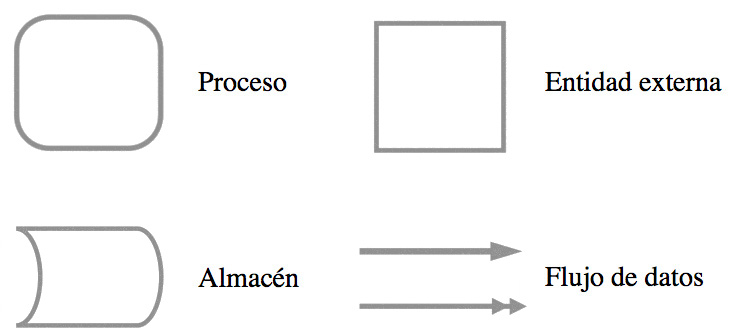
\includegraphics[width=0.5\linewidth]{Resources/Tema5/elementosDFD.jpg}
    \caption{Notación utilizada para representar los elementos del DFD.}
    \label{fig:elementosDFD}
\end{figure}
\begin{enumerate}
    \item \textbf{Procesos}: Representan elementos software que \uline{transforman información}; por ende, son los componentes del software que realizan cada una de las \uline{funciones del sistema}. Deben verificar las siguientes \uline{reglas}:
    \begin{itemize}
        \item \textbf{De conservación de datos}: El proceso debe ser capaz de generar las salidas a partir de los flujos de entrada más una posible información local.
        \item \textbf{Pérdida de información}: Todas las entradas del proceso tienen que emplearse para calcular alguna de sus salidas.
    \end{itemize}

    \item \textbf{Entidades externas}: Representan elementos del sistema informático o de otros sistemas adyacentes (en todo caso, fuera del los límites del sistema software) que producen información que será transformada por el software, o consumen la resultante. Los flujos de datos que comunican el sistema con las entidades externas representan las interfaces del sistema. \textbf{Sólo aparecen en el diagrama de contexto}, y los flujos entre unidades externas no son objeto de estudio.

    \item \textbf{Almacenes de datos}: Representan información almacenada que puede ser utilizada por el software; concretamente, permiten guardar de forma temporal información que será consumida, o bien por el mismo proceso que la creó, o bien por otro distinto; en la mayoría de los casos, utilizaremos almacenes de datos cuando los \uline{procesos intercambien información pero no estén sincronizados}. Se pueden representar múltiples veces para una mayor legibilidad, y no pueden existir comunicaciones entre almacenes.

    \item \textbf{Flujos de datos}: Representan \uline{datos o colecciones de datos que fluyen a través del sistema}, conectando los procesos con otros procesos, con entidades externas o con almacenes de datos. Posiblemente, en los diagramas de nivel mayor existirán flujos de datos bidireccionales (\uline{par de diálogo}), o incluso varios flujos de datos agrupados en uno solo (\uline{flujos múltiples}), que serán refinados en sucesivos diagramas. Contienen información de las tres dimensiones, aunque normalmente sólo representan las dimensiones de Función e Información. Aún así cabe destacar que, según su \textbf{dimensión temporal}, los flujos pueden ser:
          \begin{enumerate}[a.]
              \item \textbf{Discretos} \textit{(flecha con una cabeza)}: Representan movimiento de datos en un instante determinado de tiempo.
              \item \textbf{Continuos} \textit{(flecha con con dos cabezas)}: Implican una transmisión continua de información; \textit{por ejemplo, comprobar si un registro ha cambiado}.
          \end{enumerate}
\end{enumerate}

\textbf{Nota:} \textit{La comunicación entre almacenes y entidades externas solo se representará excepcionalmente cuando el almacén haga de interfaz con la entidad.}

\begin{figure}[h!]
    \centering
    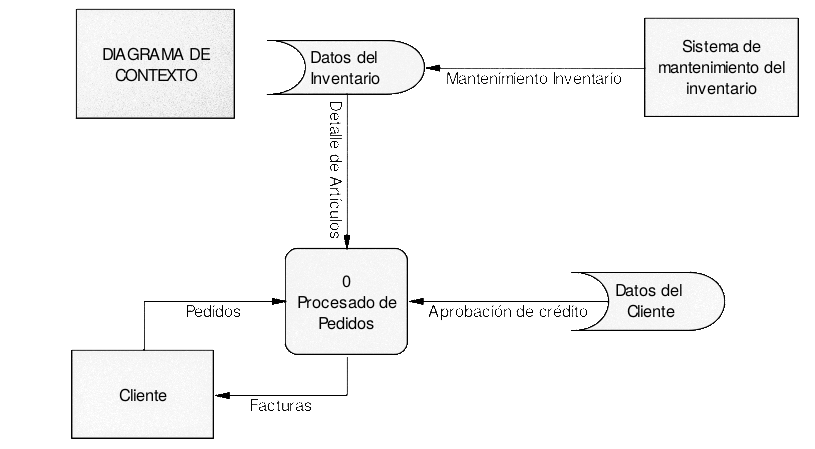
\includegraphics[width=0.8\linewidth]{Resources/Tema5/ejemploDFDInterfazAlmacen.png}
    \caption{Ejemplo de un Diagrama de Flujo de Datos en el que un almacén actúa de interfaz con una entidad.}
    \label{fig:ejemploDFDInterfazAlmacen}
\end{figure}

Cualquiera de los elementos de un DFD tiene que estar etiquetado con un nombre significativo y único:

\begin{itemize}
    \item Los procesos y entidades externas se etiquetan con la función que realizan.
    \item Los flujos de datos se etiquetan con un nombre identificativo de la información, e incluso su estado. \textit{Por ejemplo, número de teléfono, número de teléfono correcto, número de teléfono incorrecto\ldots}
    \item Los almacenes de datos se etiquetan con un nombre significativo de la información contenida, generalmente en plural.
\end{itemize}

\subsubsection{Niveles}

Los \textbf{DFD} permiten la representación del sistema en múltiples niveles de abstracción, de modo que se pueden representar gráficos con un número reducido de procesos (como máximo 7$\pm$2), y con un límite ideal de 7--8 niveles; si fuese necesario emplear más niveles, o bien la complejidad del sistema sería muy alta, o bien el desarrollador está descomponiendo demasiado sus características. Cabe distinguir:

\begin{enumerate}
    \item \textbf{Nivel 0}: \textbf{Diagrama de Contexto}.\\
          Representa el sistema como un único proceso, el \textbf{proceso 0}, que realiza la función principal del sistema, como si de una \uline{caja negra} se tratase. Se representan también las entidades que interactúan con el mismo, dejando claros los \textbf{límites del sistema}, así como sus \textbf{interfaces}.\\
          
          A partir de este diagrama de contexto, se pueden ir construyendo nuevos diagramas que vayan \textbf{definiendo con mayor nivel de detalle el sistema} ya que, en general, un proceso que aparezca en un DFD puede ser descrito más detalladamente con un nuevo DFD; a este procedimiento se le llama \uline{explosión de un proceso}. Así, el proceso aparece descompuesto en una serie de subprocesos o subsistemas. Los flujos de datos que entraban y salían del proceso deben hacerlo también del DFD que lo desarrolla, y este contendrá por lo general nuevos flujos que comunican los procesos que figuren en él, y posiblemente almacenes de datos.\\

          \textbf{Nota:} \textit{Las entidades externas solo aparecen, por lo tanto, en el DFD de contexto.}

          %Imagen nivel 0
          \begin{figure}[h!]
              \centering
              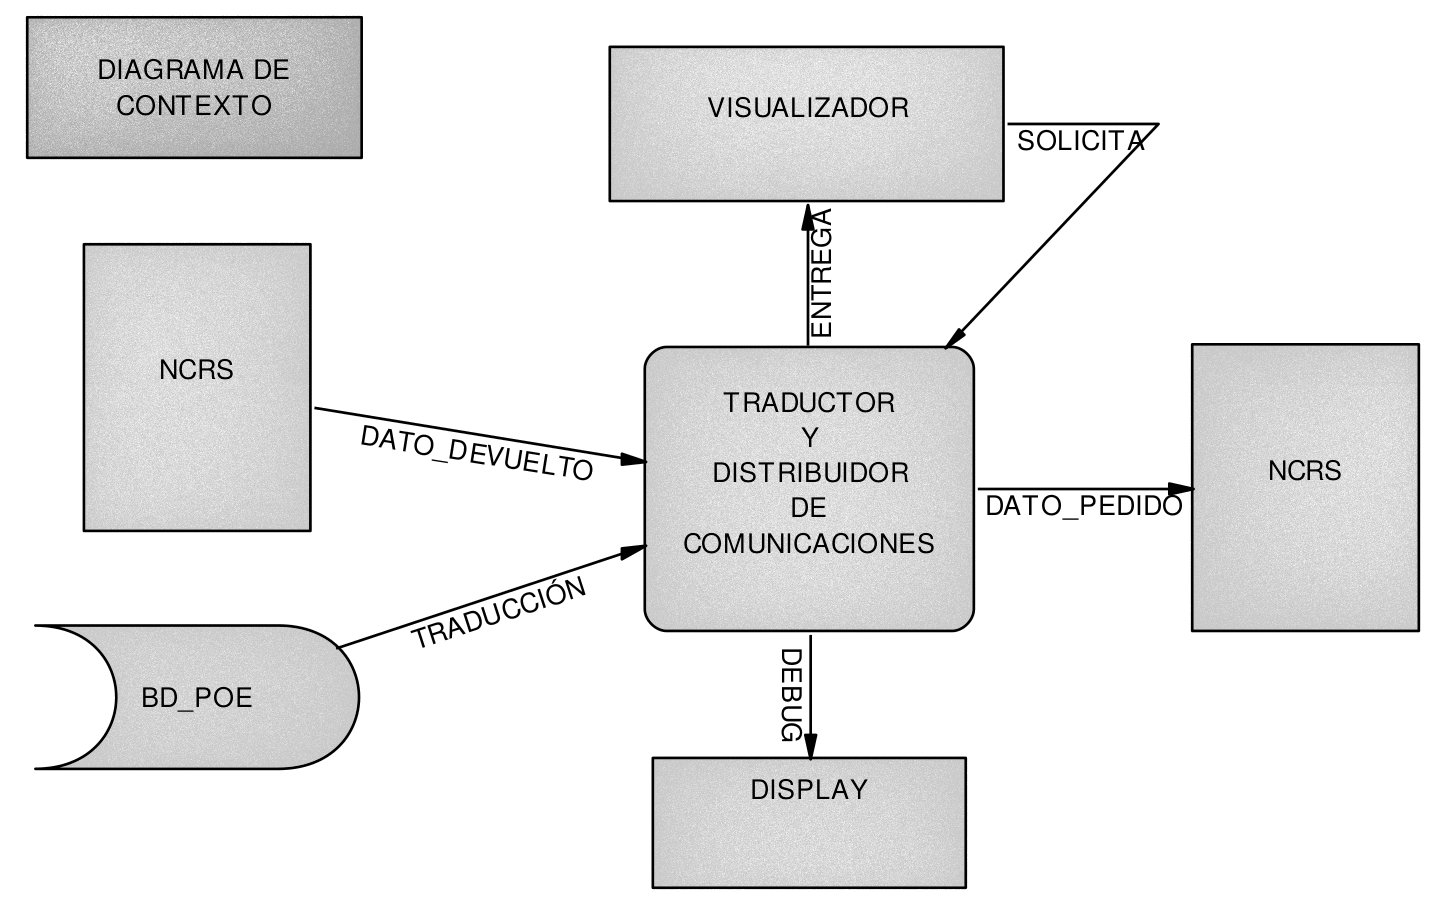
\includegraphics[width=0.7\linewidth]{Resources/Tema5/nivel0.png}
              \caption{DFD de nivel 0 de un Traductor y Distribuidor de Comunicaciones (TDC).}
              \label{fig:dfdn0}
          \end{figure}
    \item \textbf{Nivel 1}: \textbf{Diagrama 0} o \textbf{de Sistema}.\\
          Denominado así por \textit{descomponer el proceso 0} en sus funciones principales; es interesante que éstas sean \textit{independientes} y que procesen \textit{los mismos flujos} que el de nivel 0.
          %Imagen nivel 1
          \begin{figure}[h!]
              \centering
              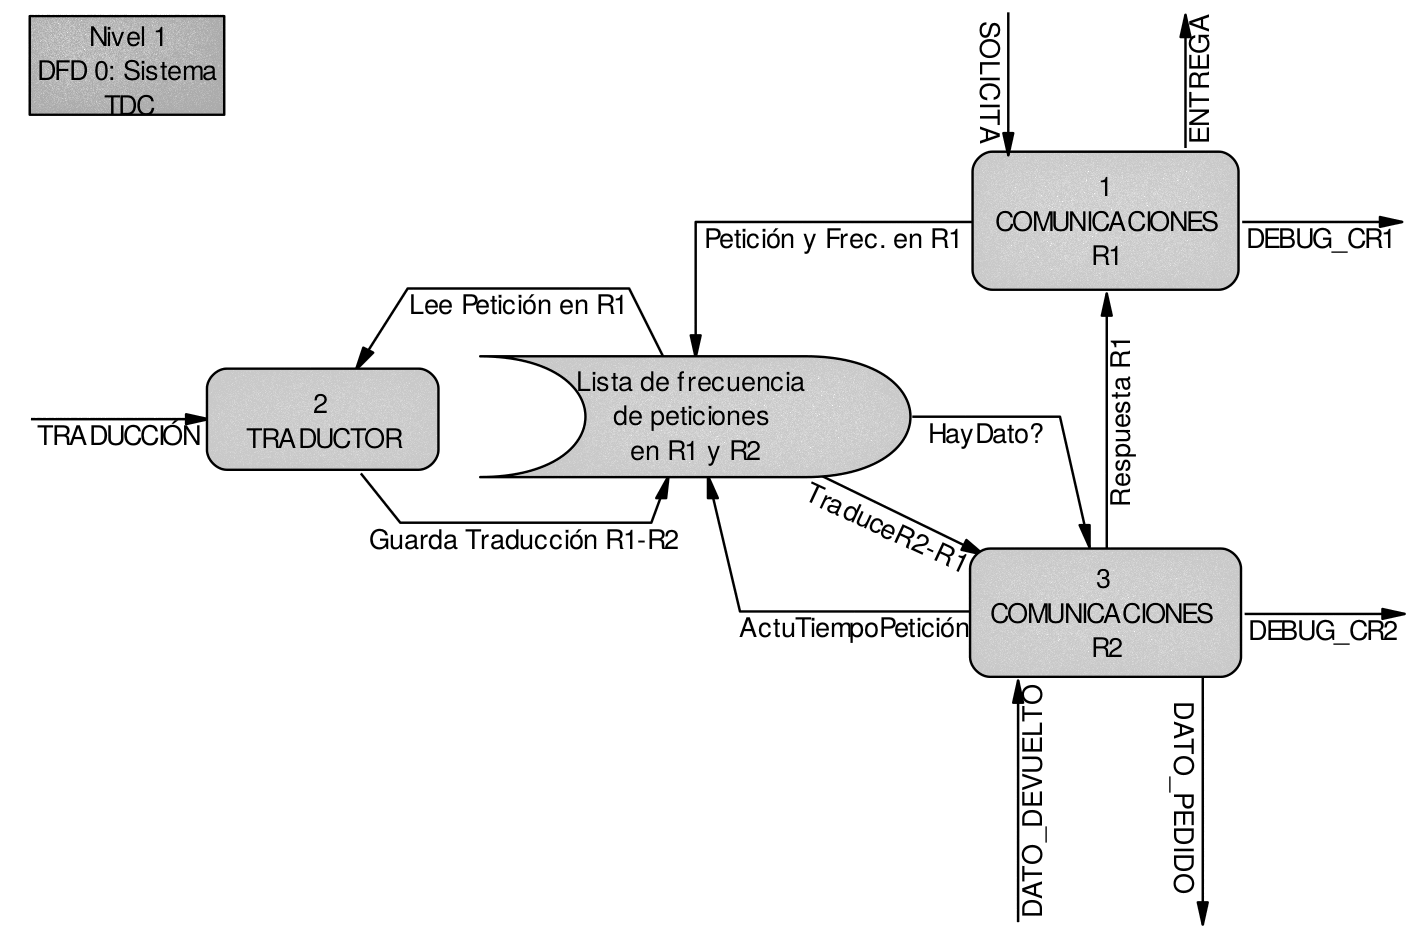
\includegraphics[width=0.7\linewidth]{Resources/Tema5/nivel1_DFD.png}
              \caption{DFD de nivel 1 del TDC. Nótense los flujos de control \textit{DEBUG\_CR1} y \textit{DEBUG\_CR2}, que denotan que procedían de un flujo compuesto situado en un diagrama antecesor.}
              \label{fig:dfdn1}
          \end{figure}
    \item \textbf{Niveles 2...N--1}\\
          Se continúa descomponiendo los procesos en subprocesos, recogiendo las interfaces (flujos) de nivel superior y asignándoselas a subprocesos.
          %Imagen nivel 2
          \begin{figure}[h!]
              \centering
              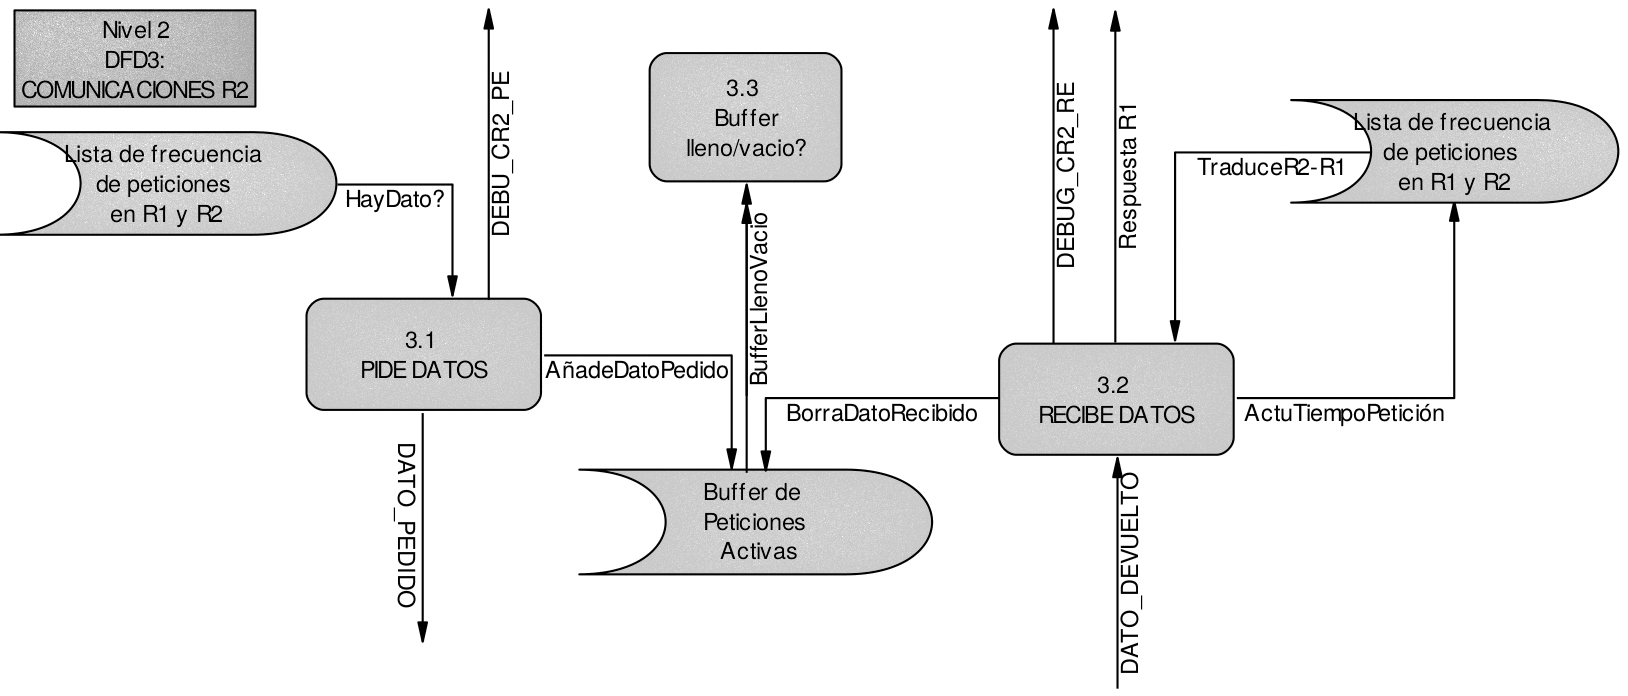
\includegraphics[width=0.7\linewidth]{Resources/Tema5/nivel2_Proceso3_DFD.png}
              \caption{DFD de nivel 2 del proceso $3$ del TDC.}
              \label{fig:dfdn2}
          \end{figure}
    \item \textbf{Nivel N}\\
          Contiene los procesos primitivos, que no se pueden descomponer. Para describirlos, deben emplearse técnicas de especificación de procesos.
    \item \textbf{Procesos primitivos}
\end{enumerate}

\textbf{Nota:} \textit{Como se puede observar, un DFD puede dar lugar, como máximo, a tantos DFDs como procesos contenga.}\\

La descomposición de un sistema en diferentes niveles (jerarquía de DFDs) debe respetar la \uline{regla del balanceo}. Sus restricciones pueden separarse en dos partes.\\

En primer lugar, los procesos en el DFD tienen un \textbf{identificador numérico} de modo que:
\begin{itemize}
    \item Nivel 0: Solo contiene un proceso, el \textbf{``0''}
    \item Nivel 1: Se le asigna a cada proceso un número secuencialmente, \textbf{\{1, 2, 3\ldots\}}
    \item Niveles 2...N: La numeración de los procesos en el DFD hijo se deriva del número del DFD padre; \textit{por ejemplo, para el proceso 3, serían 3.1, 3.2\ldots}
\end{itemize}

Por otra parte:

\begin{itemize}
\item El título del DFD hijo debe ser el nombre del proceso que desarrolla.
\item Debe mantenerse la \textbf{consistencia de los flujos de datos entre los DFDs} padre e hijo. En el diagrama hijo, estos flujos tendrán un extremo libre, puesto que conectaban el proceso padre con algún elemento que ya no va a estar representado; una excepción son los flujos que conectan los procesos con los almacenes de datos.
\end{itemize}

De todos modos, esta regla del balanceo puede contener excepciones. Un ejemplo de ello lo son los flujos de datos bidireccionales y los compuestos, dado que cada uno de estos deberá descomponerse en algún momento en varios flujos.

\subsection{Especificaciones de proceso (PSPEC)}

Los DFDs no indican nada acerca de los detalles de cómo se realizan las transformaciones en el sistema. Es aquí en donde entra en juego la \textbf{P}rocess \textbf{Spec}ification, que es un documento que describe textualmente los detalles de un proceso, indicando \textbf{cómo es el procedimiento de transformación de una información de entrada en otra de salida}; dicho de otro modo, debe definir, de forma más o menos formal, cómo se obtienen los flujos de salida a partir de los de entrada más una posible información local.\\

Para generar estos documentos, los procesos de los DFDs de menor nivel (más altos en la jerarquía) se irán describiendo mediante nuevos DFDs, hasta alcanzar un nivel en el que un proceso pueda ser descrito textualmente de forma sencilla y no ambigua; estos procesos suelen llamarse \textbf{procesos primitivos}. De este modo, las PSPEC servirán para complementar los DFDs.\\

Las descripciones de estos procesos deben:

\begin{itemize}
    \item Ser \textbf{breves} (menos de una página).
    \item Incluir \textbf{precondiciones} y \textbf{postcondiciones}.
\end{itemize}

Y, para su elaboración, se utilizan diferentes \uline{técnicas de especificación}:

\begin{enumerate}
    \item Lenguaje natural; \textit{por ejemplo, mediante una definición como ``invertir una matriz''}.
    \item Diagramas de flujo.
    \item Lenguaje estructurado, y diagramas de acción (pseudocódigo, especificar un algoritmo). 
    \item Árboles de decisión.
    \item Tablas de decisión.
\end{enumerate}

\begin{figure}[h!]
    \centering
    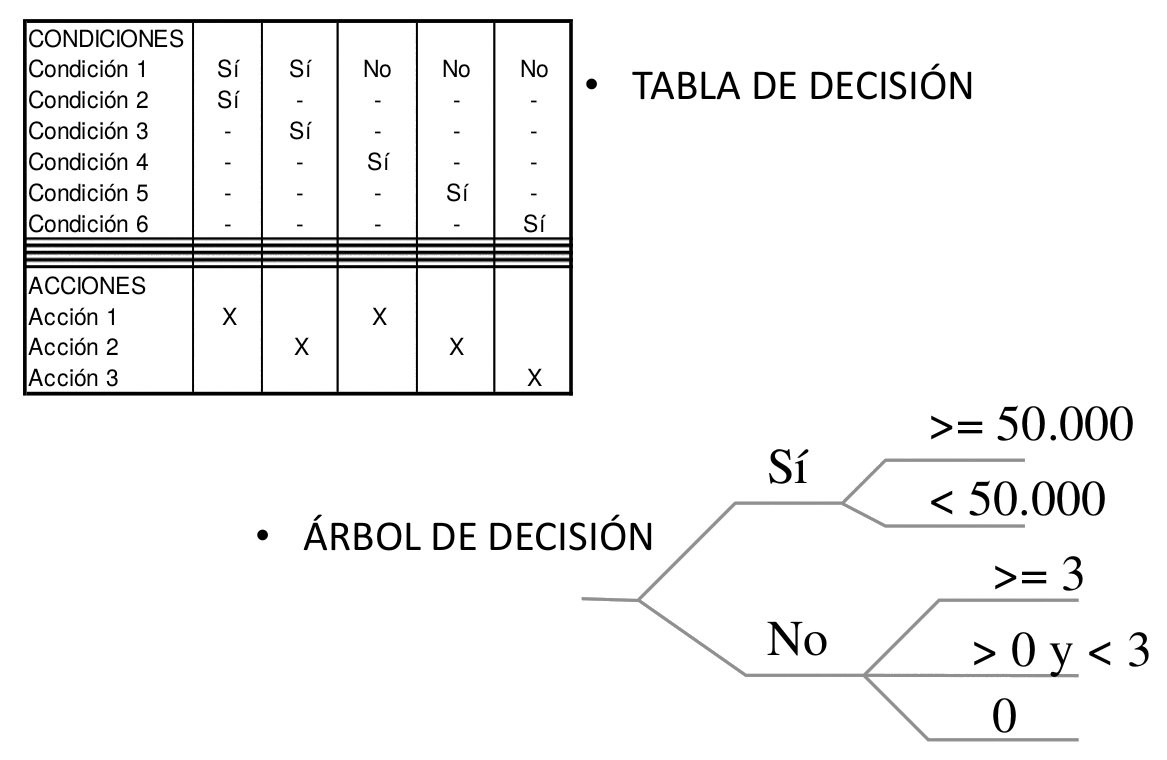
\includegraphics[width=0.6\linewidth]{Resources/Tema5/ejemplosPSPEC.png}
    \caption{Ejemplos de dos PSPEC mediante (1) una tabla de decisión y (2) un árbol de decisión.}
    \label{fig:ejemplosPSPEC}
\end{figure}

\subsection{Estrategia de creación de DFDs y PSPECs}

\begin{enumerate}
    \item \textbf{Diagrama de contexto}:
    \begin{enumerate}
        \item Localizar todas las entidades.
        \item Definir sus flujos con precisión (interfaces).
    \end{enumerate}
    \item \textbf{Diagrama de sistema}:
    \begin{enumerate}
        \item Seleccionar las funciones principales.
        \item Definir los flujos entre dichas funciones; normalmente, a través de almacenes.
        \item Recoger los flujos del diagrama de contexto; normalmente, cada uno entrará en un proceso distinto, y no conviene dividirlos aunque sean flujos múltiples.
    \end{enumerate}
    \item \textbf{Resto de diagramas}:
    \begin{enumerate}
        \item No descomponer al máximo.
        \item Subfunciones principales de cada proceso, e interfaces entre sus procesos resultantes.
        \item Se recogen los interfaces (flujos) de nivel superior y se asignan a alguno de los procesos.
        \item Se pueden desglosar flujos múltiples.
    \end{enumerate}
    \item \textbf{Procesos primitivos}:
    Detenerse cuando:
    \begin{enumerate}
        \item La función puede expresarse en una página.
        \item Los procesos tienen pocos flujos de E/S.
        \item Descomponer implica perder el significado de la función; es decir, se obtienen diagramas demasiado sencillos que complican la compresión global o, dicho de otro modo, que dificultan entender para qué va a servir la función.
    \end{enumerate}
\end{enumerate}


\subsection{Diagramas de flujo de control (DFC, Tiempo--Tiempo)}

Dado que en los DFDs no se representa explícitamente el control o flujo de sucesos del sistema (\uline{cuándo se realizan los procesos o en qué orden}), hay determinados sistemas de software en donde se podrá intuir, pero habrá otros en que \uline{no será posible}. A la hora de \textbf{interpretar el comportamiento de un sistema}, podemos encontrarnos con \textbf{tres situaciones posibles}:

\begin{itemize}
    \item \textbf{Los procesos que figuran en el DFD están activos siempre}. Por ende, no es necesario especificar el control del sistema.
    \item \textbf{Los procesos se activan cuando llegan datos a través de los flujos de entrada}, los transforman y emiten los resultados a través de los flujos de salida, y \textbf{permanecen inactivos hasta la llegada de nuevos datos}. Este comportamiento está implícito en la notación usada.
    \item \textbf{Cada proceso pasa por períodos de actividad e inactividad}, gobernados por \uline{mecanismos más complejos}. Este tipo de situaciones no pueden representarse debidamente en un DFD, por lo que debe crearse un modelo adicional en donde se representen las \uline{señales de control no implícitas en el DFD}.
\end{itemize}

\textbf{Nota:} \textit{El modelo de control del sistema establece el comportamiento de éste a alto nivel, indicando \uline{qué procesos están activos en cada momento o en qué secuencia se realiza la transformación de los datos}. Existe un control de bajo nivel referido a los saltos condicionales y a los bucles, que estaría reflejado en las PSPECs de los procesos.}\\

Para modelar el control del sistema, se emplearán los \textbf{D}iagramas de \textbf{F}lujo de \textbf{C}ontrol (\textbf{DFC}), los cuales consisten en eliminar de los DFDs todo lo relativo a la información de control, y construir una jerarquía de DFCs paralela a la de DFDs. Según esto, se comenzará por el diagrama de contexto, representando en cada par DFD/DFC los mismos procesos y entidades externas, puesto que \uline{representan modelos de la misma parte del sistema con el mismo nivel de detalle, aunque con puntos de vista distintos}.\\

\subsubsection{Elementos}

Las reglas sobre denominación de numeración, relaciones padre--hijo, y balanceo que se aplican a los DFCs \uline{son las mismas} que se establecen para los DFDs.\\

Por otra parte, los elementos que aparecen en un DFC son prácticamente los mismos:

\begin{itemize}
    \item \textbf{Procesos, entidades externas, y almacenes de datos}: Serán los mismos y \uline{tendrán el mismo significado} que en el DFD.
    \item \textbf{Flujos de control}: Se representan mediante trazos discontinuos y modelan el \uline{flujo de información de control en el sistema}. Habrá procesos o entidades externas que generen información de control, y otras que la consuman. Aparte de emplear los flujos entrantes para la activación/desactivación de procesos, un proceso también puede utilizarlos para transformarlos en flujos de salida según la PSPEC correspondiente.
    \item \textbf{Condiciones de datos}: \uline{Flujos de control generados por un proceso del sistema}. Figuran en el DFC y no en el DFD, pero es la PSPEC la que define cómo se calcula su valor a partir de los flujos de entrada del proceso.
    \item \textbf{Almacenes de control}: Se representan igual que los almacenes de datos, pero con trazos discontinuos. Permiten almacenar información de control para ser utilizada posteriormente.
    \item \textbf{Ventanas de especificaciones de control}: Se representan mediante barras, y reciben flujos de control (condiciones de datos junto con flujos de control del exterior), así como los emiten, actuando de este modo como las \uline{transformaciones de flujos de control en el sistema}; dicho de otro modo, dedicen el comportamiento del sistema. Su comportamiento se define en las especificaciones de control (CSPEC). No están etiquetadas, puesto que \uline{todas las ventanas que aparecen en un determinado DFC hace referencia a una única CSPEC} que define cómo se realizan estas transformaciones.
    \item \textbf{Activadores de procesos} Flujos de control especiales que \uline{activan o desactivan procesos} tomando dos posibles valores, \texttt{ON} y \texttt{OFF}. Tienen el mismo nombre que los procesos que controlan, por lo que no suelen representarse en el DFC excepto por fines de claridad. Siguen la jerarquía de los modelos, es decir: un proceso está activo si, y sólo si todos sus antecesores están activos.
\end{itemize}

\begin{figure}[H]
    \centering
    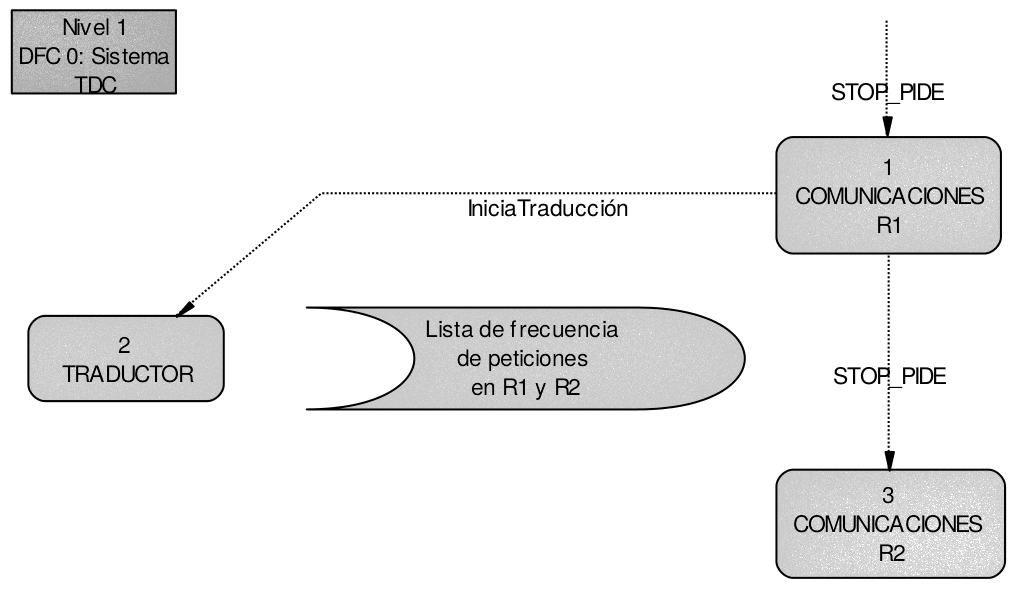
\includegraphics[width=0.8\linewidth]{Resources/Tema5/nivel1_DFC.png}
    \caption{DFC de nivel 1 del TDC.}
\end{figure}

\begin{figure}[H]
    \centering
    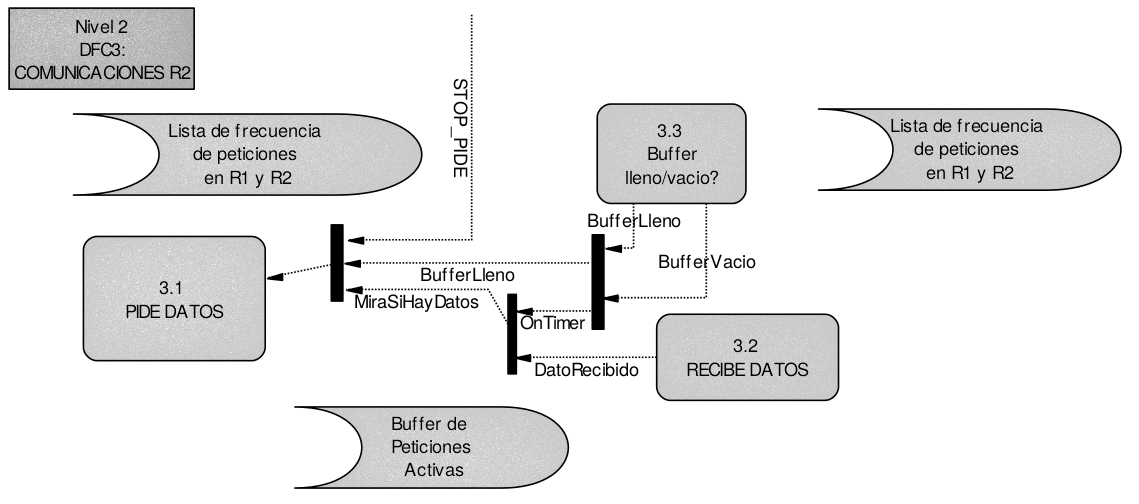
\includegraphics[width=0.9\linewidth]{Resources/Tema5/nivel2_Proceso3_DFC.png}
    \caption{DFC de nivel 2 correspondiente al proceso $3$ del TDC. Nótese la existencia de las condiciones de dato \textit{buffer lleno/buffer vacío}, y del activador entrante en el proceso \textit{3.1 PIDE DATOS}.}
\end{figure}

\textbf{Nota:} \textit{Conviene recordar que, mediante los flujos de control, se define cómo se activan o desactivan los procesos.}\\

\textbf{Nota:} \textit{Dado que los modelos del sistema tienen estructura jerárquica, se considera que un proceso está activo \textbf{solo si todos sus antecesores están activos}. Un proceso que no tiene activador se considera, por lo tanto, activo siempre que sus antecesores lo estén; en caso de tener activador, éste debe tenerse también en cuenta.}\\

\textbf{Nota:} \textit{Los procesos en un DFC indican cómo fluyen los flujos de control a través de ellos. \uline{No representan los estados del sistema} (se encargan los DEs), y \uline{tampoco representan procesamiento ni transformación de los flujos de control} (se encargan las CSPECs).}\\

\textbf{Nota:} \textit{Los DFCs reflejan la información de control que existe en el sistema, y qué procesos y entidades las producen y consumen. Deben ser \uline{combinados} con las CSPECs para reflejar el comportamiento del sistema.}\\

Otro detalle importante es que un flujo de control que entra en un proceso no indica necesariamente que ese proceso se active; la \uline{activación y desactivación de procesos se indica en las CSPECs}. Por lo tanto, un flujo de control entrante puede indicar que:

\begin{itemize}
    \item O bien va a ser utilizado como un dato más para que el proceso lleve a cabo su transformación.
    \item O bien va a ser utilizado para controlar alguno de los procesos en los que se descompone el proceso.
\end{itemize}

\subsubsection{Cómo separar datos y control}

No existen unas normas estrictas para separar, de entre todos los flujos de información, los datos del control. Por norma general, \textbf{se modelarán como señales de control únicamente aquellas que intervengan en la activación y desactivación de algunos de los procesos del sistema de forma no trivial}, mientras que el resto de la información se modelará como datos.\\

En determinadas situaciones, \uline{es posible que un elemento de información determinado se emplee como dato en un proceso y como control en otro}. Para ello, se modelará como dato (trazo continuo) en el DFD, y como control (trazo discontinuo) en el DFC, pero se asignará el mismo nombre a ambos flujos para mostrar que son el mismo.

\subsubsection{Cuándo usar especificaciones de control}

Lo ideal es utilizar DFDs siempre que sea posible, puesto que son más sencillos de realizar y de entender; por ejemplo, el uso de DFCs obligará a mirar en paralelo a los DFDs.\\

En todo caso, debe recordarse siempre que es necesario centrarse en el \textbf{modelo abstracto o lógico} del sistema, mientras que las especificaciones ya tratarán los aspectos de más bajo nivel.

\subsection{Especificaciones de control (CSPEC)}

Son similares a las PSPECs, ya que en ambos casos se definen los detalles procedimentales de cómo se realiza el procesamiento de los flujos de entrada y salida. Sin embargo, hay una diferencia importante entre PSPECs y CSPECs:

\begin{itemize}
    \item Las PSPECs se utilizan para describir las primitivas de proceso.
    \item Las CSPECs sirven para modelar el comportamiento de un DFC, describiendo cómo se procesan los flujos de control. Por lo tanto, habrá, como máximo, una CSPEC por cada DFC de la jerarquía, ya que el primero determina la activación del segundo, utilizando las \textbf{ventanas de control del DFC como interfaces}.
\end{itemize}

Así, se puede concretar que una \textbf{C}ontrol \textbf{SPEC}ification es un documento que \textbf{especifica el comportamiento un DFC} (y, por lo tanto, del sistema). Concretamente, se indica cómo, a partir de las señales de control que entran en una ventana, se determina la activación o desactivación de los procesos comprometidos.\\

Estas CSPECs pueden caracterizarse mediante:

\begin{itemize}
    \item \textbf{Lenguaje estructurado} (pseudocódigo).
    \item \textbf{Sistemas combinacionales} (el valor de salida se determina exclusivamente a partir de los valores de entrada):
    \begin{itemize}
        \item Tablas de decisión: Indican cómo calcular las señales de salida en función de las de entrada.
        \begin{table}[h!]
            \centering
            \resizebox{0.4\textwidth}{!}{%
                \begin{tabular}{|l|c|c|c|c|c|}
                    \hline
                    \multicolumn{6}{|c|}{\textbf{CONDICIONES}} \\ \hline
                    Condición 1 & Sí & Sí & No & No & No       \\
                    Condición 2 & Sí & -  & -  & -  & -        \\
                    Condición 3 & -  & Sí & -  & -  & -        \\
                    Condición 4 & -  & -  & Sí & -  & -        \\
                                &    &    &    &    &          \\ \hline
                    \multicolumn{6}{|c|}{\textbf{ACCIONES}}    \\ \hline
                    Acción 1    & X  &    & X  &    &          \\
                    Acción 2    &    & X  &    & X  & X        \\\hline
                \end{tabular}
            }
            \caption{Ejemplo de tabla de decisiones de un proceso.}
        \end{table}
        \item Tablas de activación de procesos: Similares a las anteriores, pero indicando para cada proceso del DFC si está activo o no ante cada combinación.
    \end{itemize}
    \item \textbf{Sistemas secuenciales}:
    \begin{itemize}
        \item Diagramas de Estados: Autómatas finitos.
        \begin{figure}[h!]
            \centering
            \includegraphics[width=0.9\linewidth]{Resources/estados}
            \caption{Ejemplo de un diagrama de estados.}
        \end{figure}
        \item Redes de Petri: Técnica muy apropiada en el caso de tratar con sistemas de comportamiento asíncrono concurrente.
        \begin{figure}[H]
            \centering
            \includegraphics[width=0.75\linewidth]{Resources/redPetri}
            \caption{Proceso de generación de una reclamación modelado en redes de Petri.}
        \end{figure}
    \end{itemize}
\end{itemize}

\subsection{Estrategia de creación de DFCs y CSPECs}

\begin{enumerate}
    \item Construir una jerarquía de DFCs paralela a la de DFDs.
    \item Cada par DFC/DFD representa los mismos procesos y las mismas entidades externas.
    \item Solo se introducen las señales de control que no estén implícitas en el DFD.
    \item Cada DFC se desarrolla en un CSPEC.
\end{enumerate}

\begin{figure}[H]
    \centering
    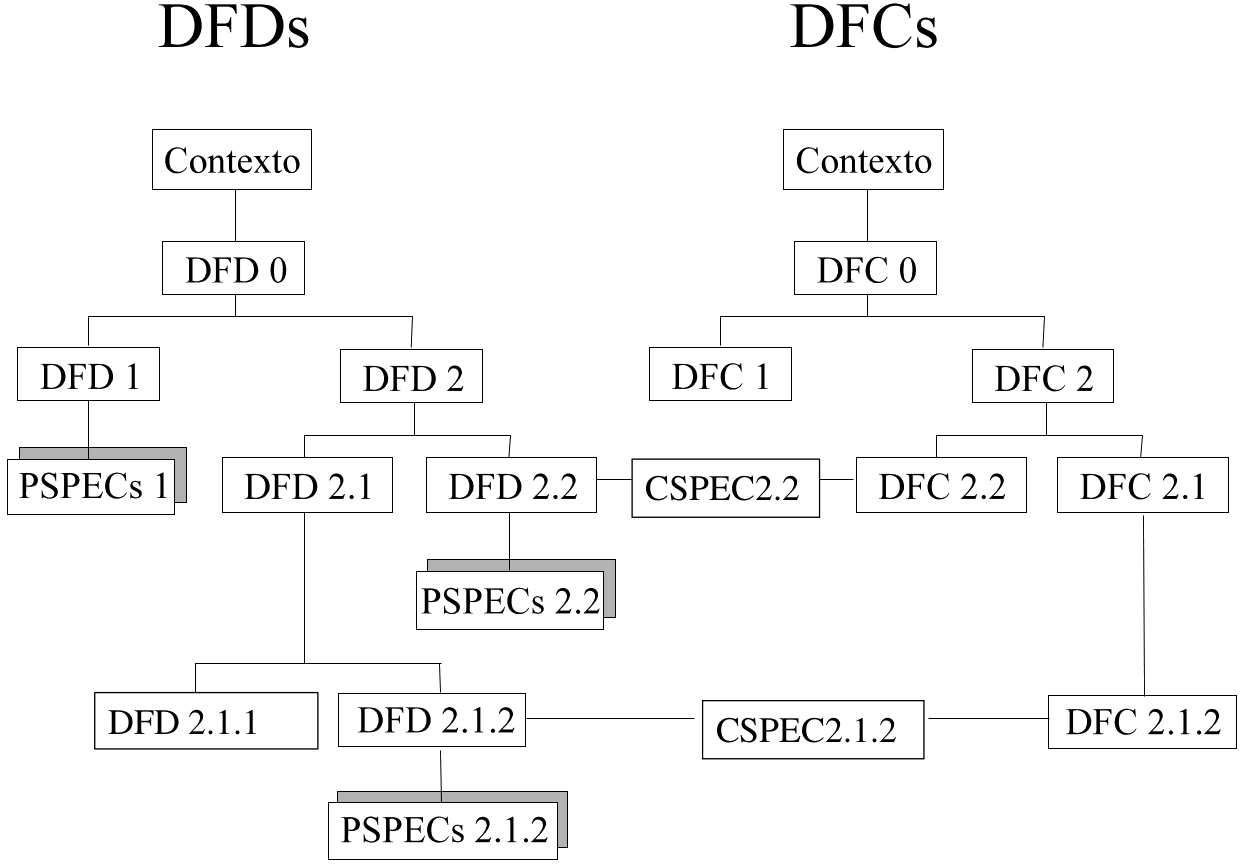
\includegraphics[width=0.8\linewidth]{Resources/Tema5/jerarquiaDFCs.png}
    \caption{Ejemplificación de la jerarquía de DFCs paralela a la de DFDs.}
\end{figure}

En resumen, por cada DFD se crea un DFC gemelo si alguno de los procesos del DFD genera o consume información de control. Además, si alguno de los procesos del DFD es activado o desactivado de forma no implícita, éste DFC llevará una ventana de control y se hará una CSPEC para indicar cuándo se realiza la activación y desactivación.

\subsection{Diagramas Entidad--Relación (DER)}

Los \textbf{D}iagramas \textbf{E}ntidad--\textbf{R}elación resuelven las insuficiencias que se pueden producir en la representación de datos complejos mediante los almacenes en los diagramas de flujo de datos (DFD). Para ello, no solo se muestra la información contenida, sino también las relaciones que existen entre los propios datos.

\begin{figure}[H]
    \centering
    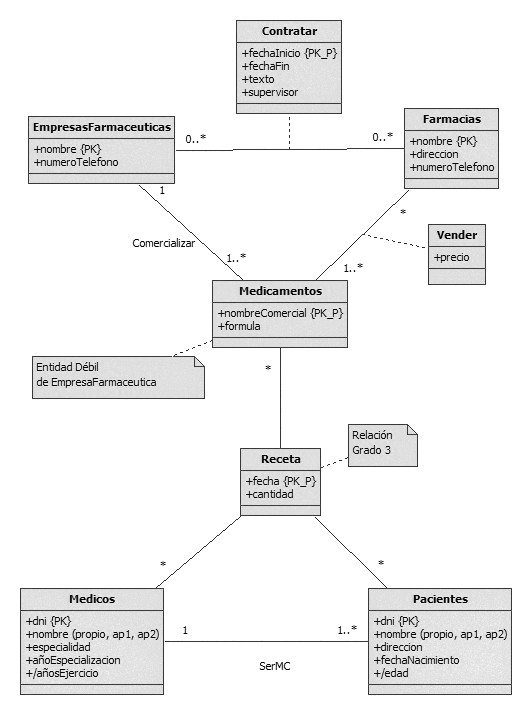
\includegraphics[width=0.6\linewidth]{Resources/Tema5/Caso12_RecetasRayosX_MER.jpg}
    \caption{Ejemplificación de un Diagrama Entidad--Relación.}
\end{figure}

\subsection{Comprobaciones}

Una vez esté realizada la especificación estructurada, debe comprobarse si cumple las siguientes propiedades:

\begin{enumerate}
    \item \textbf{Compleción}: Los modelos son completos.
    \item \textbf{Integridad}: No existen contradicciones ni incoherencias entre los modelos.
    \item \textbf{Exactitud}: Los modelos cumplen los requisitos del usuario.
    \item \textbf{Calidad}: Presencia de estilo, legibilidad y facilidad de mantenimiento.
\end{enumerate}

\textbf{Nota:} \textit{Es recomendable realizar las comprobaciones elaborando una checklist en la que se comprueben, con profundidad, aspectos sobre todas estas propiedades.}

\subsection{Consistencia entre modelos}

El conjunto de modelos tiene como misión dar una visión global del sistema, desde diversos puntos de vista; por lo tanto, representan siempre el mismo sistema, así que deben ser consistentes.\\

Las técnicas matriciales se utilizan \textbf{principalmente para ayudar a verificar la consistencia entre los componentes de distintos modelos} de un sistema, ya sean centrados en la dimensión de las funciones, en la de la información, o en la temporal.

\begin{enumerate}
    \item \textbf{Matriz Entidad/Función}: Visualiza las relaciones existentes entre las funciones que lleva a cabo un sistema y la información necesaria para soportarlas.\\
    
    Los elementos de las filas son entidades o relaciones presentes en el DER, mientras que los de las columnas pueden ser funciones de alto nivel representadas en un DFD.\\

    En cada celda se incluyen las \textbf{acciones} que puede realizar la función (\textbf{I}nsertar, \textbf{L}eer, \textbf{M}odificar y \textbf{B}orrar).

    \begin{table}[h!]
        \centering
        \begin{tabular}{cl|c|c|c|} \cline{3-5}
                                                                                                    &                                   & \multicolumn{3}{c|}{\textbf{Funciones}}                              \\ \cline{3-5}
                                                                                                    &                                   & Gestionar Presupuesto                   & Gestionar Cliente & \ldots \\ \cline{2-5}
            \parbox[t]{2mm}{\multirow{3}{*}{\rotatebox[origin=c]{90}{{\small \textbf{Entidades}}}}} & \multicolumn{1}{|c|}{Cliente}     & L                                       & I, M, B           &        \\ \cline{2-5}
                                                                                                    & \multicolumn{1}{|c|}{Presupuesto} & I, M, B                                 &                   &        \\ \cline{2-5}
                                                                                                    & \multicolumn{1}{|c|}{\ldots}      &                                         &                   &        \\ \cline{2-5}
        \end{tabular}
        \caption{Ejemplo de Matriz Entidad/Función.}
        \label{tab:matrizEF}
    \end{table}

    \item \textbf{Matriz Entidad/Entidad}: Muestra las relaciones habituales del DER, indicando en cada celda la relación entre las entidades implicadas. Es de utilidad, sobre todo, cuando se presenta un número alto de entidades.
          
          \begin{table}[h!]
              \centering
              \begin{tabular}{cl|c|c|c|} \cline{3-5}
                                                                                                          &                                   & \multicolumn{3}{c|}{\textbf{Entidades}}                        \\ \cline{3-5}
                                                                                                          &                                   & Cliente                                 & Presupuesto & \ldots \\ \cline{2-5}
                  \parbox[t]{2mm}{\multirow{3}{*}{\rotatebox[origin=c]{90}{{\small \textbf{Entidades}}}}} & \multicolumn{1}{|c|}{Cliente}     &                                         & Tiene       &        \\ \cline{2-5}
                                                                                                          & \multicolumn{1}{|c|}{Presupuesto} &                                         &             &        \\ \cline{2-5}
                                                                                                          & \multicolumn{1}{|c|}{\ldots}      &                                         &             &        \\ \cline{2-5}
              \end{tabular}
              \caption{Ejemplo de Matriz Entidad/Entidad.}
              \label{tab:matrizEE}
          \end{table}

          %mecago en dios tanto royo para definir señales de control y ahora usa eventos....
    \item \textbf{Matriz Evento/Entidad} (evento $\equiv$ señal de control): Muestra las acciones que provocan los eventos sobre las entidades (datos almacenados): (\textbf{I}nsertar, \textbf{L}eer, \textbf{M}odificar y \textbf{B}orrar).

        \begin{table}[h!]
              \centering
              \begin{tabular}{cl|c|c|c|} \cline{3-5}
                                                                                                        &                                             & \multicolumn{3}{c|}{\textbf{Entidades}}                        \\ \cline{3-5}
                                                                                                        &                                             & Cliente                                 & Presupuesto & \ldots \\ \cline{2-5}
                  \parbox[t]{2mm}{\multirow{3}{*}{\rotatebox[origin=c]{90}{{\small \textbf{Eventos}}}}} & \multicolumn{1}{|c|}{Datos del cliente}     & I, M, B                                 &             &        \\ \cline{2-5}
                                                                                                        & \multicolumn{1}{|c|}{Datos del presupuesto} & I                                       & I, M, B     &        \\ \cline{2-5}
                                                                                                        & \multicolumn{1}{|c|}{\ldots}                &                                         &             &        \\ \cline{2-5}
              \end{tabular}
              \caption{Ejemplo de Matriz Evento/Entidad.}
              \label{tab:matrizEvE}
          \end{table}
\end{enumerate}


\section{Metodología del análisis estructurado}

Una vez vistas todas las anteriores notaciones, se verá ahora cómo coordinarlas durante el trabajo.

\subsection{Fases}

\subsubsection{Creación del modelo de procesos}

El punto de partida será la creación del modelo de procesos del sistema, modelando el ámbito de información y el funcional mediante DFDs y PSPECs.\\

Inicialmente, debe \textbf{revisarse toda la documentación inicial}; es importante pensar antes de ponerse a dibujar diagramas. Por ejemplo, puede realizarse un \textbf{análisis gramatical} de toda esta información, para facilitar la identificación de muchos de los componentes del sistema:

\begin{itemize}
    \item Las entidades externas se corresponderían con los nombres.
    \item Los flujos y almacenes de datos también se corresponderían con los nombres.
    \item Los procesos se corresponderían con los verbos.
\end{itemize}

Además, la especificación (documentación) estudiada también establecerá las relaciones entre dichos nombres y verbos de por sí. A pesar de que lo obtenido hasta el momento no sea completamente correcto, o esté incompleto, sí marca un buen punto de partida.\\

Tras ello, se comienza a realizar el \textbf{DFD de contexto}, y se va refinando en mayores niveles de detalle siguiendo las \textbf{reglas de construcción}. Es importante respetar las reglas de \textbf{acoplamiento mínimo} entre procesos distintos, y de \textbf{máxima cohesión} dentro de un proceso, así como mantener la \textbf{consistencia} entre los diferentes componentes de la jerarquía de DFDs. También debe recordarse el \textbf{evitar detalles de implementación}, así como \textbf{ir incluyendo en el diccionario de datos (DD) los elementos de los DFDs}.\\

El proceso de descomposición finalizará una vez de \textbf{encuentren los procesos primitivos} (procesos sencillos con máxima cohesión $\equiv$ realizan una única función), y que se describirán mediante \textbf{PSPECs}. Estos últimos no contienen definiciones de datos, por lo que no pueden actuar como almacenes de datos, sino emplear tan solo variables locales, aparte de los datos de entrada.

\subsubsection{Creación del modelo de control}

\textbf{No todos los sistemas requieren modelos de control}, al poder estar esta información presente, a veces, de forma implícita en los DFDs. En caso de realizarse, hay que tener \textbf{especial cuidado en no caer en detalles de implementación}.\\

Esta actividad debe comenzar por \textbf{establecer una jerarquía de DFCs simétrica a la de DFDs}, de modo que cada par DFD/DFC contiene los mismos procesos, almacenes de datos, y entidades externas, y hasta en la misma posición, para facilitar la identificaciónde estos elementos. A continuación, se \textbf{eliminan del DFD todos los flujos que transporten información de control}, y se representarán en los DFCs.\\

A \textbf{cada par DFD/DFC} en donde el DFD es antecesor inmediato de procesos primitivos, \textbf{le podrá corresponder una CSPEC}; esta puede ser combinacional, secuencial o compuesta, y se escogerá siempre el modelo más sencillo posible. Es importante recordar que debe \textbf{mantenerse la consistencia de flujos entre las ventanas de control y las CSPECs}.

\subsubsection{Creación del modelo de datos}

\textbf{Si los datos que maneja el sistema tienen una estructura compleja}, no bastará con definir en el DD el contenido de cada uno. Se desarrollará en su lugar un modelo de datos empleando \textbf{DERs}, donde se muestren las \textbf{relaciones} que existan entre los datos que maneje el sistema.

\subsubsection{Consistencia entre modelos}

Finalmente, una vez realizados los distintos modelos del sistema, deberían llevarse a cabo todas las \textbf{técnicas de consistencia entre modelos} que se consideren necesarias.


\section{Modelos del sistema}

\subsection{El modelo esencial}

El \uline{modelo esencial} del sistema (algunas veces llamado modelo lógico) representa lo que \textbf{el sistema debe hacer para satisfacer los requisitos del usuario}. Es, por lo tanto, un modelo abstracto que supone que disponemos de una \uline{tecnología perfecta} sin coste alguno.\\

Este modelo es el \textbf{resultado de la fase de análisis de requisitos del sistema}, por lo que debe estar completamente libre de detalles de implementación. Algunos errores típicos al realizarlo son:

\begin{itemize}
    \item \textbf{Secuenciar los procesos del DFD}: Deben ser lo más concurrentes posibles, en lugar de pensar que el sistema realiza las tareas una detrás de otra. El único secuenciamiento que debe aparecer en los DFDs es por la dependencia de datos; cualquier otra secuencia es puramente arbitraria, y dependerá fundamentalmente de necesidades de implementación.
    \item \textbf{Utilizar ficheros temporales o de backup}: Estos se usan para conectar procesos que no pueden ejecutarse simultáneamente por limitaciones de la capacidad del hardware, y no porque deban ejecutarse de forma secuencial. Pero, en este modelo esencial, estamos suponiendo que contamos con una tecnología perfecta con la que evitar este tipo de limitaciones, por lo que no se requiere esta clase de ficheros.
    \item \textbf{Utilizar información redundante o que puede ser derivada}: En el modelo esencial no se usará nunca este tipo de información, ya que tiene más que ver con la eficiencia de implementación que con los requisitos del modelo. \textit{Por ejemplo, un error sería almacenar en una base de datos un dato que podría declararse como derivado, solo por evitar calcularlo cada vez que se requiera}.
\end{itemize}

A partir del modelo esencial, los diseñadores podrán decidir cómo implementar el sistema, usando la \uline{tecnología disponible}.

\subsection{Modelo de implementación}

Sin embargo, lo normal es que el cliente proporcione más información que los requisitos del sistema, y que decida también sobre detalles de implementación: qué funciones serán manuales y cuáles automáticas, el formato de los datos de salida, etc. Toda esta información no se refiere a los requisitos esenciales del sistema, sino a los \uline{requisitos de implementación}, que formarán parte del \uline{modelo de implementación} del sistema.\\

El desarrollo de este modelo es una tarea que está a \textbf{medio camino entre el análisis y el diseño}. No puede ser desarrollado solo por el analista y el cliente, dado que se necesita el consejo de diseñadores e implementadores, ya que conocen la tecnología disponible. Por otra parte, no puede ser realizado únicamente por diseñadores e implementadores, porque el usuario debe definir una gran cantidad de requisitos de información, y es el analista quien los describe, haciendo de vínculo entre el cliente y el equipo de desarrollo.\\

En definitiva, este modelo será una \textbf{versión revisada y anotada del modelo esencial, especificando todos esos detalles adicionales}. Sobre ellos, se puede destacar:

\begin{itemize}
    \item La elección de dispositivos de entrada y salida.
    \item La elección de los dispositivos de almacenamiento.
    \item El formato de las entradas y las salidas.
    \item La secuencia de operaciones de entrada y salida, incluyendo la definición de cómo será el diálogo con el usuario.
    \item El volumen de datos esperado.
    \item El tiempo de respuesta requerido.
    \item La realización de copias de seguridad, y las posibilidades de exportar bajo demanda datos contenidos en el sistema.
    \item La seguridad.
\end{itemize}

\newpage
\part{Pruebas del software}

\section{Introducción}

Una de las características típicas de los ciclos de vida en el desarrollo de software es la realización de controles periódicos, con el objetivo de evaluar la calidad de los productos generados, y poder \textbf{detectar así fallos en ellos cuanto antes}. Aún así, todo sistema/aplicación debe ser \textbf{probado}, independientemente de estas revisiones, mediante su \textbf{ejecución controlada antes de ser entregado al cliente}; estas se denominan habitualmente como \uline{pruebas}.\\

Las pruebas permiten verificar y validar el software; cabe recordar el significado de estos dos términos:

\begin{itemize}
    \item \textbf{Verificación} (pruebas de \uline{caja blanca}): Proceso de evaluación de un sistema o de uno de sus componentes para determinar si los productos de la fase en la que se realizan estas pruebas satisfacen las condiciones impuestas al principio de dicha fase. Dicho de otro modo, se puede decir que se pregunta \uline{si se está construyendo correctamente el producto}.
    
    \item \textbf{Validación} (pruebas de \uline{caja negra}): Proceso de evaluación del sistema o de uno de sus componentes para determinar, bien sea durante o al final del desarrollo, si satisface los requisitos especificados. Dicho de otro modo, se puede decir que se pregunta \uline{si se está construyendo el producto correcto}.
\end{itemize}

Como se puede ver, el contar con la posibilidad de enfocar las pruebas hacia cualquiera de estos dos puntos de vista permite enfrentar cualquier fase del ciclo de vida a:

\begin{itemize}
    \item \textbf{La metodología de la propia fase}: Verificación.
    \item \textbf{Los requisitos}: Validación.
\end{itemize}

\section{Definiciones}

El \textit{IEEE} propone, entre otras, las siguientes definiciones en relación a las pruebas.

\paragraph{Prueba} Actividad en la que un sistema o uno de sus componentes se ejecuta en circunstancias previamente especificadas, y cuyos resultados son observados, registrados y evaluados comprobando algún aspecto determinado de antemano. \textit{Procedimiento de ejecutar un programa con el fin de encontrar errores.}\\

Una prueba consta de uno o más casos de prueba.

\paragraph{Caso de prueba} Conjunto de entradas, condiciones de ejecución y resultados esperados desarrollados para un objetivo particular. \textit{Por ejemplo: ejercitar un camino concreto de un programa, o verificar el cumplimiento de un determinado requisito.}\\

Por extensión, un caso de prueba válido debe comprobar que se deja hacer lo que se debería, y que no se permite hacer lo que no. Además, un buen caso de prueba es aquel que tiene una \uline{alta probabilidad de detectar un error}.\\

\textbf{Nota:} \textit{Por ejemplo, una prueba del módulo de menús de un software para comedores constaría de varios casos de prueba; estos podrían ser que un jefe de una cafetería pueda \{insertar, borrar, modificar\} un menú.}

\paragraph{Defecto} Incorrección en el software que \textbf{genera un fallo}. \textit{Por ejemplo: un proceso, una definición de datos o un paso de procesamiento incorrectos en un programa.}

\paragraph{Fallo} Incapacidad de un sistema o de alguno de sus componentes para realizar las funciones requeridas dentro de los requisitos de rendimiento especificados. \textit{Es el hecho de que el software no pueda funcionar.}\\

\textbf{Nota:} \textit{Un fallo causado por un defecto es culpa de los desarrolladores, mientras que un fallo sin defecto es culpa del entorno, al poder presentar características como ser altamente cambiante. Por este motivo, es importante concretar un entorno para las pruebas, así como replicar las condiciones en las que el software será explotado.}

\paragraph{Error} Presenta varias acepciones:
\begin{itemize}
    \item Diferencia entre un valor calculado, observado o medido, y el valor verdadero, especificado o teóricamente correcto.
    \item Resultado incorrecto.
    \item Defecto en el software.
    \item \uline{Acción humana que conduce a un resultado incorrecto}.
\end{itemize}

\begin{figure}[H]
    \centering
    \includegraphics[width=0.8\linewidth]{Resources/cuernos}
    \caption{Recuerda: error, defecto y fallo no son lo mismo. Al final, se provocan efectos negativos.}
    \label{fig:cuernos}
\end{figure}


\section{Filosofía de las pruebas del software}

Las características especiales del software, como que carezca de leyes que rijan su comportamiento, o presentar una gran complejidad habitualmente, hacen aún más difícil la tarea de probarlo, de modo que la \textbf{prueba exhaustiva del software es impracticable}: \uline{\textbf{no} se pueden probar todas las posibilidades incluso en programas pequeños y sencillos}. Además, esta situación se ve empeorada por la presencia de prejuicios (estimaciones subjetivas por parte de los trabajadores sobre lo bien que han realizado su trabajo), y por la habitual falta de tiempo en el desarollo del proyecto. Por ello, es interesante estudiar cuál es la mejor actitud a seguir en esta actividad; en general, será interesante \uline{sistematizar todo lo posible} de las pruebas, para ahorrar en tiempo y recursos.\\

Es necesario, en primer lugar, un fuerte cambio de mentalidad, dejando atrás la visión constructiva del desarrollo del software, para dar paso a la \uline{visión destructiva} de intentar tirar abajo lo construido. Al final el objetivo de las pruebas, desde el punto de vista del proyecto, es la detección de defectos en el software, por lo que \textbf{el descubrir un defecto debe considerarse como el éxito de una prueba}.\\

En segundo lugar, también es necesario tener presente que todo el mundo comete errores, por lo que no hay que sentirse culpable por haber encontrado una metedura de pata; desde luego, es mejor que el desarrollador se encuentre con un fallo, en lugar de que tenga que ser reportado por el cliente. Es más, los defectos no son siempre el resultado de la negligencia, sino que influyen múltiples factores en su aparición, como la mala comunicación entre los miembros del equipo, que pueden dar lugar a malentendidos.\\

Además del objetivo mencionado anteriormente, también cabe destacar que el objetivo de las pruebas, pero ahora desde el punto de vista de ser un proceso, es el \textbf{diseñar técnicas que permitan un desarollo sistemático de pruebas} para garantizar ese primer objetivo; es en esta visión en la que se centrará este documento.\\

Finalmente, la realización de pruebas en el software también cuenta con determinadas ventajas secundarias:

\begin{itemize}
    \item \textbf{Demuestran hasta qué punto se verifican los requisitos:} No siempre va a ser posible satisfacer todos; por ejemplo, es posible que queden en ``segundo plano'' los requisitos estimulantes (quedarían bien), o incluso podrían verse afectados requisitos más relevantes por limitaciones de tiempo y de recursos, agravados aún más en el caso de que se produzcan cambios en los requisitos durante el desarrollo del proyecto.
    \item \textbf{Se generan datos de prueba que informan sobre la fiabilidad del software.}
\end{itemize}

\textbf{Nota:} \textit{La realización de pruebas no asegura la ausencia de fallos; pero, el descubrimiento de un defecto, significa un éxito para la mejora de la calidad.}\\

\textbf{Nota:} \textit{A veces, no será posible subsanar todos los errores encontrados por limitaciones de tiempo y de recursos. En estos casos, es necesario discernir entre qué errores se corregirán y cuáles no; por ejemplo, no se corregirán aquellos que fallen en menos del 10\% de los tests.}

\subsection{Principios}

Los seis primeros fueron enunciados por \textit{Davis}, y los restantes por \textit{Myers}; a estos últimos, es además necesario incluir de nuevo los principios 3 y 6.

\begin{enumerate}
    \item \textbf{A todas las pruebas se les debería poder hacer un seguimiento hasta los requisitos del cliente}. Se logra mediante la \uline{trazabilidad}:
    \begin{itemize}
        \item \textbf{Trazabilidad hacia arriba}: Si se detecta un fallo, es posible identificar a qué requisitos afecta para evaluar si compensa o no solventarlo.
        \item \textbf{Trazabilidad hacia abajo}: Si se produce un cambio en un requisito, es posible determinar qué pruebas es necesario cambiar para poder validar este nuevo requisito.
    \end{itemize}
    \item \textbf{Las pruebas deberían planificarse mucho antes de que empiecen, y ser repetibles} (probar $\rightarrow$ corregir, probar $\rightarrow$ corregir\ldots): La planificación de pruebas puede comenzar tan pronto como esté completo el modelo de requisitos. La definición detallada de los casos de prueba puede empezar tan pronto como el modelo de diseño se haya consolidado. Como se puede ver, es posible planificar y diseñar algunas pruebas incluso antes de generar ningún código.
    \item \textbf{El 80\% de los errores surgen al hacer el seguimiento del 20\% de los módulos del software (\textit{Principio de Pareto})}: Conviene aislar los módulos sospechosos.
    \item \textbf{Las pruebas tendrían que hacerse de lo pequeño hacia lo grande}: En caso contrario, será difícil concretar el origen de los problemas.
    \item \textbf{No son posibles pruebas exhaustivas, ni probar todo al mismo tiempo}: Sin embargo, es posible cubrir adecuadamente la lógica del programa y asegurarse de que se han aplicado todas las condiciones en el diseño a nivel de componente.
    \item \textbf{Las pruebas deberían ser realizadas por un equipo independiente del de desarrollo}: El haber sido el responsable de la construcción del software probablemente lleve a realizar pruebas menos rigurosas, así como es habitual que condiciones que se olvidaron al crear el programa vuelvan a ser obviadas al escribir casos de prueba. \textit{Por ejemplo: que se reciba un fichero vacío}.\\
    

    \item \textbf{Cada caso de prueba debe definir el resultado de salida esperado} y compararlo con el realmente obtenido.
    \item \textbf{Se debe inspeccionar a conciencia el resultado de cada prueba}, para así poder descubrir posibles síntomas de defectos.
    \item \textbf{Al generar casos de prueba se deben incluir tanto datos de entrada válidos y esperados, como no válidos e inesperados.}
    \item \textbf{Las pruebas deben centrarse en probar si el software}:
          \begin{itemize}
              \item \textbf{No hace lo que debe hacer}.
              \item \textbf{Hace lo que no debe hacer}.
          \end{itemize}
    \item \textbf{Se deben evitar los casos desechables}; es decir, los no documentados o diseñados sin cuidado: Como suele ser necesario probar una y otra vez el software, el no documentar o no guardar los casos significa repetir constantemente el diseño de casos de prueba. \textit{Por ejemplo: se incluirían aquí las pruebas tecleadas sobre la marcha.}
    \item \textbf{No deben hacerse casos de prueba suponiendo que no hay defectos en los programas}: Dicho de otro modo, no deben dedicarse pocos recursos a las pruebas.
    \item \textbf{Las pruebas son una tarea tanto o más creativa que el desarrollo de software}: Dado que no existen técnicas rutinarias para concebirlas.
\end{enumerate}

Una vez visto todo esto, se puede concluir que la filosofía más adecuada consiste en planificar y diseñar las pruebas de forma sistemática para poder detectar el máximo número y variedad de defectos con el mínimo consumo de tiempo y esfuerzo. Es también necesario recordar que un buen caso de prueba es aquel que tiene una gran probabilidad de encontrar un defecto no descubierto aún, y que el éxito de una prueba consiste en detectar un defecto no encontrado antes.


\section{El proceso de prueba}

En la siguiente figura, se puede ver una representación del proceso completo relacionado con las pruebas basada, en parte en el estándar, y en parte en \textit{Pressman}. En este documento, no se hará más énfasis en él.

\begin{figure}[H]
    \centering
    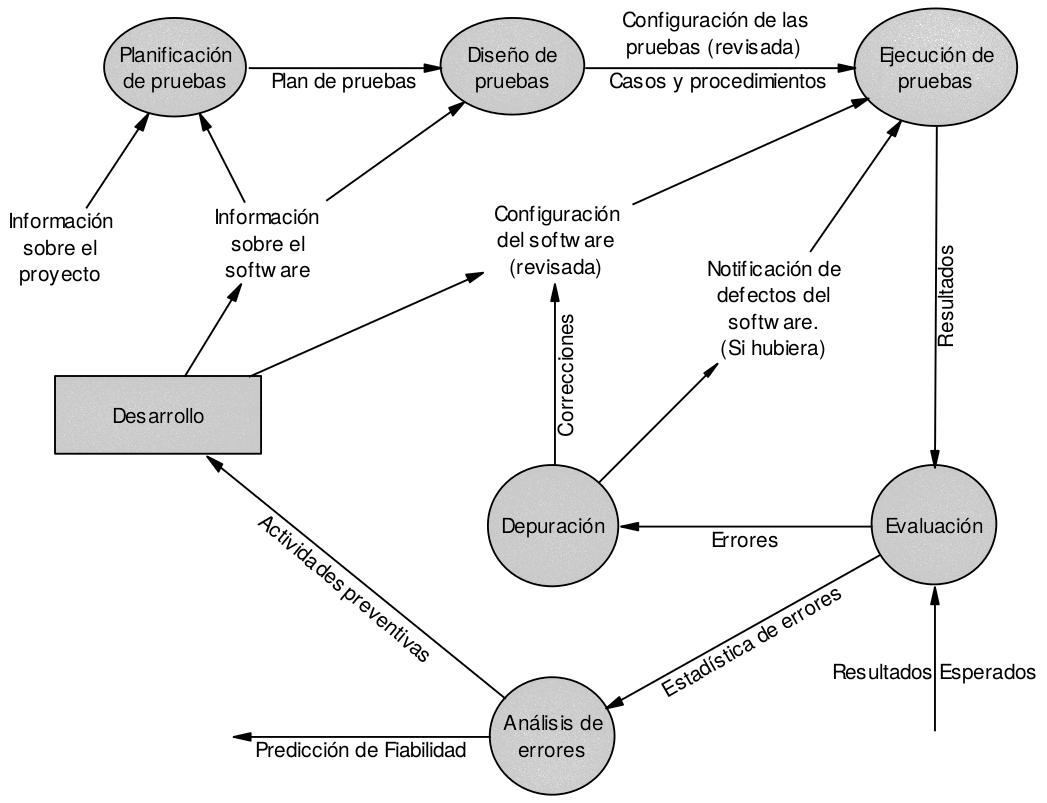
\includegraphics[width=0.8\linewidth]{Resources/Tema6/ProcesoPruebas_IEEE_Pressman.png}
    \caption{Proceso relacionado con las pruebas según el estándar y según \textit{Pressman}. Las flechas entrantes en cada actividad representan información de entrada requerida para su realización.}
\end{figure}


\section{Técnicas de diseño de casos de prueba}

Como se comentó anteriormente, el diseño de casos de prueba está totalmente condicionado por la imposibilidad de probar exhaustivamente el software. Por ello, las técnicas de diseño de casos de prueba tienen como objetivo \textbf{conseguir una confianza aceptable en la que se detectarán los defectos existentes}, al no ser obtenible la seguridad total, \textbf{sin consumir una cantidad excesiva de recursos}. Alcanzar un equilibrio entre dicha confianza y el uso de recursos no es sencillo cuanto menos.\\

La idea fundamental para el diseño de casos de prueba es \textbf{elegir algunos de ellos que, por sus características, se consideren representativos del resto}; de este modo, se asume que, si no se detectan defectos en el software al ejecutar dichos casos, se puede contar con un cierto nivel de confianza en que el programa no tiene defectos. Es necesario recurrir a ciertos criterios de elección para construir los mejores casos de prueba posibles, como preguntarse cómo puede fallar el software, escoger casos no redundantes, que no sean ni demasiado sencillos ni demasiado complejos\ldots\\

Existen dos enfoques principales:

\begin{enumerate}
    \item \textbf{Estructural o de caja blanca} (verificación): Consiste en \uline{centrarse en la estructura interna (implementación)} del programa, realizando pruebas que aseguren que todos los módulos o \uline{componentes internos funcionan bien y encajan correctamente}. \textit{La prueba exhaustiva consistiría en probar todos los posibles caminos de ejecución.}
    \item \textbf{Funcional o de caja negra} (validación): Consiste en \uline{estudiar la especificación de las funciones (interfaz)}, \uline{dejando de importar cómo está implementada la aplicación}. De esta especificación, se derivan los casos, probándose que cada función es completamente operativa puesto que se conoce qué es lo que debe realizar. \textit{La prueba exhaustiva consistiría en probar todas las posibles entradas y salidas del programa.}
\end{enumerate}

Cabe destacar que estos enfoques no son excluyentes, sino que \textbf{son complementarios}. Por ejemplo, podrían diseñarse inicialmente los casos de prueba de caja negra y, a la hora de diseñar los de caja blanca, cabría la posibilidad de que algunos casos de estos últimos ya estuviesen cubiertos; al final, es necesario que se recorran determinados caminos en la ejecución de las pruebas de caja negra.


\section{Pruebas estructurales (de caja blanca)}

Es interesante realizar pruebas de caja blanca porque:

\begin{itemize}
    \item Los errores tipográficos son aleatorios, por lo que pueden aparecer en cualquier parte del programa, se ejecute regularmente o no.
    \item Se suele creer que un determinado flujo es poco probable cuando, de hecho, puede ejecutarse regularmente.
    \item En relación al anterior punto, en general, la probabilidad e importancia de un trozo de código suelen ser calculadas de forma muy subjetiva. \textit{Por ejemplo: si el programador sabe que un camino normalmente se ejecutará poco, es probable que le preste menos atención que a otros, incrementándose por lo tanto la probabilidad de que se encuentren errores en él.}
\end{itemize}

El diseño de casos de prueba tiene que basarse en la \textbf{elección de caminos importantes que ofrezcan una seguridad aceptable de descubrir un defecto}, y para ello se utilizan los criterios de cobertura lógica. No requieren el uso de representaciones gráficas, pero se suelen utilizar grafos de flujo (estrechamente relacionados con los diagramas de flujo de control), con el objetivo de \uline{convertir el código en un grafo y facilitar así la visualización de sus posibles caminos}.

\begin{figure}[H]
    \centering
    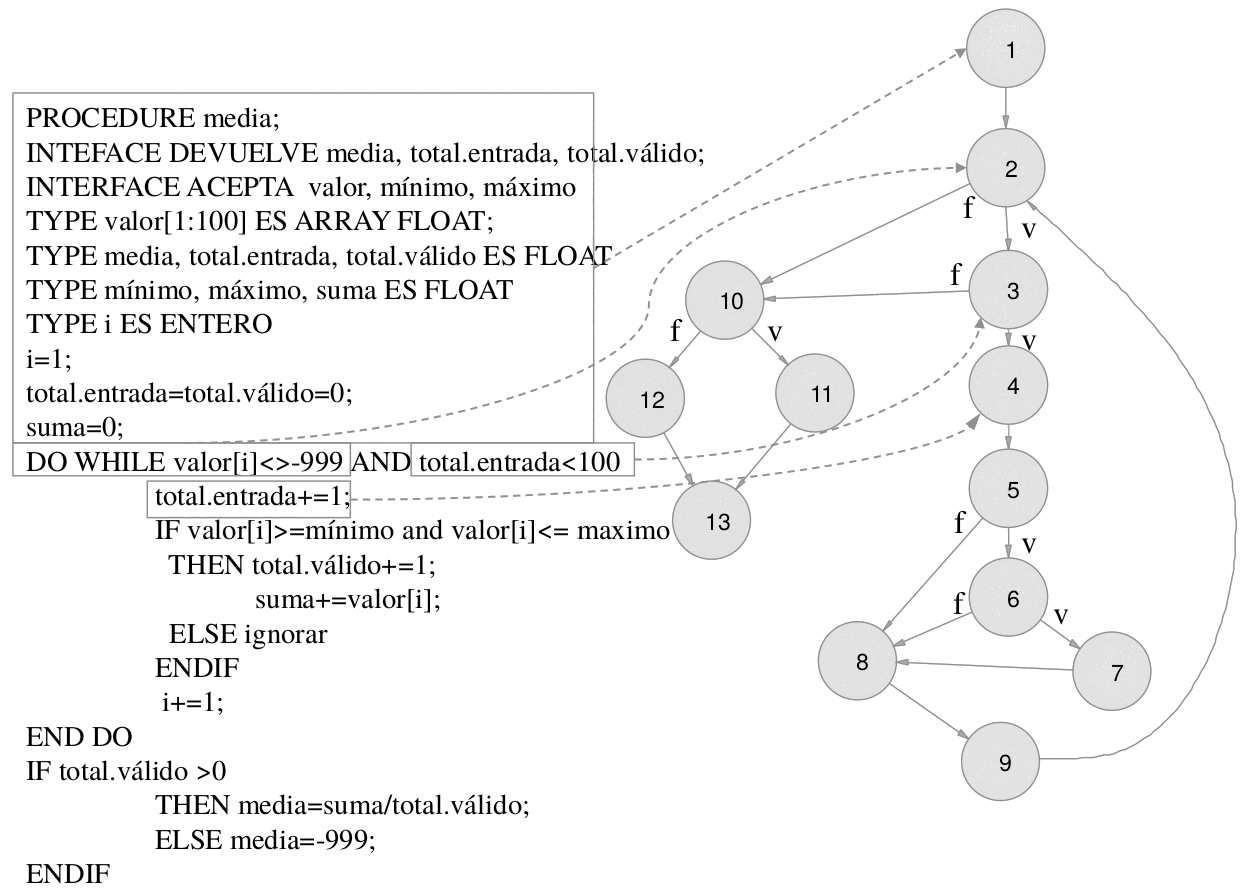
\includegraphics[width=0.8\linewidth]{Resources/Tema6/Ejemplo_GrafoFlujo.png}
    \caption{Ejemplo de un grafo de flujo. Nótese que (1) no todos los caminos tienen por qué poder recorrerse, dado que no existirá ningún conjunto de variables que aseguren ir por él, y que (2) ejecutar un bucle un número distinto de veces, supone caminos distintos.}
\end{figure}

\textbf{Nota:} \textit{Un camino lógico es equivalente a un caso de prueba}.

\subsection{Criterios de cobertura lógica}

A continuación, se dispone una posible clasificación de los criterios de cobertura lógica según \textit{Myers}. Se encuentran en orden de exigencia ascendente (confianza en haber detectado fallos) y, por ende, también en cuanto a coste económico:

\begin{enumerate}
    \item \textbf{Cobertura de sentencias}: Cada sentencia o instrucción del programa se ejecuta al menos una vez. \textit{Por ejemplo: un bucle \texttt{while} solo se ejecutaría una vez.}

    \item \textbf{Cobertura de decisiones}: Cada decisión tiene, al menos una vez, un resultado verdadero y uno falso. En general, la cobertura de decisiones asegura la cobertura de sentencia.

    \item \textbf{Cobertura de condiciones}: Cada condición de cada decisión adopta, al menos una vez, un valor verdadero y otro falso. No garantiza la cobertura de decisiones.

    \item \textbf{Criterio de decisión/condición}: Se exige el criterio de cobertura de condiciones, obligando a que se cumpla también el criterio de cobertura de decisiones. El objetivo es complementarlos, pero buscando igualmente el mínimo número posible de casos de prueba.

    \item \textbf{Criterio de condición múltiple}: Dado que la evaluación de las condiciones de una decisión no se realiza de forma simultánea, se descompone cada decisión múltiple en una secuencia de decisiones unicondicionales\footnote{Una decisión es un conjunto de condiciones. Por ejemplo:
              \texttt{a!=null \&\& a.leng>3} es una decisión que se descompone en las condiciones \texttt{a!=null} y \texttt{a.leng>3}.}, y se exige que todas las combinaciones posibles de resultados (verdadero/falso) de cada condición en cada decisión se ejecuten al menos una vez.

              Dicho de otro modo, se descompone una decisión múltiple en decisiones unicondicionales, y se asegura el cumplimiento del anterior criterio para cada una de estas.

    \item \textbf{Cobertura de caminos}: Cada uno de los posibles caminos del grafo de caminos (es decir, del programa) se ejecuta al menos una vez; un camino se define como la secuencia de sentencias encadenadas desde la sentencia inicial del programa hasta su sentencia final.
\end{enumerate}

\textbf{Nota:} \textit{Los bucles suponen un gran problema al incrementar enormemente los posibles caminos del grafo de caminos. Por ello, para reducir el número de caminos a probar, se habla del concepto de \uline{camino de prueba} (test path), que es un camino del programa que atraviesa, como máximo, una vez el interior de cada bucle que encuentra; sin embargo, otros especialistas recomiendan probar los bucles múltiples veces, para comprobar cómo se comporta a partir de los valores procedentes de las operaciones realizadas en su interior.}

\subsection{Prueba de bucles}

Es necesario tener presente que los bucles son una importante pieza de la inmensa mayoría de los algoritmos implementados en software.\\

La prueba de bucles es la \textbf{técnica de prueba de caja blanca que se centra exclusivamente en la validez de las construcciones de bucles}. Se pueden definir cuatro clases de bucles:

\begin{enumerate}
    \item \textbf{Bucles simples}: Se les debe aplicar el siguiente conjunto de pruebas:
          \begin{itemize}
              \item Pasarlo por alto.
              \item Pasar una vez por el bucle.
              \item Pasar dos veces por el bucle.
              \item Hacer $m$ pasos, con $m < n$, y tal que $n$ es el mayor número de pasos permitidos por el bucle.
              \item Hacer $n-1$ y $n+1$ pasos
          \end{itemize}

    \item \textbf{Bucles anidados}: Si se extendiese el enfoque de prueba de los bucles simples a los bucles anidados, en número posible de pruebas aumentaría geométricamente, llegando a ser impracticable. Por ello, se opta por la siguiete metodología:
          \begin{itemize}
              \item Comenzar por el bucle más interior, estableciendo los demás bucles con sus valores mínimos.
              \item Llevar a cabo la prueba de bucles simples al más interior, mientras se mantienen los valores en los bucles externos.
              \item Progresar hacia fuera, llevando a cabo pruebas para el siguiente bucle, pero manteniendo el resto de bucles externos en sus valores mínimos, y los demás bucles anidados en sus valores típicos (es decir, se fija un valor para estos).
              \item Continuar hasta haber probado todos los bucles.
          \end{itemize}
    \item \textbf{Bucles concatenados}: Se pueden probar mediante el enfoque para bucles simples, siempre que cada bucle sea independiente del resto. Si son dependientes (\textit{por ejemplo: hay dos bucles concatenados y el segundo usa el controlador del primero como valor inicial}), se usa la técnica para bucles anidados.
    \item \textbf{Bucles no estructurados}: Deben ser rediseñados para que se ajusten a las construcciones de la programación estructurada.
\end{enumerate}

\begin{figure}[H]
    \centering
    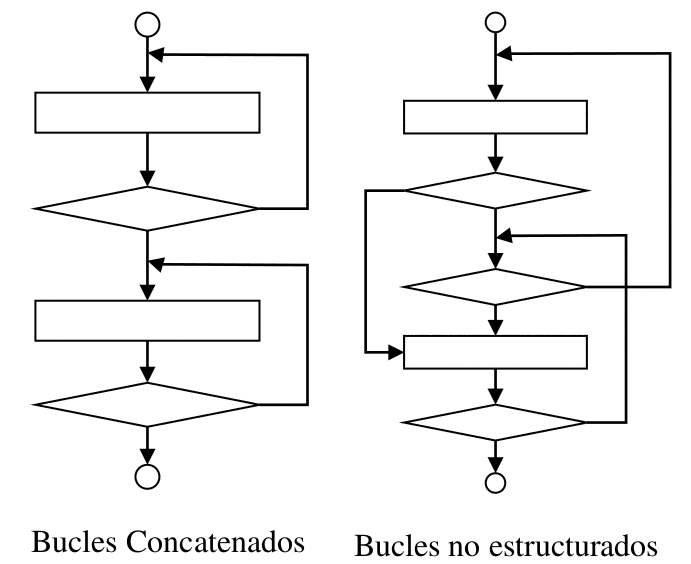
\includegraphics[width=0.5\linewidth]{Resources/Tema6/Ejemplo_BucleNoEstructurado.png}
    \caption{Ejemplificación de dos bucles. El izquierdo se ajusta a la programación estructurada, mientras que el derecho no lo hace.}
\end{figure}

\subsection{Utilización de la complejidad ciclomática de \textit{McCabe}}

La métrica de \textit{McCabe} es un \textbf{indicador del número de caminos independientes que existen en un grafo}; dicho de otro modo, trata de determinar, dado un grafo, cuántos caminos son precisos para probarlo. Se basa en la teoría de grafos. Por extensión, esta métrica también proporciona una medida cuantitativa de la complejidad lógica del módulo de software que se está probando.\\

El propio \textit{McCabe} definió como un buen criterio de prueba la consecución de la ejecución de un conjunto de caminos independientes igual al indicado por la métrica; es más, la métrica de \textit{McCabe} coincide con el número máximo de caminos independientes que puede haber un grafo. Cabe destacar que \textbf{un camino es independiente de otros si incorpora un arco que los demás no incluyen}.\\

Además, el conjunto de caminos que permite establecer asegura que todo el código se ejecuta, al menos, una vez, por lo que cubriría la cobertura de sentencias. Este criterio también se ha propuesto como equivalente a la cobertura de decisiones, pero han surgido contraejemplos que lo invalidan.\\

La complejidad de \textit{McCabe}, $V (G)$, puede ser calculada de tres maneras distintas a partir de un grafo de flujo $G$:
\begin{enumerate}
    \item $V (G) = a-n+2$, siendo $a$ el número de arcos, y $n$ el de nodos.
    \item $V (G) = r$, siendo $r$ el número de regiones cerradas del grafo.
    \item $V (G) = c+1$, siendo $c$ el número de nodos de condición. Una condición de $n$ arcos de salida se contabiliza cono $n-1$ (si $n>2$, equivale al número de bifurcaciones binarias necesarias para simular dicha bifurcación \textit{n-aria}).
\end{enumerate}

\begin{figure}[H]
    \centering
    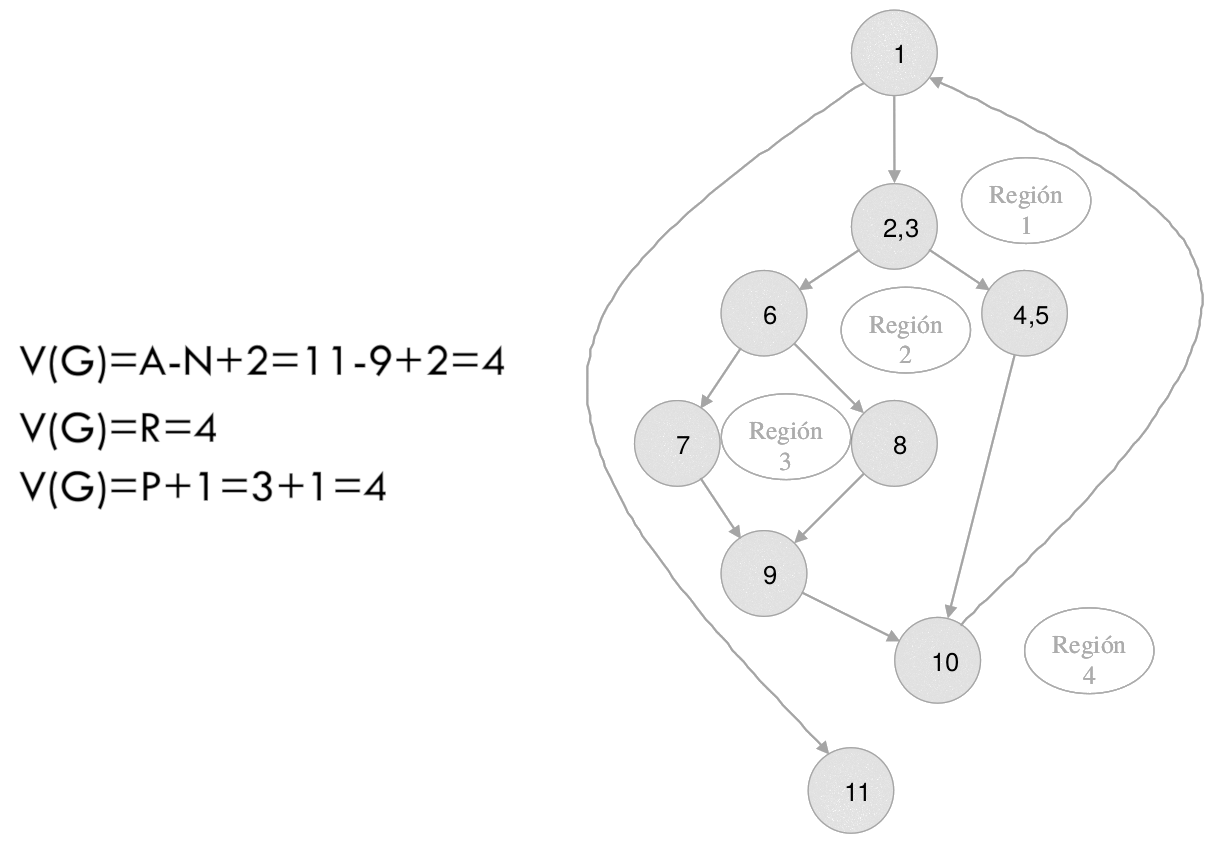
\includegraphics[width=0.9\linewidth]{Resources/Tema6/Ejemplo_McCabe.png}
    \caption{Primer ejemplo del cálculo de la complejidad ciclomática de \textit{McCabe}.}
\end{figure}

\begin{figure}[H]
    \centering
    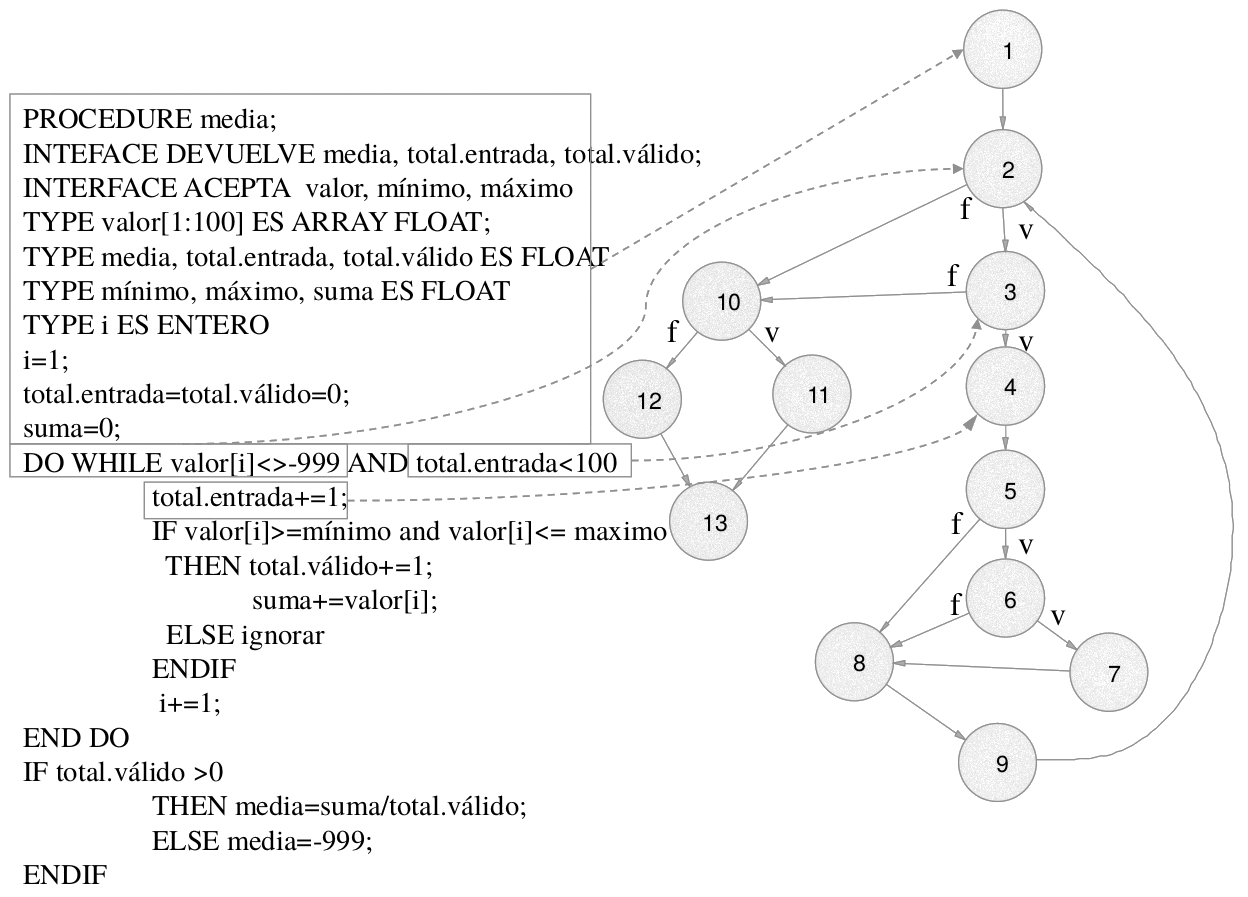
\includegraphics[width=0.9\linewidth]{Resources/Tema6/Ejemplo_CalculoComplejidadCiclomatica.png}
    \caption{Segundo ejemplo del cálculo de la complejidad ciclomática de \textit{McCabe}; los correspondientes resultados se encuentran inmediatamente debajo de esta descripción. Ahora, no solo se muestra un grafo de flujo, sino también el método a partir del cual se ha obtenido.}
\end{figure}

\paragraph{Complejidad de \textit{McCabe}}

\begin{enumerate}
    \item $V (G) = a-n+2 = 17-13+2 = 6$.
    \item $V (G) = r = 6$.
    \item $V (G) = c+1 = 5+1 = 1$.
\end{enumerate}

\textbf{Nota:} \textit{Hay que tener presente, para el número de regiones, que la fórmula solo es aplicable a grafos fuertemente conexos (siempre existe un camino para cualesquiera dos nodos que se escojan). Esto no se verifica en los programas con un nodo de inicio y otro de fin, por lo que, para calcular las regiones, o bien es necesario unir estos nodos, o bien debe contabilizarse la región externa.}\\

Una vez calculado del valor de $V (G)$, permitiendo afirmar por lo tanto el número máximo de caminos independientes del grafo $G$, para ayudar a la elección de los caminos de prueba, \textit{McCabe} propone el \textbf{método del camino básico} para la selección de los caminos independientes. Consiste en:

\begin{enumerate}
    \item Se escoge un camino de prueba típico (básico).
    \item Se crean variaciones sobre el camino, de forma que cada una de ellas se distinga en, al menos, una arista de las demás.
    \item Una vez seleccionados los caminos, se analiza el código para determinar las entradas que los fuerzan.
    \item Finalmente, se revisa la especificación para predecir las salidas correctas (en teoría) ante las entradas determinadas.
\end{enumerate}

Es conveniente tener presente que algunos caminos no se podrán ejecutar solos, sino que requerirán la ejecución de algún otro. Además es posible que, para un camino, no exista un conjunto de entradas que lo fuercen, por lo que deberá ser sustituido por otro para seguir satisfaciendo el criterio de \textit{McCabe}.\\

\textbf{Nota:} \textit{$V (G)$ marca un límite mínimo de número de casos de prueba para un programa. Si $V (G)$ es mayor que 10, la probabilidad de encontrar defectos en el módulo aumenta por presentar una elevada complejidad (salvo que sea debido a sentencias \textit{switch case} o similares); en estos casos, debería replantearse el diseño del módulo.}


\section{Pruebas funcionales (de caja negra)}

Estas pruebas se centran en el \textbf{estudio de la especificación del software}; es decir, conocidas las entradas, es posible determinar las salidas esperadas, y el flujo de datos interno no importa. Se tratará de encontrar errores en las siguientes categorías mediante las pruebas de caja negra:

\begin{itemize}
    \item Funciones incorrectas o ausentes.
    \item Errores de interfaz.
    \item Errores en estructuras de datos o accesos a bases de datos.
    \item Errores de rendimiento.
    \item Errores de inicialización y terminación.
\end{itemize}

De nuevo, la prueba exahustiva es generalmente impracticable, por lo que deben buscarse criterios que permitan elegir un subconjunto de casos cuya ejecución aporte una cierta confianza en detectar los posibles defectos del software.\\

Existen dos enfoques a la hora de seleccionar casos de prueba de caja negra.

\subsection{Enfoque sistemático}

El diseño de pruebas se apoyará en las siguientes dos definiciones de \textit{Myers} para buscar \uline{buenos casos de prueba} (presentan una alta probabilidad de detectar un nuevo error):

\begin{itemize}
    \item \textbf{El caso ejecuta el máximo número de posibilidades de entrada diferentes} para reducir así el total de casos adicionales necesarios.
    \item \textbf{Cada entrada cubre un conjunto extenso de otras}. Además de dar información sobre la ausencia o presencia de defectos con las entradas probadas, estos resultados pueden ser generalizados con cierta seguridad para otro conjunto de entradas similares que no hayan sido probadas.
\end{itemize}

\subsubsection{Partición o clases de equivalencia}

Esta técnica de diseño de casos se basa en \textbf{dividir el dominio de valores de entradas} en un número finito de clases, de modo que \textbf{la prueba de un valor representativo de una clase permite suponer}, razonablemente, que \textbf{el resultado obtenido será ``el mismo''} que el obtenido probando cualquier otro valor de la clase.\\

Para ello, hay que realizar las siguientes tareas:

\begin{enumerate}
    \item \textbf{Identificar las posibles clases de equivalencia a partir de la especificación del programa}. Consta de los siguientes pasos:
    
    \begin{enumerate}[a.]
        \item \textbf{Identificar las condiciones de las entradas del programa}; es decir, las restricciones de formato y posibles valores de las entradas.
        
        \item \textbf{Identificar, a partir de ellas, las clases de equivalencia}, que pueden ser (1) de datos válidos, o (2) de datos no válidos o erróneos. Esta identificación debe realizarse, como ya se comentó, basándose en el principio de igualdad de tratamiento de los valores de cada clase.\\
        
        Existen algunas \uline{reglas} que ayudan a identificar clases:

        \begin{enumerate}[R1.]
            \item Si se especifica un rango de valores, se creará una clase válida y dos clases no válidas. \textit{Por ejemplo: $5<n<7$.}
            \item Si se especifica una lista de valores de tamaño variable, se creará una clase válida y dos no válidas. \textit{Por ejemplo: puede haber de 1 a 4 titulares para una cuenta bancaria.}
            \item Si se especifica una situación del tipo \textit{debe ser} o booleana, se creará una clase válida y una no válida. \textit{Dos ejemplos serían: (1) que el primer carácter debe ser una letra, (2) o que la edad debe introducirse en formato numérico.}
            \item Si se especifica un conjunto de valores admitidos, que son tratados de forma distinta, se creará una clase válida por cada valor, y una clase no válida. \textit{Por ejemplo: pueden registrarse tres tipos de inmuebles, siendo chalets, pisos, o locales comerciales.}
            \item En cualquier caso, si se sospecha que ciertos elementos de una clase no se tratan igual que el resto de la misma, deben dividirse en clases menores.
        \end{enumerate}
    \end{enumerate}

    \item \textbf{Crear los casos de prueba correspondientes}. Consta de las siguientes fases:
    
    \begin{enumerate}[a.]
        \item Asignar un número único a cada clase de equivalencia.
        \item Hasta que todas las clases de equivalencia hayan sido cubiertas por casos de prueba, se tratará de escribir un caso que cubra tantas clases válidas no incorporadas como sea posible.
        \item Hasta que todas las clases de equivalencia no válidas hayan sido cubiertas, se escribe un caso para cada una de las clases no válidas sin cubrir.\\
        
        El motivo de cubrir, con casos individuales, las clases no válidas, es que \uline{ciertos controles de entrada pueden enmascarar o invalidar otros controles similares}. Por ejemplo, en un programa donde hay que \textit{introducir cantidad (1--99) y letra inicial (A--Z)}, ante el caso \textit{105} \texttt{\&} (dos errores), se puede indicar solo el mensaje \textit{105 fuera de rango}, y dejar sin examinar el resto de la entrada a pesar de ser también inválida. Esto sería incluso más peligroso si el programa respondiese con un mensaje ambiguo, como \textit{dato incorrecto, introduzca valor}, dado que podría llevar a pensar al equipo de pruebas a que ambos errores fueron correctamente identificados.
    \end{enumerate}
\end{enumerate}

\subsubsection{Análisis de valores límite (ALV)}

Mediante la experiencia, se ha podido constatar que los \textbf{los casos de prueba que exploran las condiciones límite de un programa producen un mejor resultado para la detección de defectos}. Las condiciones límite se pueden definir como \uline{las situaciones que se hayan directamente arriba, abajo, y en los márgenes de las clases de equivalencia}.\\

Realmente, esta técnica de diseño de casos complementa a la de particiones. Las diferencias entre ellas son:

\begin{itemize}
    \item En lugar de elegir ``cualquier'' elemento como representativo de una clase de equivalencia, se requiere que se escojan uno o más elementos tal que los márgenes se somentan a prueba.
    \item En lugar de concentrarse únicamente en el dominio de entradas, los casos de prueba se generan considerando también el espacio de salida.
\end{itemize}

De nuevo, el proceso de selección es heurístico, como en la técnica de particiones, pero existen ciertas reglas orientativas:

\begin{enumerate}[R1.]
    \item Si una condición de entrada especifica un intervalo cerrado de valores (\textit{por ejemplo: $[-1.0, 1.0]$}), se deben generar casos para los extremos del rango (\textit{$-1.0$ y $1.0$}), y casos no válidos para situaciones justo más allá de los extremos (\textit{$-1.001$ y $1.001$, en el caso de que se admitan tres decimales}).
    \item Si la condición de entrada especifica un número de valores (por ejemplo: \textit{el fichero de entrada tendrá de 1 a 255 registros}), se diseñarán casos para (1) el valor máximo, (2) el valor mínimo, (3) uno más que el máximo, y (4) uno menos que el mínimo (\textit{en este caso, $0, 1, 255, 256$}).
    \item Usar la regla R1 para la condición de salida. \textit{Por ejemplo: si el descuento máximo aplicable en una compra será el 50\%, y el mínimo será el 6\%, se escribirán casos para intentar obtener descuentos de 5.99\%, 6\%, 50\%, y 50.01\%}.
    \item Usar la regla R2 para cada condición de salida. \textit{Por ejemplo: si el programa puede mostrar de 1 a 4 listados, se escribirán casos para intentar generar 0, 1, 4, y 5 listados.}\\
    En esta regla, como en la R3, debe recordarse que:
    \begin{itemize}
        \item Los valores límite de entrada no generan necesariamente los valores límite de salida.
        \item No siempre se pueden generar resultados fuera del rango de salida, pero la posibilidad debe ser considerada igualmente.
    \end{itemize}
\end{enumerate}

Además, como norma general, si la entrada o salida de un programa es un conjunto ordenado, los casos deben concentrarse en el primer y último elemento. \textit{Por ejemplo: una tabla, o un archivo secuencial.}

\subsubsection{Conjetura de errores}

La idea básica de esta técnica consiste en \textbf{enumerar una lista de equivocaciones que pueden cometer los desarrolladores}, para después generar casos de prueba por cada uno de los elementos en ella. No existen directivas eficaces, ya que la lista será creada en base a la intuición y la experiencia; sin embargo, algunos valores a tener en cuenta son:

\begin{itemize}
    \item El valor cero, tanto en la entrada como en la salida.
    \item En situaciones en las que se introduce un número variable de valores, conviene centrarse en los casos de (1) que no haya ningún valor, (2) que solo haya uno, y (3) que todos los valores sean iguales.
    \item Es recomendable imaginar que el desarrollador pudiera haber interpretado algo mal en la especificación.
    \item También interesa imaginar lo que el usuario pueda introducir como entrada a un programa, previniendo toda clase de acciones, incluso como si el usuario fuese poco hábil, o que pudiese presentar malas intenciones.
\end{itemize}

\subsection{Enfoque aleatorio}

Se basa en la generación de pruebas aleatorias, en las cuales \textbf{se simula la entrada habitual del programa creando los datos de entrada en la secuencia y frecuencia con las que podrían aparecer en la práctica}. Generalmente, el objetivo de estos llamados \uline{tests de esfuerzo} es el \textbf{evaluar el rendimiento del sistema}, puesto que, como las entradas son generadas aleatoriamente, no se pueden precedir las salidas. Esto es debido a que, si por el contrario contásemos con un software que predijese las salidas con total fiabilidad, este podría reemplazar directamente al software que está siendo probado.\\

Para crear estos tests, es necesario contar con una herramienta generadora de pruebas, a la que se especifica la descripción de las entradas, las secuencias de entrada posibles, y las probabilidades de ocurrir en la práctica (\textit{por ejemplo: indicando una distribución estadística si la siguen}). Si el proceso de generación se ha realizado correctamente, eventualmente se crearán todas las posibles entradas del programa, en todas las posibles combinaciones y permutaciones. 

\subsection{Métodos de prueba basados en grafos}

El primer paso en la prueba de caja negra es \textbf{entender los objetos que se modelan en el software y las relaciones entre ellos}. Una vez realizado todo esto, se continúa definiendo una serie de pruebas que verifiquen que \uline{todos los objetos tienen, entre ellos, las relaciones esperadas}. Dicho de otra manera, la prueba del software empieza creando un grafo de objetos importantes y sus relaciones, y después \textbf{diseñando una serie de pruebas que cubran el grafo de manera que se ejerciten todos los objetos y sus relaciones} para descubrir los errores.\\

Para llevar a cabo estos pasos, debe comenzarse creando el grafo, que representará:

\begin{itemize}
    \item Objetos mediante sus nodos.
    \item Relaciones entre los objetos mediante los arcos.
    \item Propiedades de un objeto mediante el peso de su correspondiente nodo.
    \item Características de las relaciones mediante el peso de su correspondiente arco.
\end{itemize}

\begin{figure}[H]
    \centering
    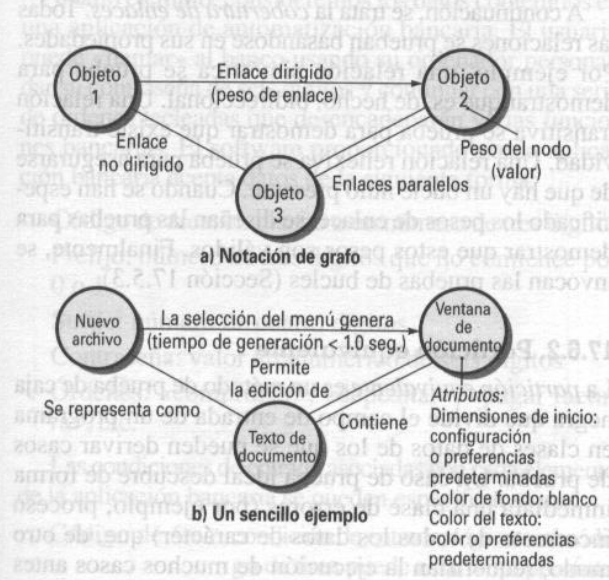
\includegraphics[width=0.5\linewidth]{Resources/Tema6/Ejemplo_Grafo.png}
    \caption{Representación simbólica de un grafo para pruebas de caja negra.}
    \label{fig:estrategiasPruebas}
\end{figure}

Una vez creado el grafo, se puede proceder a la creación de los casos de prueba. Entre los beneficios que este tipo de grafos aporta a este procedimiento, se encuentra el facilitar:

\begin{itemize}
    \item La identificación de los bucles a probar.
    \item El cumplimiento de la cobertura de nodos, de modo que ninguno haya sido omitido.
    \item El cumplimiento de la cobertura de enlace, probándose todas y cada una de las relaciones. Cada relación debe ser probada basándose en sus propiedades:
    \begin{itemize}
        \item Se estudia la transitividad de las relaciones secuenciales para determinar cómo se propaga el impacto de las relaciones a través de los objetos definidos en el grafo.
        \item La simetría de una relación también es importante para el diseño de casos de prueba; si un enlace es bidireccional, debería probarse esta característica.
        \item Todos los nodos del grafo deberían ser reflexivos; es decir, tener una relación que los devuelva a ellos mismos. % No estoy seguro, ya estaba escrito por el autor original, y los apuntes no profundizan en ello.
    \end{itemize}
\end{itemize}

A continuación, se describe un número de métodos de prueba de comportamiento que pueden hacer uso de los grafos:

\begin{itemize}
    \item \textbf{Modelado del flujo de transacción:} Los nodos representan los pasos de alguna transacción, y los enlaces son las conexiones lógicas entre ellos; sería posible partir de un DFD. \textit{Por ejemplo: los pasos requeridos para hacer una reserva en un hotel; son pasos del proceso, se use software o no.}
    \item \textbf{Modelado de estados finitos:} Los nodos son estados del software observables por el usuario, y los enlaces representan las transiciones que ocurren para moverse de un estado a otro. \textit{Por ejemplo: el usuario puede interactuar con pantallas, sobre las cuales realizar acciones que lleven a otras pantallas.}
    \item \textbf{Modelado del flujo de datos:} Los nodos son objetos de datos, y los enlaces son las transformaciones que sufren para pasar de ser un objeto a otro.
\end{itemize}

Es importante tener presente que \textbf{todos son modelos de caja negra}, por lo que no modelan cómo está programado el software; es decir, no modelan ni los estados del software, ni sus transacciones programadas, ni sus flujos de datos. En realidad, \textbf{modelan su comportamiento visible}.


\section{Enfoque práctico recomendado para el diseño de casos}

El enfoque recomendado para el uso de las técnicas de diseño de casos pretende mostrar el uso más apropiado de cada técnica para la obtención de un conjunto de casos útiles sin perjuicio de las estrategias de niveles de prueba.

\begin{enumerate}
    \item \textbf{Si la especificación contiene combinaciones de condiciones de entrada, se comienza formando sus grafos causa--efecto} para comprenderlas con más facilidad.
    \item \textbf{Se identifican las clases válidas y no válidas de equivalencia para la entrada y la salida}.
    \item En todos los casos, \textbf{se usa el análisis de valores límite (AVL) para añadir casos de prueba}.
    \item \textbf{Se utiliza la conjetura de errores para añadir nuevos casos}, principalmente referidos a valores especiales.
    \item \textbf{Se ejecutan los casos generados hasta el momento (de caja negra), y se analiza la cobertura obtenida}.
    \item \textbf{Se examina la lógica del programa para añadir los casos precisos (de caja blanca) para cubrir el criterio de cobertura elegido}, siempre y cuando no haya sido satisfecho en el anterior punto.
\end{enumerate}


\section{Documentación del diseño de las pruebas (IEEE 829)}

Conviene tener siempre presente que \textbf{la documentación de las pruebas es necesaria para una buena organización de las mismas, así como para asegurar su reutilización}.\\

Según el estándar \textbf{estándar IEEE 829}, se generará la siguiente documentación:

\begin{figure}[H]
    \centering
    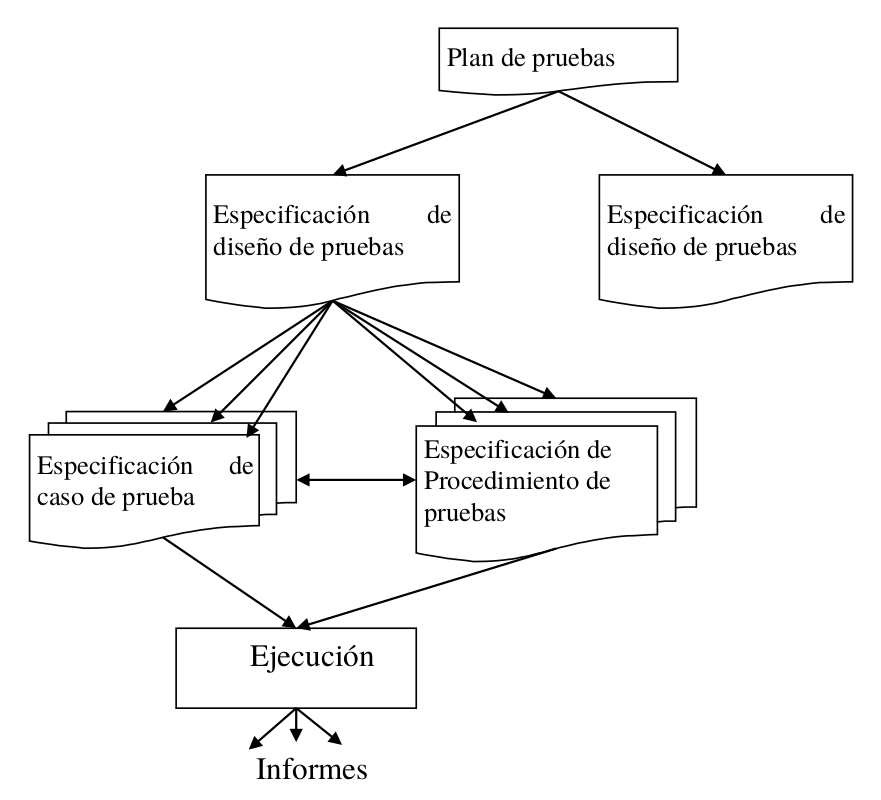
\includegraphics[width=0.6\linewidth]{Resources/Tema6/IEEE_829.png}
    \caption{Representación de los documentos del estándar IEEE 829 para la documentación del diseño de pruebas.}
    \label{fig:IEEE829}
\end{figure}

\begin{enumerate}
    \item \textbf{Plan de pruebas}: El documento tiene el objetivo de mostrar la planificación general del esfuerzo para cada fase de la estrategia de prueba del producto. Parte de los elementos fijados en el estándar son:
    \begin{enumerate}
        \item Una introducción y resumen de los elementos y características a probar.
        \item Los elementos de software a probar (programas o módulos).
        \item Qué características se van a probar y cuáles no.
        \item Actividades, técnicas, herramientas\ldots
        \item Criterios de paso/fallo para cada elemento.
        \item Documentos a entregar.
        \item Actividades de preparación y ejecución de las pruebas.
        \item Necesidades del entorno.
        \item Responsables de la realización de las pruebas, y sus necesidades.
        \item Esquema de tiempos y riesgos asumidos.
    \end{enumerate}

    \item \textbf{Especificación del diseño de pruebas}: Partiendo del plan de pruebas, se realizan ampliaciones de los detalles mostrados, especificando un diseño de prueba por cada módulo del programa. En el estándar se fija la siguiente estructura:
    \begin{enumerate}
        \item Las características a probar de los elementos sofware.
        \item Detalles sobre el plan de pruebas creado, incluyendo las técnicas de prueba específicas y los métodos de análisis de resultados.
        \item Se identifica cada prueba: Identificador, casos que se van a utilizar, y procedimientos que se van a seguir.
        \item Criterios de paso y fallo de la prueba.
    \end{enumerate}

    \item \textbf{Especificación del caso de prueba}: A partir del anterior diseño, se definen con detalle cada uno de los casos de prueba mencionados, especificando datos de pruebas exactos, resultados esperados, y demás detalles, para obtener un conjunto de pruebas de validación y de verificación. En el estándar se fija la siguiente estructura:
    \begin{enumerate}
        \item Elementos software a probar, y cuáles de sus características serán ejercitadas por el caso.
        \item Especificaciones de cada entrada requerida para ejecutar el caso. Deben detallarse además las relaciones entre estas; \textit{por ejemplo: la sincronización de las mismas.}
        \item Especificaciones de todas las salidas y las características requeridas (\textit{por ejemplo: el tiempo de respuesta}).
        \item Necesidades del entorno. \textit{Por ejemplo: en cuanto a hardware, software, o personal}.
        \item Requisitos o restricciones especiales de procedimiento.
        \item Dependencias entre casos.
    \end{enumerate}

    \item \textbf{Especificación del procedimiento de prueba}: Tras generar los casos de prueba detallados, se especifica cómo proceder en detalle a su ejecución. En el estándar se fija la siguiente estructura:
    \begin{enumerate}
        \item Objetivo del procedimiento y lista de casos que se ejecutan con él.
        \item Requisitos especiales para la ejecución.
        \item Pasos en el procedimiento. Además de la manera de registrar los resultados y los incidentes de la ejecución, se debe especificar:
        \begin{itemize}
            \item La secuencia necesaria de acciones para preparar la ejecución.
            \item Acciones necesarias para empezar la ejecución.
            \item Acciones necesarias durante la ejecución.
            \item Cómo se realizarán las medidas. \textit{Por ejemplo: del tiempo de respuesta.}
            \item Cómo tratar incidencias y restaurar el entorno de ejecución.
        \end{itemize}
    \end{enumerate}
\end{enumerate}


\section{Ejecución de las pruebas}

\subsection{El proceso de ejecución (IEEE 1008)}

El proceso abarca las siguientes fases:

\begin{figure}[H]
    \centering
    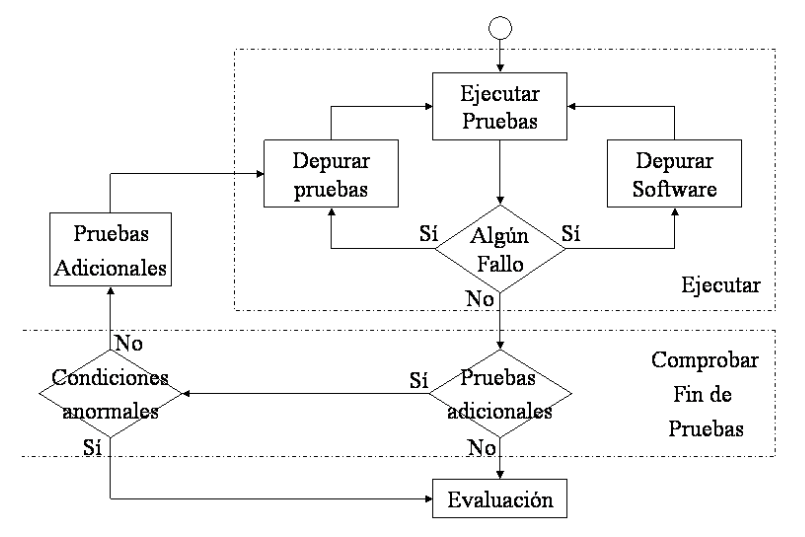
\includegraphics[width=0.75\linewidth]{Resources/Tema6/IEEE_1008.png}
    \caption{Representación de proceso de pruebas según el estándar IEEE 1008.}
\end{figure}

\begin{enumerate}
    \item \textbf{Proceso de ejecución}: Se ejecutan las pruebas, cuyos casos y procedimientos han sido ya diseñados previamente. Consta de las siguientes fases:
    \begin{enumerate}
        \item Se ejecutan las pruebas.
        \item Se comprueba si ha habido algún fallo al ejecutar que impida terminar la ejecución de algún caso; dicho de otro modo, se comprueba si las pruebas no han podido terminar. \textit{Por ejemplo: se cae el sistema, se bloquea el teclado\ldots}
        \item Si lo ha habido, se puede deber a un defecto software, que llevará a la depuración o corrección del código, o a un defecto en el propio diseño de las pruebas. En ambos casos, \uline{las nuevas pruebas} (quizá cambien al corregir el software) o \uline{las corregidas deberán ejecutarse}.
        \item De no existir fallo, se pasará a la comprobación de la terminación de las pruebas.
    \end{enumerate}

    \item \textbf{Comprobación de la conclusión del proceso de prueba}: Se lleva a cabo según criterios de compleción de prueba que suelen ser especificados en el plan de pruebas. Consta de las siguientes fases:
    \begin{enumerate}
        \item Tras la ejecución, se comprobará si se cumplen los criterios de compleción descritos en el correspondiente plan de pruebas. \textit{Por ejemplo: se terminan las pruebas cuando se han probado todos los procedimientos de operación, o se ha cumplido la cobertura lógica marcada.}
        \item En caso de terminar las pruebas, se pasa a la \uline{evaluación de los resultados obtenidos}. \textit{Se alcanza una terminación normal.}
        \item En caso de no terminar las pruebas, se debe comprobar la presencia de condiciones anormales en la prueba.
        \begin{itemize}
            \item Si se hubiesen dado condiciones anormales (\textit{por ejemplo: no se han podido ejecutar todos los casos porque el sistema se cae regularmente}), se pasa de nuevo a la \uline{evaluación}; dicho de otro modo, las pruebas no se han pasado, pero no ha sido culpa del software. \textit{Se alcanza una terminación anormal}.
            \item En caso contrario, se pasa a \uline{generar y ejecutar pruebas adicionales para satisfacer cualquiera de las dos posibles terminaciones} de las pruebas.
        \end{itemize}
    \end{enumerate}
\end{enumerate}

\subsection{Documentación de la ejecución de las pruebas}

La documentación de la ejecución de las pruebas también es fundamental para dejar constancia de los resultados de las pruebas. \uline{Parte de los documentos generados se relacionan directamente con el estándar IEEE 829}, pudiéndose distinguir dos grupos principales:

\begin{itemize}
    \item \textbf{Documentación de entrada}: Constituida principalmente por las especificaciones de los casos de prueba que se van a usar, y las especificaciones de los procedimientos de pruebas.
    
    \item \textbf{Documentación de salida o informes sobre la ejecución}: Cada ejecución generará dos tipos de documentos.
    \begin{itemize}
        \item \textbf{Histórico de pruebas} (\textit{test log}): Documenta todos los hechos relevantes ocurridos durante la ejecución de las pruebas. La estructura fijada en el estándar es:
        \begin{itemize}
            \item Descripción de la prueba, detallando los elementos probados y el entorno de prueba.
            \item Anotaciones de datos sobre cada hecho ocurrido, incluidos el inicio y fin de la prueba: Fecha, hora, e identificador del informe de incidente asociado, en caso de haberlo.
            \item Otras informaciones.
        \end{itemize}
        \item \textbf{Informes de los incidentes ocurridos} (\textit{test incident report}), siempre en caso de que sucedan durante la ejecución: Cada uno documenta un incidente que requirá una posterior investigación. La estructura fijada en el estándar es:
        \begin{itemize}
            \item Resumen del incidente.
            \item Descripción de datos objetivos: Fecha, hora, entradas, resultados esperados, etc.
            \item Impacto que tendrá sobre las pruebas.
        \end{itemize}
    \end{itemize}
    Además, \textbf{toda la documentación de salida correspondiente a un mismo diseño de prueba se recoge en un informe resumen de pruebas} (\textit{test summary report}), resumiéndose así los resultados de las actividades de prueba, y \uline{aportándose una evaluación del software} basada en ellos. Entre otros elementos a incluir en el informe, destacan:
    \begin{itemize}
        \item Resumen de la evaluación de los elementos probados.
        \item Variaciones del software respecto a su especificación de diseño, así como las variaciones en las pruebas.
        \item Valoración de la extensión de la prueba. \textit{Cobertura lógica, funcional, de requisitos, etc.}
        \item Resumen de cada una de las actividades de prueba, incluyendo detalles sobre los recursos empleados.
    \end{itemize} 
\end{itemize}

\textbf{Nota:} \textit{Cada uno de los documentos detallados anteriormente, tanto para la documentación del diseño de las pruebas, como para la ejecución de estas, debe contar con un identificador.}

\subsection{Depuración}
La depuración es el \textbf{proceso de localizar, analizar y corregir los defectos que se sospecha que contiene el software}. Suele ser la consecuencia de una prueba con éxito, que conlleva mandar un módulo a depuración. De este modo, el proceso de depuración puede \uline{dar lugar a dos situaciones}:

\begin{itemize}
    \item \textbf{Encontrar la causa del error, analizarla y corregirla}.
    \item \textbf{No encontrar la causa} y, por lo tanto, tener que \textbf{generar nuevos casos de prueba que puedan proporcionar información adicional} para su localización.
\end{itemize}

Por lo tanto, se puede distinguir las \uline{dos fases} siguientes:

\begin{itemize}
    \item \textbf{Localización del defecto}: Suele conllevar la mayor parte del esfuerzo.
    \item \textbf{Corrección del defecto}.
\end{itemize}

Además, tras corregir el efecto, \uline{deberán efectuarse nuevas pruebas que comprueben si este ha sido efectivamente eliminado}.

\begin{figure}[H]
    \centering
    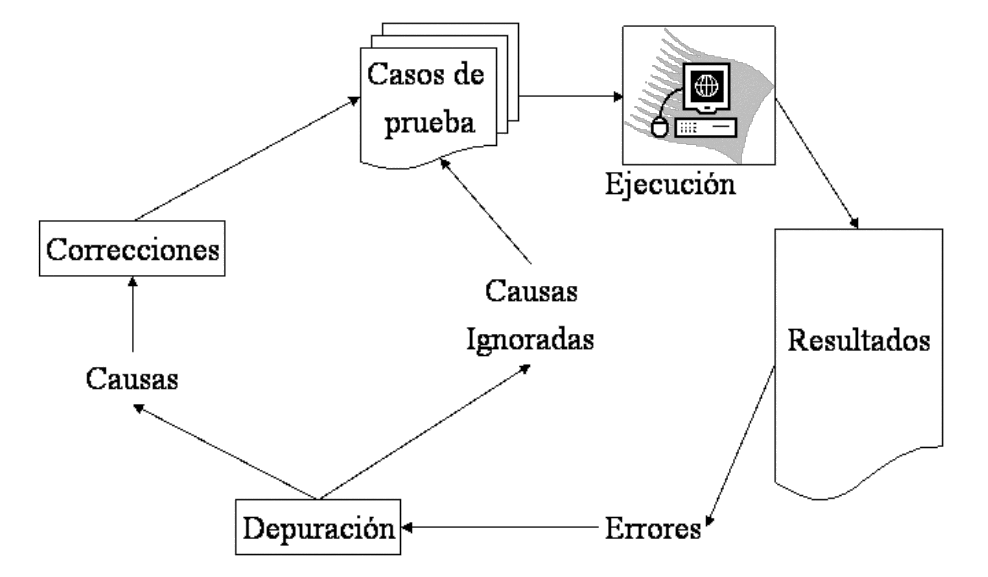
\includegraphics[width=0.7\linewidth]{Resources/Tema6/ProcesoDepuracion.png}
    \caption{Representación de proceso de depuración.}
\end{figure}

\subsubsection{Consejos para la depuración}

\begin{itemize}
    \item \textbf{Para la localización del error:}
    \begin{itemize}
        \item Es el proceso mental de solución de un problema. Por ello, debería analizarse la información disponible, en lugar de explorar aleatoriamente o experimentar cambiando el programa.
        \item Las herramientas de depuración deberían emplearse como recurso secundario.
        \item Al llegar a un punto muerto, puede merecer la pena pasar a otra cosa para refrescar la mente, e incluso puede ayudar el describir el problema a otra persona.
        \item Se deben atacar los errores individualmente, o solo se dificultará la depuración.
        \item Se debe fijar la atención también en los datos manejados, y no solo en la lógica del proceso.
    \end{itemize}

    \item \textbf{Para la corrección del error:}
    \begin{itemize}
        \item Donde hay un defecto, suele haber más (\textit{ejemplo del Principio de Pareto}).
        \item Debe corregirse el defecto, en lugar de intentar enmascarar sus síntomas.
        \item La probabilidad de corregir un defecto perfectamente no es el 100\%, por lo que las correciones deben ser revisadas antes de implantarlas.
        \item Debe tenerse cuidado para no crear nuevos defectos como consecuencia de realizar correcciones sin cautela.
        \item La corrección debe situarnos temporalmente en la fase de diseño, para alterar el diseño correspondiente al código defectuoso.
    \end{itemize}
\end{itemize}

\subsection{Análisis de errores a análisis causal}

El objetivo del análisis causal es \textbf{proporcionar información sobre la naturaleza de los defectos, para que así el personal pueda prevenirlos en el futuro}, al conocer los errores que comete; esta información no debe ser empleada nunca para evaluar al personal.\\

Se recoge la siguiente información:
\begin{itemize}
    \item Cuándo se cometió.
    \item Quién lo cometió.
    \item Qué se hizo mal.
    \item Cómo se podría haber prevenido.
    \item Por qué no se detectó antes.
    \item Cómo se podría haber detectado antes.
    \item Cómo se encontró el error.
\end{itemize}


\section{Estrategia de aplicación de las pruebas}

Una vez conocidas las técnicas de diseño y de ejecución, se debe analizar \uline{cómo se plantea la utilización de las pruebas en el ciclo de vida}. La estrategia de aplicación y la planificación de las pruebas \textbf{pretenden integrar el diseño de los casos de prueba y permiten la coordinación del personal y del cliente}, gracias a la definición de los papeles que debe desempeñar cada uno de ellos, así como de la forma de llevarlos a cabo.\\

Las etapas de las que constaría la estragia serían:

\begin{figure}[H]
    \centering
    \includegraphics[width=0.7\linewidth]{Resources/enfoquePruebas}
    \caption{Las diferentes estrategias de prueba y su relación con las otras fases de la construcción del software}
    \label{fig:estrategiasPruebas}
\end{figure}

\begin{enumerate}
    \item \textbf{Se comienza en la prueba de cada módulo}, realizada normalmente por el propio personal de desarrollo.
    \item Con el esquema del diseño del software, \textbf{los módulos probados se integran para comprobar sus interfaces}.
    \item \textbf{El software totalmente ensamblado se prueba como un conjunto} para comprobar si cumple o no tanto los requisitos funcionales como los requisitos de rendimientos, seguridad, etc. Este nivel \uline{coincide con la prueba del sistema cuando este solo se trata de software}.
    \item El caso de que el sistema final conste de más que software, \textbf{el software ya validado se integra con el resto del sistema} (\textit{por ejemplo: elementos mecánicos}), \textbf{para probar su funcionamiento conjunto}. \textit{Por extensión, todavía es posible simular el hardware implicado en la anterior etapa. El resultado de esta fase es la certeza de haber hecho lo deseado, además de haberlo hecho bien.}
    \item Finalmente, \textbf{el producto final se pasa a la prueba de aceptación para que el usuario compruebe, en su propio entorno de explotación, si lo acepta o no}. \textit{El resultado de esta fase es que el usuario tenga la certeza de recibir lo que él quería}.
\end{enumerate}

Como se puede ver, \uline{cada nivel de prueba se centra en probar el software en referencia al trabajo realizado en una diferente etapa de desarrollo}.\\

\textbf{Nota:} \textit{Las pruebas de aceptación, de sistema, y de integración están relacionadas directamente con las pruebas de validación. Por otra parte, las pruebas de integración (se encuentra en ambos bandos) y de unidad se encuentran directamente relacionadas con las pruebas de verificación. De todos modos, una prueba de módulo puede centrarse también en la especificación de las funciones que este debe realizar (de caja negra).}\\

\textbf{Nota:} \textit{A pesar de que un ciclo en cascada tenga una fase de pruebas, estas suelen distribuirse a lo largo de todo el ciclo de vida.}\\


\section{Pruebas en desarrollos orientados a objetos (\textit{OO})}

Las técnicas y estrategias presentadas hasta el momento están inspiradas en la aplicación a desarrollos estructurados. Por lo tanto, al trabajar con tecnología \textit{OO}, algunas de ellas pierden su interés o deben adaptarse.\\

\subsection{Punto de vista del diseño de casos de pruebas}

\begin{itemize}
    \item \textbf{Técnicas de caja negra}: Siguen siendo completamente válidas. \textit{Por ejemplo: el AVL, el tratamiento de combinaciones de entrada, la conjetura de errores\ldots} Los casos de prueba deberían ser diseñados basándose en:
          \begin{itemize}
              \item Los datos y eventos incluidos en los escenarios de los casos de uso.
              \item Los caminos que se pueden trazar en los diagramas de actividad, o en los de estados, que describan el caso de uso, sin olvidar todos los flujos alternativos, ni los tratamientos de errores y excepciones.
          \end{itemize}
    \item \textbf{Técnicas de caja blanca}: Disminuyen sus posibilidades de aplicación, quedando confinadas a las instrucciones de cada método de cada clase. También cabría la posibilidad de aplicar la cobertura de caminos (incluido el criterio de \textit{McCabe}) no solo al código de los métodos, sino también a los diagramas de comportamiento con estructura de red; \textit{por ejemplo: diagramas de estados, de actividad, etc.}
\end{itemize}

En el caso del diseño de pruebas, cabe señalar además la posibilidad de \uline{distinguir criterios según el nivel de pruebas en el que se sitúe el diseño}. Así, para las pruebas de unidad (es decir, pruebas de clases), la prueba de clases de equivalencia y de AVL  son apropiadas aplicándolas a las entradas y salidas representadas como parámetros de métodos fundamentalmente. Sin embargo, \textbf{los cambios más radicales aparecen en las pruebas de integración}, dado que el enfoque de integración basado en la existencia de una estructura jerárquica no tiene sentido frente a las estructuras de colaboración en red definidas para el software \textit{OO}.\\

Por una parte, existen propuestas que permiten \uline{encontrar aquellas clases que dependen en su funcionamiento de sí mismas o solo de unas pocas clases, para tomarlas como destino de la primera oleada de pruebas de integración}, de modo que más adelante se irán sometiendo a prueba las clases que dependen solo de las ya probadas, y así consecutivamente hasta integrar toda la aplicación. Sin embargo, el enfoque más habitual consiste en \uline{ir probando hilos de clases que colaboran para una función o servicio del sistema}, seguramente definidos en diagramas de colaboración; los diagramas de estado pueden aportar una mayor información para el rigor de la prueba.

\subsection{Cuestiones a tener en cuenta}

Finalmente, se señalarán cuestiones que tienen una gran influencia en las pruebas de software \textit{OO}:

\begin{itemize}
    \item \textbf{Herencia}: Probar un método de la clase padre no garantiza su funcionamiento en clases hijas.
    \item \textbf{Polimorfismo}: Un único método puede tener implementaciones diferentes en función de la clase en la que se use, empeorando la preocupación del anterior punto.
    \item También es conveniente recordar que la propia programación o diseño \textit{OO} hace menos probables ciertos tipos de error y más probables otros, además de provocar la aparición de nuevos tipos de defectos, todo ello frente a los desarrollos estructurados.
\end{itemize}

\newpage

\part{Preguntas de examen}

\section{Resolución de preguntas cortas}
Las preguntas cortas consistirán en refutar sentencias falsas en base a vuestros conocimientos de la asignatura. En ningún caso se tratará de contar todo lo que sabéis sobre el punto en cuestión de que trate la frase sino sólo de rebatir la falacia con argumentos objetivos y precisos. Las respuestas de más de 10 líneas no serán evaluadas, ya que entiendo que siempre debería poder responderse como máximo en 5 o 6.

\subsubsection*{1. Las normas de procesos para la construcción del software sólo describen procesos que tienen por objetivo el desarrollo de código ejecutable.}
\textit{Todas las normas vistas describen procesos incluidos en todo el ciclo de vida del software. Las normas ISO 12207 e ISO/IEC 15504 incluyen entre sus procesos principales los de adquisición y suministro (gestionan la compra-venta); también incluyen los procesos de soporte (describen tareas de apoyo, no de construcción) y los de la organización, que ni siquiera tienen que ver con el desarrollo de un proyecto software concreto. De hecho la codificación se tratar sólo como una actividad del proceso de desarrollo en estas normas.
    \\
    También se puede hacer el mismo razonamiento con la norma IEEE 1074 que nos proporciona 4 secciones lógicas de las que sólo una tiene que ver con el desarrollo. Las otras tres tienen que ver con la selección del ciclo de vida, la gestión del proyecto y los procesos integrales, vinculados a asegurar la terminación y calidad de los procesos.}

\subsubsection*{2. Sólo el SEI americano ha mostrado interés en la generación de normas para la Ingeniería del Software debido a su carácter académico.}
\textit{Como se ha discutido indirectamente en la pregunta anterior, las normas del IEEE y la ISO/IEC acreditan la preocupación de otras instituciones, independientes del SEI, por la formalización de estas normas. Además estos estándares, como se demuestra en la explicación del CMMI, están orientados a su aplicación en las empresas a las que deben proporcionar un marco válido que evite el desarrollo ad hoc de aplicaciones.}

\subsubsection*{3. Pasar del modelo en cascada al modelo incremental no solucionó ningún problema de ingeniería pero permitió ganar más dinero a los programadores.}
\textit{El salto al modelo incremental evita la concepción monolítica del software que da el modelo en cascada. Propone un modelo iterativo que permite la evolución en sus requisitos, la mejora de la comunicación con el cliente y posibilita reducir el coste de los errores.}

\subsubsection*{4. Ante un problema ya resuelto el planteamiento siempre debe ser reprogramar otra solución pues seguro que será más eficiente.}
\textit{Si el problema está resuelto implica que el software ya existe. La conclusión de los análisis de coste realizados en prácticas y la discusión sobre el reuso hecha en clase, es que será más barato (y por tanto eficiente) comprarlo que reconstruirlo. Sólo debemos plantearnos construir cuando la funcionalidad que necesitamos no está recogida por el software disponible o se precisa una modificación significativa para adaptarlo. Evidentemente no se considera que la funcionalidad esté en la aplicación si ésta no la realiza con la calidad esperada.}

\subsubsection*{5. Los únicos riesgos posibles de un proyecto son económicos y técnicos}
\textit{Si bien estos riesgos importantes, existen otro tipo de riesgos que pueden resultar cruciales a la hora de desarrollar un proyecto. Es el caso de los riesgos geopolíticos, desastres naturales, realizar un mal análisis de requisitos, realizar una mala planificación, o el espionaje industrial.}

\subsubsection*{6. La única cualidad importante del analista es ser persuasivo para convencer al cliente de que el software que le desarrollamos era el que necesitaba.}
\textit{En tanto que la persuasión es cualidad importante y forma parte de una de las muchas dotes comunicativas que debe tener un analista, no es suficiente.
    \\
    Un analista debe ser capaz de comunicar y de extraer información de los clientes.\\
    Además, valiéndose de sus conocimientos técnicos y experiencia en el campo de la ingeniería del software, ser capaz de traducir ideas vagas de necesidades de software en un conjunto concreto de funciones y restricciones.
}

\subsubsection*{7. La especificación es un documento escrito en lenguaje natural que será tanto mejor cuanto más largo y enrevesado sea.}
\textit{Una especificación es un documento descriptivo, que debe reflejar de forma clara y sencilla el aspecto del software que esté tratando.\\
    Por lo tanto, se deberá evitar el uso del lenguaje natural (puesto que puede resultar vago y ambiguo) y, en su defecto, hacer uso de modelos, diagramas y herramientas que reflejen objetivamente el software.\\
    Por otro lado, los documentos generados deben estar estructurados en particiones, permitiéndonos detectar cualquier redundancia y facilitando su modificación y lectura.
}

\subsubsection*{8. Un buen modelo es aquel que, sin ayuda de otros, representa todos los aspectos de un sistema.}
\textit{Debido a la complejidad de los sistemas informáticos, no es posible elaborar un modelo comprensible para un ingeniero que represente todos los aspectos de un sistema de forma clara y concisa.
    \\
    Es por ello que debemos optar por una estrategia fragmentada, representando el sistema mediante múltiples modelos que colaboren entre sí y nos permitan reflejar con precisión cada uno de los aspectos del sistema.
}

\subsubsection*{9. Cada DFD y DFC tienen los mismos procesos y almacenes pero jamás se relacionan ya que uno representa la función y el otro el comportamiento.} %No me gusta la argumentación que efrén propone para esta respuesta. recomendaría su revisión y reescritura.
\textit{Los DFD y DFC están íntimamente relacionados pues el DFC es la representación del flujo de control de los procesos definidos en el DFD que representa. Los procesos y almacenes sí son los mismos en los dos diagramas. El DFC representa el comportamiento de los procesos definidos en el DFD.
}

\subsubsection*{10. Los casos de prueba son las entradas necesarias al sistema para que se ejecute un camino de prueba que garantice la cobertura de sentencia.}

\begin{enumerate}
    \item \textit{La motivación de hacer una prueba es encontrar un fallo, a partir de ahí hay múltiples  metodologías para realizar una prueba, existen pruebas de caja negra y blanca y dentro de las de caja blanca estaría un tipo cuyo objetivo es la cobertura de sentencia.}
    \item \textit{ De acuerdo con el IEEE 829, en la especificación de un caso de prueba se definen tanto las entradas como las salidas (datos de prueba) usados en la ejecución de los casos.}
\end{enumerate}

% \\
% Por otra parte, la cobertura de sentencia no es la única posible y de acuerdo con nuestras necesidades puede ser necesario cubrir otro tipo de coberturas como por ejemplo las de decisiones, condiciones o de caminos.
% }



\subsubsection*{11. ¿Cuáles son los puntos de vista desde los que podemos modelar el software? Sitúa en una tabla que tenga los puntos de vista tanto en las filas como en las columnas, y las metodologías o técnicas que conozcas para modelar}
\begin{table}[ht]
    \centering
    \resizebox{\textwidth}{!}{
        \begin{tabular}{c|l|l|l|} \cline{2-4}
                                                                        & \multicolumn{1}{c|}{\textbf{Información}} & \multicolumn{1}{c}{\textbf{Función}} & \multicolumn{1}{|c|}{\textbf{Tiempo}} \\ \hline

            \multicolumn{1}{|c|}{\multirow{4}{*}{\textbf{Información}}} & D. entidad--relación                      &                                      &                                       \\
            \multicolumn{1}{|c|}{}                                      & D. de estructura de datos                 &                                      &                                       \\
            \multicolumn{1}{|c|}{}                                      & Matriz entidad/entidad                    &                                      &                                       \\
            \multicolumn{1}{|c|}{}                                      & Diagramas de clases                       &                                      &                                       \\ \hline

            \multicolumn{1}{|c|}{\multirow{7}{*}{\textbf{Función}}}     & D. de flujo de datos                      & D. de flujo de datos                 &                                       \\
            \multicolumn{1}{|c|}{}                                      & Matriz función/entidad                    & D. de casos de uso                   &                                       \\
            \multicolumn{1}{|c|}{}                                      & Diagrama de clases                        & D.de estructura de datos             &                                       \\
            \multicolumn{1}{|c|}{}                                      & D. de colaboración                        & Tarjetas CRC                         &                                       \\
            \multicolumn{1}{|c|}{}                                      &                                           & D. de componentes                    &                                       \\
            \multicolumn{1}{|c|}{}                                      &                                           & D. de despliegue                     &                                       \\
            \multicolumn{1}{|c|}{}                                      &                                           & D. de actividad                      &                                       \\ \hline

            \multicolumn{1}{ |c| }{\multirow{4}{*}{\textbf{Tiempo}}}    & H\textordfeminine\ de vida de la entidad  & Redes de Petri                       & D. de flujo de control                \\
            \multicolumn{1}{|c|}{}                                      & D. de estados                             & D. de estados                        & D. de estados                         \\
            \multicolumn{1}{|c|}{}                                      & D. de secuencia                           & D. de secuencia                      &                                       \\
            \multicolumn{1}{|c|}{}                                      &                                           & D. de actividad                      &                                       \\ \hline
        \end{tabular}
    }
    \caption{Métodos de modelado según la dimensión del sistema que modelan}
    \label{tab:respuesta}
\end{table}

\subsubsection*{12. ¿Qué es un stakeholder? Pon dos ejemplos en un contexto determinado.}
\textit{Personal involucrado en el proyecto, incluyendo a los usuarios finales, los ingenieros trabajando en el proyecto, el administrador de negocio y los expertos del dominio del sistema. Podemos distinguir entre involucrados, afectados e implicados.
    \\
    En el desarrollo de una aplicación para ENSO, el profesor Taboada se ve involucrado, mientras que el alumno se ve comprometido.
}

\subsubsection*{13. Las líneas base no están relacionada con los elementos de configuración del software.}
\textit{ La línea base representa la configuración vigente y aprobada y sólo puede ser modificada a través de un procedimiento formal de cambios.
    \\
    Está conformada por un conjunto de elementos de configuración, acabados y formalmente aprobados, designados y fijados en un momento específico del ciclo de vida.}

\subsubsection*{14. La documentación de las pruebas no es un elemento de configuración.}
\textit{Cualquier producto de trabajo creado como parte del proceso de ingeniería del software, tanto final como intermedio y tanto entregable al cliente como interno del proyecto, cuyo cambio puede resultar crítico para el buen desarrollo del proyecto y susceptible de ser gestionado es un elemento de configuración.\\
    Esto incluye la documentación de las pruebas.
}

\subsubsection*{15. Define lo que es un plan de gestión de la configuración.}
\textit{Documento que servirá de referencia para llevar a cabo el proceso de gestión de configuración, recogiendo la identificación de elementos de configuración, el control de la configuración, el registro del estado de la configuración, las auditorías de configuración y la gestión del despliegue.}

\subsubsection*{16. El diagrama de flujo de datos (DFD) representa el comportamiento del sistema desde un punto de vista funcional.}
\textit{Los DFD describen qué funciones son las que realiza el sistema, qué interacciones se producen entre estas funciones así como las transformaciones de datos.
    \\
    Sin embargo, no describen cómo se comporta el sistema ni indican en ningún momento cuándo realiza una función ni la secuencia que se sigue.
}

\subsubsection*{17. Los procesos de soporte solo sirven para entorpecer el desarrollo software.}
\textit{Los procesos de soporte sirven de apoyo a los procesos principales y tienen como objetivo evitar la aparición de problemas crónicos asociados al desarrollo del software.\\
    Mediante procesos como la documentación, el control del cambio, la auditoría o el aseguramiento de la calidad, se puede mejorar la calidad de un producto, facilitar su mantenimiento y reutilización y por ende, mejorar la satisfacción del cliente.
}

\subsubsection*{18. Los requisitos de dominio se refieren al entorno y no tienen que ver con los requisitos funcionales.}
\textit{Al contrario, realmente no se trata de un conjunto disjunto, pues los requisitos de dominio pueden ser tanto funcionales como no funcionales. Ejemplos:
}
\begin{itemize}
    \item \textit{Usar el formato DICOM en medicina es a la vez un requisito no funcional y de entorno.}
    \item \textit{Las radiografías generadas por el sistema deben poder ser visualizadas en varias pantallas a la vez, mostrando al sujeto desde varias perspectivas. }
\end{itemize}


\subsubsection*{19. El único momento en el que se hace uso un DFC es durante el análisis del sistema.}
\textit{El DFC es un diagrama permite la representación del sistema en múltiples niveles de abstracción y por lo tanto se utiliza cuando resulte útil para el desarrollo de software.
    \\
    Adicionalmente, no en todos los ciclos de vida se realizará el diseño en la fase de análisis del sistema ya que, por ejemplo en cascada es más probable que su realización estuviese ligada a la fase de diseño.
    \\
    Finalmente, el DFC se puede elaborar además en la fase de análisis de software.
}

\subsubsection*{20. La verificación y la validación no tienen nada que ver.}
\textit{Si bien su enfoque es distinto, tanto la verificación como la validación son procesos de evaluación de un sistema o de uno de sus componentes.\\ %a partir de aquí "lorenzada"
    La verificación determina si los productos de una fase dada satisfacen la condiciones impuestas al principio de dicha fase.\\
    La validación determina si satisface los requisitos especificados.
}
\subsubsection*{21. La realización de un proceso es completamente rígida, cuando un proceso está institucionalizado nunca se deja de hacer a pesar del estrés del proyecto.}
% Página 6. explicar por qué es adaptable
\textit{Una característica de los procesos es que es un conjunto de actividades adaptables a las necesidades del que lo utiliza.
    \\
    Por lo tanto, puede llegar a suceder que en una situación de estrés y dadas las necesidades del proyecto que no se pueda completar uno de los procesos planificados y se prioricen otros.
}

\subsubsection*{22. La gestión de riesgos solo se realiza en una determinada fase del proceso de análisis de riesgos.}
% Páginas 16 y 17
\textit{La gestión de riesgos es un proceso de supervisión cuyo objetivo es la detección precoz de riesgos. Es por ello lógico que sea un proceso en continua aplicación durante el desarrollo del proyecto como un proceso de soporte.
}

\subsubsection*{23. La programación extrema está englobada dentro del modelado ágil.}
% Páginas 17 y 18 Modelado ágil ≠ metodología ágil.
\textit{No se debe confundir el modelado ágil con las metodologías ágiles.
    \\
    La programación extrema forma parte de las metodologías o desarrollos ágiles, que renuncian a utilizar modelos perfectos y centran sus esfuerzos en presentar incrementos software ejecutable.
    \\
    Dentro de las metodologías ágiles podemos mencionar el modelado ágil (que es una colección de buenas prácticas) o la programación extrema.
}
\subsubsection*{24. Es necesaria una reunión TFEA con el fin de realizar un análisis de requisitos adecuado.}
\textit{El TFEA es un conjunto de técnicas que facilitan el análisis de requisitos, y pueden ser utilizadas como una metodología para la generación de un buen análisis de requisitos.
    \\
    Sin embargo, no es necesario seguir estas técnicas y menos aun realizar una reunión ya que se pueden obtener los requisitos realizando estudios de documentación, cuestionarios o elaborando prototipos.}

\subsubsection*{25. El DFD de nivel 0 recibe el nombre de Diagrama 0.}
\begin{itemize}
    \item \textit{El diagrama de flujo de datos de \emph{nivel 0} recibe el nombre de \emph{Diagrama de Contexto} y representa al sistema como un único proceso, el proceso 0.}
    \item \textit{El \emph{diagrama de nivel 1 se denomina Diagrama 0} debido a que \emph{descompone el proceso 0} en sus funciones principales.}

\end{itemize}

\subsubsection*{26. Los errores en el software sólo están causados por el programador.}
% Esta había visto en algún sitio que rabenso explicaba que no era así. Tema 6
\textit{Entendiendo error en las acepciones aplicables a este contexto: resultado incorrecto y defecto. Pueden causarse además de por un fallo de programación por un fallo de análisis, por ejemplo, si no se describió correctamente la salida requerida a la entrada, o el requisito que debe satisfacer la funcionalidad programada. También puede producirse por un fallo en el entorno de ejecución o en las herramientas o librerías de terceros utilizadas (CORBA).}

\subsubsection*{27. La calidad del software solo viene determinada por el costo y el tiempo que se le dedica al proyecto.} %modo rabada
\textit{El alcance de un proyecto es la suma de todos los productos y sus requisitos o características es otro factor que debemos considerar.
    El coste, el tiempo y el alcance son limitantes de la calidad, lo cual no es lo mismo que determinantes.\\
    Para un mismo tiempo, coste y alcance la aplicación de procesos de ingeniería probados, bien definidos y siguiendo los estándares repercutirá muy positivamente en la calidad. También podríamos hablar de la capacidad del personal involucrado, así como la experiencia y la aplicación de buenas practicas a nivel de programación.
}
\subsubsection*{28. El nivel de madurez máximo que una empresa puede alcanzar en un proceso es el de en optimización, para ello debe alcanzar los niveles previos y cumplir las metas necesarias dentro de los procesos relacionados.}
\textit{Según el CMMI, se puede medir la madurez con 6 niveles, que son los siguientes: Nivel 0 N/A, Nivel 1 Inicial, Nivel 2 Gestionado, Nivel 3 Definido, Nivel 4 cuantitativamente gestionado y Nivel 5: en optimización, sin embargo, no es necesario cumplir las metas de los procesos relacionados }% mejor? donde pone esto exactamente. cuernos no lo puse no explicitamente te dice que el nivel de capacidad continou es para cada uno de los procesos, podemos añadir independientemente
% arreglado
\subsubsection*{29. La mejor forma de optimizar un proceso en CMMI es realizar una institucionalización del mismo.}
\textit{El CMMI es un modelo que centra su evaluación en las áreas del proceso y puede ser aplicado de dos maneras:
    \begin{itemize}
        \item Siguiendo un modelo continuo, que define el nivel de capacidad de cada uno de los procesos de la empresa de manera independiente.
        \item Siguiendo un modelo discreto, que define el nivel de madurez global (al que se refiere el enunciado).
    \end{itemize}
    Aunque siguiendo puntos de enfoque distintos, con ambos modelos se puede alcanzar la optimización de un proceso.
}

\subsubsection*{30. Los procesos de soporte se realizan siempre de manera iterativa.}% página 7 así no tiene gracia XD
\textit{Los procesos de soporte sirven de apoyo al resto de procesos y no necesariamente todos ellos serán aplicados de forma iterativa sino puntual.\\
    Esto puede suceder, por ejemplo, con el proceso de validación, que en algunos ciclos de vida puede llegar a aplicarse únicamente en las fases finales del proyecto.
}

\subsubsection*{31. La curva de fallos del software con respecto al tiempo aumenta a causa de los programadores y analistas que no saben arreglar software.}
\textit{El software sufre cambios durante su vida, debidos al mantenimiento del mismo. Al introducir cambios en el software puede darse el caso de introducir también errores (ya sean de análisis, diseño o codificación), pero estos errores pueden corregirse. Lo que verdaderamente provoca el deterioro del software es el hecho de que con cada cambio introducido el producto se aleja cada vez más de la especificación inicial del mismo.}

% \te hace que el propio softwsubsare se deteriorado es el hecho de que con cada cambio introducido el producto se aleja cada vez más de las especificaciones iniciales del mismo.} vea
\subsubsection*{32. Dentro de procesos principales de la IEEE está el proceso de documentación que incluye la realización de documentación operativa.} % que IEEE? ISO 12207-1 la documentación está en los procesos de soporte, dentro de la IEEE 1074 se encuentra en los procesos integrales.
\textit{El proceso de desarrollo de la documentación se encuentra dentro de los procesos integrales, ya que es necesario para la realización de los procesos principales, pues en cada uno de los mismos se genera documentación que ha de ser gestionada y mantenida a lo largo del proyecto.}


\subsubsection*{33. Cuando tenemos claros los requisitos del sistema lo mejor es siempre usar cascada.} % Esto no lo preguntó el NO RABENSO tipo en clase de prácticas? Asumo que el kit de la cuestión es lo de "siempre". Además lo de "tenemos claros los requisitos" es subjetivo
\textit{El ciclo de vida en cascada es un ciclo de vida cuya aplicación sólo se aconseja en el caso de tener claros los requisitos del sistema, ya que en caso de no tenerlos podría ser necesario repetir el proyecto desde la fase de análisis. Esto no implica de todas formas que sea el mejor ciclo de vida para aplicar a un proyecto, ya que se deben tener en cuenta muchos más factores. Por ejemplo aunque tengamos claros los requisitos del sistema siempre es posible que se trate de un sistema cuyos riesgos deben ser tomados en cuenta, por lo que un ciclo de vida en espiral resultaría más adecuado. También puede darse el caso de que el cliente quiera implicarse en el proceso y valore muy positivamente la entrega frecuente de incrementos.}

\subsubsection*{34. La tabla de activación de procesos establece cuando un proceso se activa dada unas determinadas señales de entrada/salida.} %Página  37. Que la responda Pedro...
\textit{La tabla de activación de procesos representa tanto sucesos como procesos y salidas de los mismos. Lo que se termina por reflejar en la tabla es qué procesos se verán ejecutados, bajo qué circunstancias y qué salidas tendrán los mismos.}

\subsubsection*{35. En la construcción de prototipos, es poco común que se modifiquen los requisitos.}
\textit{La construcción de prototipos destaca sobre otros ciclos de vida cuando se trata de proyectos de alto nivel de incertidumbre, donde los requisitos no están nada claros y son especialmente volátiles.\\
    El feedback periódico obtenido del cliente a través de los prototipos, es usado para ir determinando y refinando los requisitos del sistema de forma fiable.}

\subsubsection*{36. Los errores lógicos y las suposiciones incorrectas son directamente proporcionales a la probabilidad de que se ejecute un camino del programa}
% (Debería ser inversamente proporcional) Lorenzo dice: creo que se refiere a que, si hay un error, va a ser raro que se ejecute el camino del error
\textit{Si existe un error, será poco probable que el camino que lo incluya sea ejecutado. Por lo tanto, los errores lógicos y las suposiciones incorrectas son inversamente proporcionales a la probabilidad de que se ejecute un camino del programa.
}

\subsubsection*{37. Las técnicas matriciales se utilizan principalmente para ayudar a verificar la compleción de un sistema}
%  Página 40
\textit{El principal uso de las técnicas matriciales es la verificación de la consistencia entre los componentes de distintos modelos de un sistema pudiendo hacerse desde un enfoque entidad/función, entidad/entidad o evento/entidad.
}

\subsubsection*{38. Un PSPEC especifica bajo qué condiciones se activan procesos}
\textit{El propósito de un PSEC (especificación del proceso) es describir textualmente los detalles de un proceso, indicando cómo es el proceso de transformación de una entrada en una salida.
    \\
    Bajo qué condiciones se emiten las señales de control que activan los procesos depende del CSPEC (especificación del control) y pueden ser especificados de manera secuencial o combinacional.
}

\subsubsection*{39. En el modelo lógico de un sistema debemos reflejar la configuración de los backups o la seguridad}
\textit{El modelo lógico, también denominado esencial, recoge qué debe hacer el sistema para satisfacer los requisitos del usuario y, por lo tanto, en él no figura nada acerca de su implementación\\
    Por otro lado, el modelo de implementación si muestra estos detalles técnicos}

\subsubsection*{40. Tras la realización de las pruebas, no hemos detectado defectos por lo que nuestro software ha sido construido correctamente}
\textit{En las pruebas de software, la detección de un defecto constituye el éxito de la prueba, permitiéndonos la rectificación del software, lo que conlleva una mejora de la calidad.\\
    Por lo tanto, no detectar defectos en el software es probablemente una señal de que no se han realizado pruebas suficientes o no se ha realizado un buen diseño de las mismas.
}
\newpage
\input{preguntasLargas.tex}
\newpage
\section{Caso práctico 2014}
Desarrollo del software asociado a un programador de control del sistema de climatización por aireación de una casa, que tiene, por lo menos, una pantalla táctil de 7 pulgadas para la interacción con el usuario.\\
El sistema de aireación puede mezclar aire frío tomado del exterior de la vivienda, con aire caliente, calentado por una caldera de Diesel.

\subsection{Detalla formalmente las siguientes funcionalidades, según el modelo empleado en las practicas}
\begin{itemize}
    \item RF1: Establecer una temperatura de confortt en modo manual
    \item RF2: Establecer la velocidad de ventilación del aire, de 0 a 5 posibilidades
    \item RF3: Establecer el modo de aireación (distribución posible del aire: la planta baja, al primer hangar, al segundo hangar, la toma de casa).
\end{itemize}
\textit{Comenzamos definimos el \textbf{actor usuario}, que será el único asociado a los requisitos funcionales aquí mencionados.\\
    A partir de ahí creamos \textbf{un caso de uso para cada requisito funcional}.\\}


\subsubsection{Requisitos}
\begin{itemize}
    \item \textbf{ID:} RF-0001
    \item \textbf{Título:} Establecer una temperatura de confortt en modo manual.
    \item \textbf{Descripción:} El sistema deberá permitir al usuario modificar la temperatura de una sala de manera manual a través de la pantalla táctil. Se permitirá un rango de temperaturas limitado. Se proporcionará frío o calor en función de la temperatura elegida por el usuario y la temperatura ambiente.
    \item \textbf{Importancia:} Vital.
    \item \textbf{Estabilidad:} Alta.
    \item \textbf{Fuente:} Julián Flores González.
    \item \textbf{Criterio de validación}: El sistema es capaz de regularse en función de la temperatura elegida por el usuario.
\end{itemize}
\begin{itemize}
    \item \textbf{ID:} RF-0002
    \item \textbf{Título:} Establecer velocidad de ventilación.
    \item \textbf{Descripción:} El sistema deberá permitir al usuario modificar la velocidad de rotación de los ventiladores mediante el panel táctil. Se permiten las siguientes posibilidades:
          \begin{itemize}
              \item \textbf{0}: 0\% de rotación.
              \item \textbf{1}: 20\% de rotación.
              \item \textbf{2}: 40\% de rotación.
              \item \textbf{3}: 60\% de rotación.
              \item \textbf{4}: 80\% de rotación.
              \item \textbf{5}: 100\% de rotación.
          \end{itemize}
    \item[] Donde el 100\% será la máxima capacidad de rotación y 0 significará que el ventilador está apagado.
    \item \textbf{Importancia:} Vital.
    \item \textbf{Estabilidad:} Alta.
    \item \textbf{Fuente:} Julián Flores González.
    \item \textbf{Criterio de validación}: el sistema es capaz de regular la velocidad de los ventiladores en función de lo que elija el usuario.
\end{itemize}

\begin{itemize}
    \item \textbf{ID:} RF-0003
    \item \textbf{Título:} Establecer modo de aireación.
    \item \textbf{Descripción:} El sistema deberá permitir al usuario determinar que plantas de la casa se podrán ventilar con el sistema de climatización. Existen cuatro posibilidades únicamente:
          \begin{itemize}
              \item Planta baja: el sistema de climatización solo opera en la planta designada como 0.
              \item Planta 1: el sistema de climatización solo opera en la planta designada como 1.
              \item Planta 2: el sistema de climatización solo opera en la planta designada como 2.
              \item Planta 3: el sistema de climatización solo opera en la planta designada como 3.
          \end{itemize}
    \item \textbf{Importancia:} Vital.
    \item \textbf{Estabilidad:} Alta.
    \item \textbf{Fuente:} Julián Flores González.
    \item \textbf{Criterio de validación}: el sistema es capaz de climatizar las salas en función de lo elegido por el usuario.
\end{itemize}



\begin{enumerate}
    \item \textbf{Establecer temperatura de confortt}
          \begin{itemize}
              \item \textbf{Precondiciones:} El software debe tener un sistema climatización asociado.
              \item \textbf{PostCondiciones:} Se ha establecido la temperatura de confort indicada por el usuario para el sistema asociado.
              \item \textbf{Actores:} Usuario.
              \item \textbf{Descripción:}
                    \begin{enumerate}[a.]
                        \item El usuario selecciona el sistema de aire asociado sobre el que quiere realizar la acción.
                        \item El sistema le muestra al usuario las acciones que puede realizar con el sistema de aire y el valor actual de sus parámetros, entre las acciones está la opción de modificar manualmente la temperatura de confort. El sistema no deja que este utilice rangos incorrectos.
                        \item El usuario cambia la temperatura.
                        \item El sistema en tiempo real modifica la temperatura de confort actual asociada a ese dispositivo.
                    \end{enumerate}
          \end{itemize}

    \item \textbf{Establecer la velocidad de ventilación}
          \begin{itemize}
              \item \textbf{Precondiciones:} El software debe tener un sistema climatización asociado.
              \item \textbf{Postcondiciones:} Se ha establecido el modo de aireación indicado por el usuario.
              \item \textbf{Actores:} Usuario.
              \item \textbf{Descripción:}
                    \begin{enumerate}[a.]
                        \item El usuario selecciona el sistema de aire asociado sobre el que quiere realizar la acción.
                        \item El sistema le muestra al usuario los parámetros. actuales y las acciones que puede realizar con el sistema de aire, entre ellas está la opción de modificar la velocidad de ventilación del aire entre los niveles 0 y 5.
                        \item El usuario cambia el nivel de ventilación.
                        \item El sistema en tiempo real modifica el nivel de ventilación actual asociada a ese dispositivo.
                    \end{enumerate}
          \end{itemize}


    \item \textbf{Establecer el modo de aireación}
          \begin{itemize}
              \item \textbf{Precondiciones:} El software debe tener un sistema climatización asociado.
              \item \textbf{Postcondiciones:} Se ha establecido el modo de aireación indicada por el usuario para el sistema asociado.
              \item \textbf{Actores:} Usuario.
              \item \textbf{Descripción:}
                    \begin{enumerate}[a.]
                        \item El usuario selecciona el sistema de aire asociado sobre el que quiere realizar la acción.
                        \item El sistema le muestra al usuario los parámetros actuales del sistema y la acciones que puede realizar sobre esos parámetros, entre estas acciones está la de establecer el modo de aireación entre los modos (planta baja, primer hangar, segundo hangar, toma de casa).
                        \item El usuario cambia el modo de aireación.
                        \item El sistema en tiempo real modifica el modo de aireación asociada a ese dispositivo.
                    \end{enumerate}
          \end{itemize}


\end{enumerate}

\subsection{Diseña el Modelo de Contexto y el DFD de primer nivel de forma que englobe las funcionalidades del apartado anterior.}

%TODO añadir foto
\begin{figure}[H]
    \centering
    \includegraphics[width=0.8\linewidth]{Resources/dfd0.png}
    \caption{Diagrama de contexto}
    \label{fig:dfd0}
\end{figure}
\begin{figure}[H]
    \centering
    \includegraphics[width=0.8\linewidth]{Resources/dfd1.png}
    \caption{DFD de primer nivel}
    \label{fig:dfd1}
\end{figure}

\subsection{Para la funcionalidad RF1, haz un DFD de nivel 2, con su DFC asociado}


\subsection{En el siguiente contexto ¿cual sería el modelo de ciclo de vida más adecuado? justifica tu respuesta.}
``El software va a ser desarrollado por un empresa de amplia experiencia en el desarrollo de software empotrado, pero nunca para el sector de vivienda familiar. Los requisitos están perfectamente definidos, pero la competencia está muy activa, lo que puede resultar en una modificación de requisitos para adoptarlo a las nuevas funcionalidades. Las pantallas táctiles están empezando a ser comercializadas por lo que no se sabe muy bien como es el paradigma de iteración con el usuario''
%XP o Espiral??

\paragraph{Una posible solución:} El ciclo de vida recomendado es el ``ciclo de vida en espiral''. Los motivos son los siguientes:
\begin{itemize}
    \item Los requisitos están bien definidos y los únicos cambios posibles parecen ser la adaptación de nuevas funcionalidades. Como se suceden en varias iteraciones es trivial incorporar esto.
    \item No se sabe como es el paradigma de interacción con el usuario por lo que interesa crear prototipos para ello. Este ciclo de vida lo permite (pues en cada iteración hay que tener un producto ejecutable). Además, hay que tener en cuenta que la inexperiencia en el sector familiar refuerza este argumento pues varias iteraciones permiten refinar y mejorar el producto.
\end{itemize}

\subsection{Establece el proceso de admisión de riesgos, según la metodología de Sommerville, que contempla solo 2 riesgos, para el desarrollo de software en el siguiente contexto}
``Vamos a adquirir pantallas táctiles a una empresa china que opera por internet. Tenemos un simulador para el desarrollo de software, que emula el entorno de la vivienda pero no es muy estable, y además no tenemos acceso continuado al prototipo de vivienda en la que se va a verificar y validar el software.

\begin{enumerate}
    \item \textbf{Retraso en la realización de pruebas}

          \begin{itemize}
              \item \textbf{Descripción:} Problemas de estabilidad en el software de pruebas o incapacidad para probar el software en un entorno real pueden producir retrasos tanto en el desarrollo normal como en la realización de las pruebas del software.
              \item \textbf{Probabilidad:} Alto.
              \item \textbf{Impacto:} Serio.
              \item \textbf{Tipo de riesgo:} Del Proyecto.
              \item \textbf{Tratamiento:} Minimización.
              \item \textbf{Acción:} Toma de contacto por parte de nuestro equipo con el simulador utilizado antes de las pruebas en si del programa, para conocer que errores da este y no confundirlos con errores del software desarrollado.
              \item \textbf{Secuencia de seguimiento:} Semanal.
              \item \textbf{Indicadores de riesgo:}
                    \begin{itemize}
                        \item La realización de pruebas se retrasa durante la fase de utilización de la simulación en las pruebas.
                        \item imposibilidad de encontrar un lugar donde hacer la verificación y validación definitivas.
                        \item Surgen reportes de fallos del software de simulación durante las pruebas que deberían haberse detectado durante la toma de contacto de nuestro equipo con el software de simulación.
                    \end{itemize}
          \end{itemize}

    \item \textbf{Corrupción de todos los archivos del proyecto}
          \begin{itemize}
              \item \textbf{Descripción:} el simulador, debido a su baja estabilidad, corrompe todos los archivos del proyecto.
              \item \textbf{Probabilidad antigua:} Medio.
              \item \textbf{Probabilidad nueva:} Medio.
              \item \textbf{Impacto antiguo:} Catastrófico.
              \item \textbf{Impacto nuevo:} Tolerable.
              \item \textbf{Tipo de riesgo:} Del Producto.
              \item \textbf{Tratamiento:} Minimización.
              \item \textbf{Acción:} Se establecerá un proceso de gestión de la configuración que almacenará en un control de versiones copias diarias de los archivos a utilizar por el simulador.
              \item \textbf{Secuencia de seguimiento:} Diaria.
              \item \textbf{Indicadores de riesgo:}
                    \begin{itemize}
                        \item Incapacidad de acceder a los archivos del proyecto.
                    \end{itemize}
          \end{itemize}
\end{enumerate}


\subsection{Pensando en un proceso de pruebas, establece las clases de equivalencia para las siguientes entradas, asumiendo que en la pantalla táctil se puedan introducir los datos por pantalla con la simulación de un teclado qwerty}
%no entiendo si quiere que todos los datos sean tipo string o algo....
\begin{enumerate}
    \item Temperatura de confort.
    \item Velocidad del ventilador.
    \item Válvula que regula la mezcla aire frío/caliente, asumiendo que la regulación de la misma es por porcentaje, desde 0 (solo aire frío) hasta 100 (solo aire caliente). Cualquier otro valor en el intervalo [0--100] dará una mezcla\%aire\_caliente+\%aire\_frío, de forma que \%aire\_frío=``valor'' y \%aire\_frío=100-``valor''. Este valor no es establecido por teclado, es una variable interna de nuestro software.
\end{enumerate}

%Decimos que es un entero y no un float para no complicar la marrana con los .
\begin{table}[H]
    \centering

    \resizebox{\textwidth}{!}{%
        \begin{tabular}{|c|c|c|c|c|c|c|}
            \hline
            \multirow{2}{*}{Información} & \multirow{2}{*}{Tipo dato} & \multirow{2}{*}{Regla} & \multicolumn{2}{c|}{Clase válida} & \multicolumn{2}{c|}{Clase no válida}                        \\ \cline{4-7}
                                         &                            &                        & Id                                & Dominio                              & Id & Dominio         \\ \hline
            Temperatura\_confort         & Entero positivo            & 1                      & 1                                 & {[}10, 45{]}                         & 2  & {[}0, 10)       \\ \hline
                                         &                            &                        &                                   &                                      & 3  & (45, +inf)      \\ \hline
                                         &                            & 3                      & 4                                 & Está compuesto de dígitos            & 5  & Contiene letras \\ \hline
        \end{tabular}
    }
    \caption{Clases de equivalencia para ``Temperatura confort''}
\end{table}

%Es la regla 2o la cuatro?
\begin{table}[H]
    \centering
    \resizebox{\textwidth}{!}{%
        \begin{tabular}{|c|c|c|c|c|c|c|}
            \hline
            \multirow{2}{*}{Información} & \multirow{2}{*}{Tipo dato} & \multirow{2}{*}{Regla} & \multicolumn{2}{c|}{Clase válida} & \multicolumn{2}{c|}{Clase no válida}                     \\ \cline{4-7}
                                         &                            &                        & Id                                & Dominio                              & Id & Dominio      \\ \hline
            Velocidad\_ventilador        & Entero positivo            & 2                      & 1                                 & {[}0, 5{]}                           & 2  & (-inf, -1{]} \\ \hline
                                         &                            &                        & 8                                 & 2                                    & 3  & {[}6, +inf)  \\ \hline
                                         &                            &                        & 4                                 & 3                                    &    &              \\ \hline
                                         &                            &                        & 5                                 & 4                                    &    &              \\ \hline
                                         &                            &                        & 6                                 & 5                                    &    &              \\ \hline
                                         &                            &                        & 7                                 & 0                                    &    &              \\ \hline
        \end{tabular}
    }
    \caption{Clases de equivalencia para ``Velocidad del ventilador''}
\end{table}

% Lo hago solo para el valor, que es lo que hay que probar
\begin{table}[h]
    \centering
    \resizebox{\textwidth}{!}{%
        \begin{tabular}{|c|c|c|c|c|c|c|}
            \hline
            \multirow{2}{*}{Información} & \multirow{2}{*}{Tipo dato} & \multirow{2}{*}{Regla} & \multicolumn{2}{c|}{Clase válida} & \multicolumn{2}{c|}{Clase no válida}                    \\ \cline{4-7}
                                         &                            &                        & Id                                & Dominio                              & Id & Dominio     \\ \hline
            Valor\_mezcla                & Punto flotante             & 1                      & 1                                 & {[}0, 100{]}                         & 2  & (-inf, 0)   \\ \hline
                                         &                            &                        &                                   &                                      & 3  & (100, +inf) \\ \hline
        \end{tabular}
    }
    \caption{Clases de equivalencia para el ``valor de la mezcla''}
\end{table}

% \begin{figure}[H]
%   \centering
%   \includegraphics[width=0.5\linewidth]{Resources/imagenExamen2014}
%   \caption{Funcionamiento del aire}
%   \label{fig:aireAcondicionado}
% \end{figure}

\newpage
\section{Caso práctico 2014}

Desarrollo del software asociado a un cajero automático de un banco genérico, llamémosle \textbf{RABENSO}.

\subsection{Detalla formalmente las siguientes funcionalidades, según el modelo empleado y la plantilla que empleasteis en las prácticas}
\begin{itemize}
    \item RF1: Cambiar PIN.
    \item RF2: Consultar movimientos anteriores.
    \item RF3: Retirar dinero.
\end{itemize}

\begin{itemize}
    \item \textbf{ID:} RF-0001
    \item \textbf{Título:} Cambiar pin.
    \item \textbf{Descripción:} el sistema deberá permitir cambiar el número de identificación personal del usuario utilizado para autorizar transacciones bancarias. Para ello utilizará una interfaz gráfica con un teclado numérico virtual en pantalla y confirmación de pin anterior. Si el número anterior no es correcto no se realizará ningún cambio de PIN.
    \item \textbf{Importancia:} Vital.
    \item \textbf{Estabilidad:} Alta.
    \item \textbf{Fuente:} Julián Flores González.
    \item \textbf{Criterio de validación}: el sistema cambia el número de identificación según las directrices anteriormente especificadas.
\end{itemize}

\begin{itemize}
    \item \textbf{ID:} RF-0002
    \item \textbf{Título:} Consultar movimientos.
    \item \textbf{Descripción:} el sistema deberá mostrar todos los movimientos del usuario en una lista desplegable por pantalla. Deberá permitir filtrar los movimientos por fecha (es decir, especificar un rango de fechas para visualizar).
    \item \textbf{Importancia:} Vital.
    \item \textbf{Estabilidad:} Alta.
    \item \textbf{Fuente:} Julián Flores González.
    \item \textbf{Criterio de validación}: El sistema muestra el conjunto de movimientos correctamente.
\end{itemize}

\begin{itemize}
    \item \textbf{ID:} RF-0003
    \item \textbf{Título:} Retirar dinero.
    \item \textbf{Descripción:} el sistema deberá retirar dinero de la cuenta bancaria del usuario. Para ello, se sustrae la cantidad especificada por el usuario en el teclado numérico virtual habilitado para tal propósito y se dispone un conjunto de billetes con dicha cantidad (minimizando el número de billetes emitidos).
    \item \textbf{Importancia:} Vital.
    \item \textbf{Estabilidad:} Alta.
    \item \textbf{Fuente:} Julián Flores González.
    \item \textbf{Criterio de validación}: el sistema realiza las operaciones correctamente (sustracción y emisión de billetes).
\end{itemize}

\subsection{Diseña el modelo de contexto, el DFD de primer nivel de forma que solo englobe las funcionalidades del apartado anterior}

\subsection{Para el RF3, haz el DFD de nivel 2, con su correspondiente DFC asociado}

\subsection{En el siguiente contexto, ¿cuál sería el modelo de ciclo de vida más apropiado? Motiva tu respuesta:}
``El software va a ser desarrollado por una empresa que amplia experiencia en el desarrollo software bancario. Los requisitos están perfectamente definidos, pero el cliente quiere dotar al cajero de funcionalidades adicionales a las clásicas que le darían una ventaja competitiva sobre la competencia (que es muy activa), lo que exige resultados operativos a corto plazo.''
%También podría ser espiral por lo mismo que en 2014
El ciclo de vida elegido es ``Programación Extrema'' por los siguientes motivos:
\begin{itemize}
    \item La dinámica de historias de usuario permite al cliente priorizar las funcionalidades que quiera por lo que es útil si se requieren resultados a corto plazo.
    \item La dinámica de historias de usuario proporciona entregables frecuentes lo que posibilita tener resultados operativos a corto plazo.
    \item Al ser una metodología ágil, tiene una menor carga de modelos y documentación en comparación con las metodologías clásicas por lo que las entregas serán más rápidas.
\end{itemize}

\subsection{Establece un proceso de administración de riesgos, siguiendo la metodología de Sommerville, que contemple solo 3 riesgos, para el desarrollo del software en el siguiente contexto:}
``El cajero tiene que admitir tarjetas de los siguientes tipos: RB, Rabocard, ENSO, TaboaBank. Tiene que tener un funcionamiento 24/7. Sabemos que en el mercado hay competidores que están trabajando en un producto similar''

\subsubsection{Identificación y análisis de riesgos}
%Aquí lo voy a realizar por separado
\begin{itemize}
    \item \textbf{ID}: R-001
    \item \textbf{Nombre}: Aparece un nuevo tipo de tarjeta de crédito.
    \item \textbf{Descripción}:
\end{itemize}

\begin{itemize}
    \item \textbf{ID}: R-002
    \item \textbf{Nombre}: el cajero deja de dar servicio debido a un error de software.
    \item \textbf{Descripción}: Un error de software provoca que el cajero quede inutilizado.
\end{itemize}

\begin{itemize}
    \item \textbf{ID}: R-003
    \item \textbf{Nombre}: Un competidor crea un producto similar que supera en funcionalidades nuestro producto.
\end{itemize}

\subsubsection{Planificación de riesgos}


\subsection{Pensando en el proceso de pruebas, establece las clases de equivalencia para las siguientes entradas:}
\begin{itemize}
    \item Tipo de tarjeta
    \item PIN
    \item ¿Desea imprimir el recibo?
\end{itemize}
% \newpage
%\includepdf{Resources/CONTRAPORTADA}
\end{document}
